\graphicspath{{Tecnologia/}}
\part{La tecnolog�a}\label{Tecnologia}

\pagestyle{empty}

\onecolumn

\sffamily

\vspace*{4cm}

En esta parte trataremos los programas inform�ticos en s� (el \emph{software}) y otros componentes tecnol�gicos que dan forma a los SIG.

\begin{itemize}
\item El cap�tulo \ref{Introduccion_tecnologia} presenta una clasificaci�n de los distintos tipos de elementos que encontramos actualmente en el campo de los SIG. Estos ser�n los elementos que se describan con detalle en los cap�tulos que le siguen.

\item El cap�tulo \ref{SIGs_escritorio} desarrolla las herramientas de escritorio o aplicaciones independientes, que tradicionalmente se identifican con el concepto cl�sico de SIG.

\item El cap�tulo \ref{Servidores_y_clientes_remotos} trata sobre todos aquellos elementos, sea en el lado del servidor o del cliente, que sirven para el empleo de datos remotos. Se incluye aqu� todo lo relativo a servicios cartogr�ficos en Web (\emph{Web mapping}) y desarrollos asociados.

\item El cap�tulo \ref{Otros_tecnologia} desarrolla los elementos del SIG m�vil, una de las ramas del SIG con mayor proyecci�n en la actualidad, y que est� aportando una verdadera revoluci�n en este campo.


\end{itemize}

\rmfamily

\chapter{Introducci�n. �C�mo son las aplicaciones SIG?}\label{Introduccion_tecnologia}
\pagestyle{fancy}

\begin{keypoints}
�Qu� tipo de aplicaciones encontramos en el �mbito SIG? $\bullet$ �Qu� relaci�n existe entre ellas? $\bullet$ En funci�n de mis objetivos, �cu�l de esas aplicaciones debo emplear? $\bullet$ �Cu�l ha sido la evoluci�n de las aplicaciones en el campo de los SIG? $\bullet$ �Qu� tendencias encontramos en la actualidad en este sentido?
\end{keypoints}

\bigskip

\begin{intro}
Las aplicaciones inform�ticas que forman parte del �mbito SIG son muy diversas, y su evoluci�n es constante. En este cap�tulo presentaremos los tipos principales de aplicaciones y la forma en que estas van desarroll�ndose dentro de dicho �mbito SIG, y el papel que juegan en este. 

Todos estos tipos de aplicaciones no son elementos aislados, sino que se relacionan entre s� y dependen en muchos casos los unos de los otros para cobrar sentido como herramientas �tiles. El objetivo del cap�tulo es presentar una visi�n global de esa realidad, mostrando los distintos elementos tecnol�gicos que pueden encontrarse en un entorno SIG actual.
\end{intro}

\section{Introducci�n}

Las aplicaciones SIG son el elemento de trabajo b�sico dentro de todos aquellos que componen el concepto global de un SIG. Una aplicaci�n SIG materializa todas las ideas vistas hasta el momento dentro de este libro, y es la herramienta fundamental para el trabajo con datos espaciales, lo cual constituye la tarea primordial de un SIG.

Dentro de la l�gica evoluci�n de toda tecnolog�a inform�tica, los SIG se han desarrollado de forma muy r�pida y variada, adapt�ndose a una realidad, la de la propia informaci�n geogr�fica, tambi�n en constante evoluci�n en todas sus vertientes. Por ello, la idea de aplicaci�n SIG que pod�a encontrarse en un libro equivalente a este hace 10 o 20 a�os es bien distinta de la que hoy tenemos. De hecho, la concepci�n �nica de aquel entonces ya no es tal, y actualmente son muchas las formas en las que las aplicaciones SIG pueden presentarse.

Junto con la concepci�n <<cl�sica>> del SIG, todav�a presente, existen una serie de otras tecnolog�as que han ido surgiendo paulatinamente, y que incorporan ideas y conceptos como los que ya conocemos de cap�tulos anteriores. En esta parte del libro se mostrar�n todas ellas en detalle, definiendo as� el panorama global de las aplicaciones SIG y los usos y funciones principales de cada una de dichas tecnolog�as.

Para comprender el papel que juegan las distintas formas de aplicaciones SIG que encontramos hoy en d�a y que trataremos en los sucesivos cap�tulos, es necesario analizar la forma en que han ido conform�ndose dentro del entorno SIG, lo cual haremos en este cap�tulo.

\section{La convergencia de las aplicaciones en el �mbito SIG}

Una de las tendencias principales a lo largo de la evoluci�n de los SIG es a la uni�n de otra serie de aplicaciones o elementos de estas, enriqueci�ndose con conceptos y funcionalidades que, o bien encuentran en un SIG su aplicaci�n a la informaci�n geogr�fica, o bien ya la ten�an pero dentro de un marco aislado. El SIG act�a como elemento de uni�n de todas estas tecnolog�as, y engloba con car�cter general a aquellas herramientas que de un modo u otro puedan emplearse para el an�lisis y tratamiento de datos espaciales.

Con esta filosof�a, el concepto de SIG ha crecido desde sus or�genes, incorporando elementos propios de otras herramientas. Su crecimiento ha sido mayor que el de otro tipo de aplicaciones, ya que ha jugado un papel central y articulador, y en lugar de �nicamente aportar conceptos a estas otras aplicaciones, en su mayor�a ha tomado prestado de ellas. Dentro de las aplicaciones SIG actuales encontramos elementos que provienen, entre otros, de los siguiente �mbitos.

\begin{itemize}
	\item An�lisis de im�genes
	\item Dise�o asistido por ordenador (CAD)\index{CAD}
	\item Bases de datos
	\item Herramientas de dise�o gr�fico	
\end{itemize}

Muchos de estos elementos ya se han comentado de uno u otro modo en secciones anteriores de este libro, ya que su importancia es m�s que notable.

Incluso dentro del propio �mbito SIG, las distintas aplicaciones han ido convergiendo paulatinamente. Las dos formas principales de almacenar la informaci�n geogr�fica, r�ster y vectorial, conformaban originalmente tambi�n la base para las distintas aplicaciones, con escaso solape entre estas. Es decir, aquellas aplicaciones que pod�an manejar datos r�ster y realizar operaciones con ellos, apenas ten�an capacidades vectoriales o estas estaban por completo ausentes. Del mismo modo, las aplicaciones de corte vectorial no eran capaces de trabajar con datos r�ster o, en todo caso, con algunas im�genes que pod�an representarse pero apenas analizarse.

Esta situaci�n ha ido cambiando y, aunque en diferente forma, un SIG actual es capaz de trabajar con ambos tipos de datos con un nivel suficiente de funcionalidades. Poco a poco, todo el conjunto de tecnolog�as que han ido apareciendo dentro del entorno SIG se han ido extendiendo a las distintas aplicaciones, y aunque existen tipos bien definidos, estos no constituyen bloques estancos.

As�, por ejemplo, capacidades como el acceso a servicios remotos han evolucionado de forma similar a la gesti�n de datos r�ster y vectoriales, en cuanto que han dejado de ser tecnolog�as exclusivas de una serie de aplicaciones para pasar a formar parte esencial del conjunto de estas. En el caso particular de estos servicios remotos, implicaron el desarrollo de servidores que eran mayoritariamente empleados desde aplicaciones Web. Con posterioridad, las aplicaciones de escritorio, m�s cercanas al concepto tradicional del SIG, han ido incorporando estas capacidades para ofrecer una funcionalidad similar a la de esas aplicaciones Web. En la actualidad, la integraci�n de estos elementos va m�s all�, adaptando todas las restantes funcionalidades de esas aplicaciones de escritorio, muchas de las cuales no aparecen (todav�a) en las aplicaciones Web, al trabajo con datos remotos.

De este modo, el trabajo actual con datos remotos se va integrando en los SIG como un elemento m�s, del mismo modo que ha sucedido con los distintos modelos de datos hasta alcanzar la situaci�n actual en la que se conciben como realidades distintas pero fundamentales y complementarias dentro de un SIG.

Veremos todo lo relativo al uso de datos remotos dentro del cap�tulo \ref{Servidores_y_clientes_remotos}, tambi�n dentro de esta parte del libro.


\section{La especializaci�n de las aplicaciones SIG}

Al mismo tiempo que las aplicaciones SIG iban incorporando funcionalidades e ideas de distintos �mbitos, surg�an tecnolog�as y productos paralelos enfocados a un uso m�s concreto dentro de un determinado campo de aplicaci�n. El crecimiento de los SIG que se produce como consecuencia de ese af�n integrador da lugar a aplicaciones s�lidas y completas, que resultan sumamente vers�tiles al tiempo que complejas. Siendo ya una tecnolog�a base bien desarrollada, pueden comenzar a derivarse nuevas aplicaciones SIG que se asienten sobre esa base pero que no tengan tal car�cter gen�rico, sino que concreten su campo de actuaci�n y las tareas para las que est�n dise�ados principalmente.

Por una parte, encontramos aplicaciones destinadas al uso en una determinada disciplina, en las que la aplicaci�n conserva solo aquellas capacidades que resulten de mayor inter�s para el objeto de esta. Las aplicaciones de este grupo pierden el car�cter gen�rico y vers�til del SIG, y normalmente integran tecnolog�as SIG dentro del marco de trabajo concreto de la disciplina correspondiente, aprovechando que en esta existe informaci�n geogr�fica susceptible de ser aprovechada mediante esas tecnolog�as SIG.

Por otra parte, encontramos modificaciones guiadas por los propios componentes de la herramienta, asignando m�s peso a elementos particulares del sistema SIG. De este modo surgen aplicaciones SIG dedicadas fundamentalmente a la gesti�n de datos, otras que se centran especialmente en el an�lisis, o bien aquellas en las que la visualizaci�n juega el papel fundamental. Sin olvidar que un SIG es ante todo un sistema, aparecen aplicaciones que concentran sus capacidades en un elemento de ese sistema. En lugar de entenderse la tecnolog�a SIG como una aplicaci�n que engloba a todo el sistema, se entiende ese sistema como un conjunto de aplicaciones m�s especializadas, cada una de las cuales compone una pieza del mismo.

Esta especializaci�n es de mayor inter�s para exponer en esta parte del libro las distintas tecnolog�as que actualmente coexisten en el amplio mundo del SIG, y su estructura parcialmente se basa en ese criterio. Las aplicaciones particulares enfocadas a una determinada disciplina se mencionar�n no aqu� sino en la �ltima parte del libro, en la que se exponen usos pr�cticos del SIG en determinados campos. Siempre que en estos campos existan aplicaciones espec�ficas con componente SIG, estas ser�n detalladas en el cap�tulo correspondiente.

\section{Tipos de aplicaciones}

Con todo lo anterior, el panorama ante el que se encuentra hoy en d�a un usuario de SIG es sumamente complejo. Existen muchas aplicaciones distintas, y la dificultad de abordar su uso no es debida a su elevado n�mero, sino a la gran cantidad de enfoques diferentes y conceptos distintos sobre los cuales estas se han desarrollado. En t�rminos de tecnolog�a, el mundo SIG es rico y variado, y resulta imposible tener un conocimiento profundo de todos sus representantes. En funci�n de la actividad desarrollada, unas u otras herramientas se demostrar�n de m�s utilidad, pero no debe olvidarse que todas ellas pueden resultar �tiles en cierto modo, pues guardan el denominador com�n del trabajo con datos geogr�ficos e informaci�n georreferenciada.

Podemos distinguir tres grupos principales: herramientas de escritorio, repositorios de datos, y clientes y servidores que permiten en conjunto el trabajo remoto con todo tipo de datos SIG. Las herramientas de escritorio son la tecnolog�a inform�tica fundamental en el campo SIG. Los repositorios de datos y los clientes y servidores han ido cobrando d�a a d�a m�s importancia hasta convertirse en elementos fundamentales y muy representativos del mundo SIG actual. Ya conocemos bastante acerca de las bases de datos, porque debido a su relevancia las hemos desarrollado en cap�tulos anteriores del libro. Los clientes, por su parte, pueden presentarse de diversas formas, tanto como aplicaciones Web como integrados dentro de las herramientas de escritorio, aunque los estudiaremos junto a los servidores, agrupando as� las tecnolog�as Web en un �nico bloque.

En los siguientes cap�tulos veremos las caracter�sticas de estos grupos, as� como la relaci�n existente entre ellos. Los repositorios de datos no tienen un cap�tulo propio dentro de esta parte, ya que hemos hablado de ellos en partes anteriores al tratar las bases de datos, pues as� parec�a m�s conveniente dada la importancia de estas y la necesidad de conocer algo m�s acerca de ellas antes de abordar otros temas como, por ejemplo, las consultas.

Juntos a estos tipos de \emph{software}, encontramos otros de tipo SIG derivados de ellos, cuyos principal representante son las aplicaciones adaptadas a dispositivos m�viles. Por la importancia que est�n cobrando en la actualidad estas �ltimas, detallaremos tambi�n sus caracter�sticas en un cap�tulo adicional.

Todas estos elementos conforman el panorama global de la tecnolog�a SIG, con un conjunto de interrelaciones similar al definido esquem�ticamente en la figura \ref{Fig:Esquema_tecnologia_SIG}. Tanto clientes Web como herramientas de escritorio (en caso de que estas �ltimas tengan capacidades de cliente), acceden a los servidores para obtener datos y servicios. Los servidores, a su vez, toman datos de los repositorios de datos, al igual que pueden hacer las herramientas de escritorio para el trabajo con datos locales, algo que los clientes Web no est�n pensados para hacer.

\begin{figure}[!hbt]
\centering
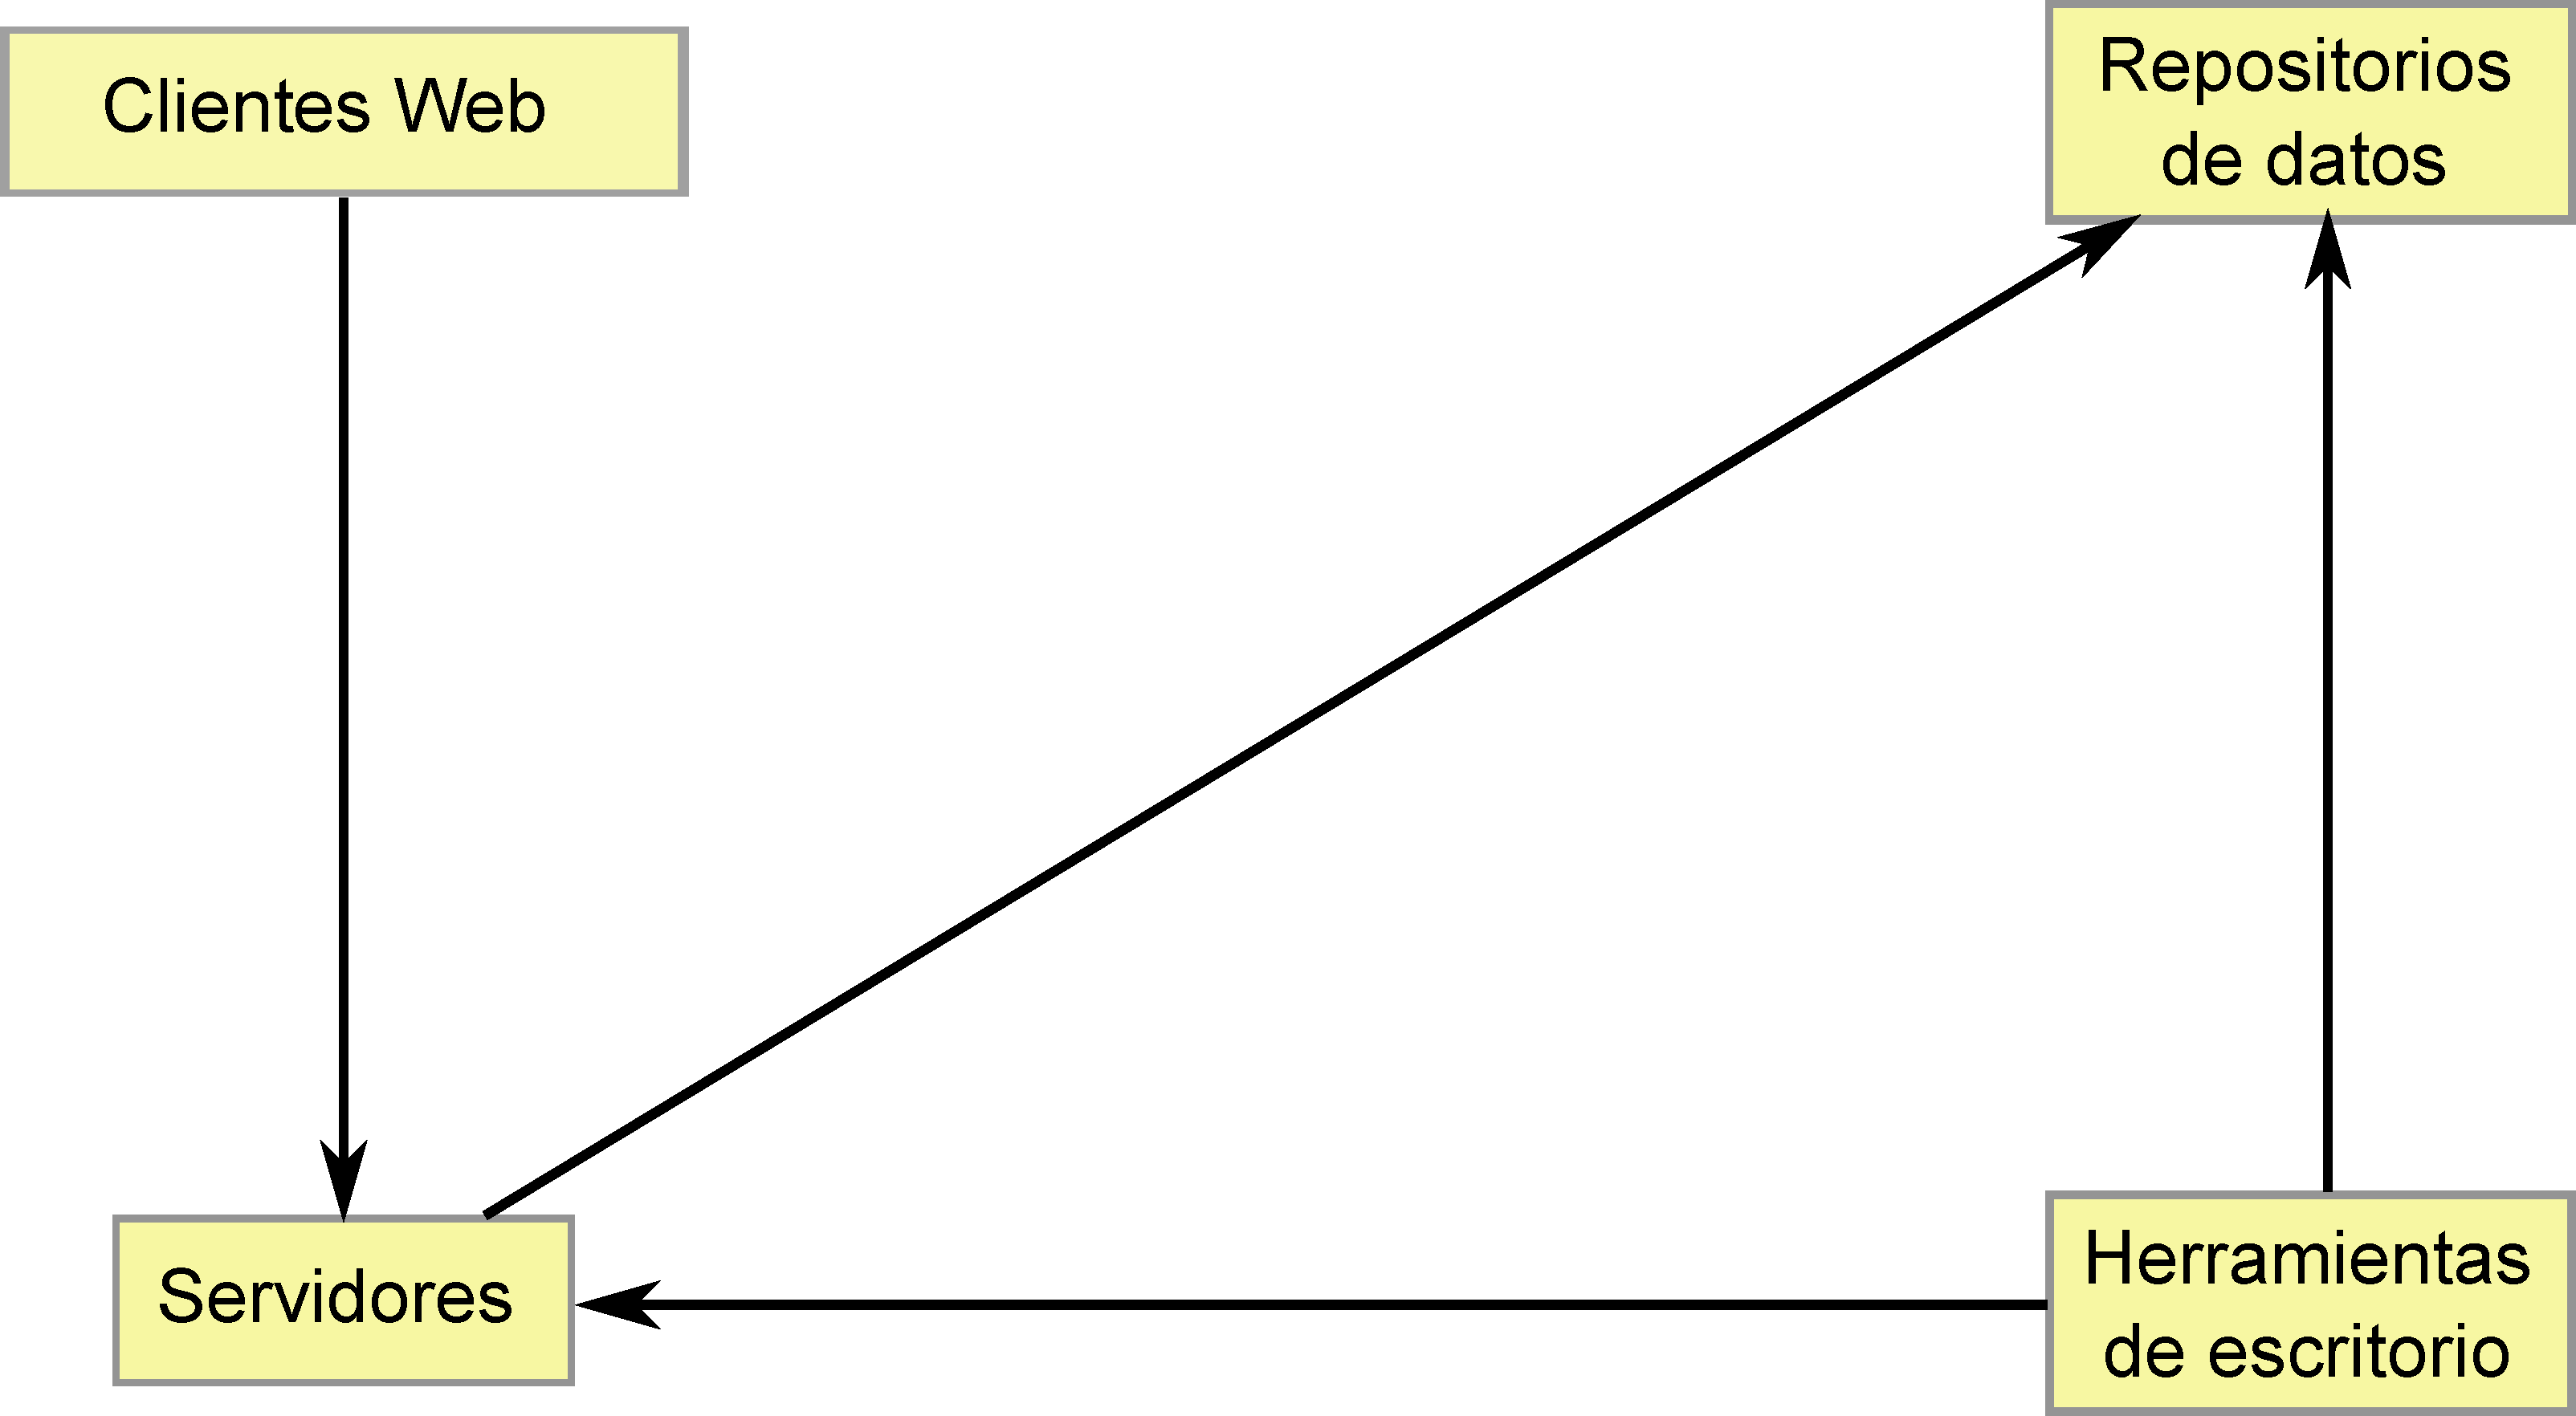
\includegraphics[width=.65\mycolumnwidth]{Introduccion_tecnologia/Esquema_tecnologia_SIG.pdf}
\caption{\small Clases principales de software SIG y relaciones entre ellas}
\label{Fig:Esquema_tecnologia_SIG} 
\end{figure}

\section{La adaptaci�n de las aplicaciones SIG. El SIG como base gen�rica}
	
Los SIG han crecido mucho desde su origen y, adem�s de ampliar horizontes y mejorar el trabajo con ellos, han a�adido numerosas funcionalidades adicionales. Como cabe esperar, un SIG actual no solo permite hacer las cosas mejor, sino que tambi�n permite hacer m�s cosas. Como herramienta rica en capacidades, un SIG puede entenderse como una aplicaci�n preparada para responder a todas las posibles necesidades dentro del campo del an�lisis geogr�fico.

Sin embargo, la filosof�a actual de las aplicaciones SIG es distinta a la existente en los primeros desarrollos, y el objetivo principal de un SIG hoy en d�a no es el de constituir una herramienta que contenga todas las funcionalidades que puedan necesitarse, sino una base sobre la que estas puedan construirse. Junto a las funciones b�sicas de edici�n, manejo de datos y an�lisis, un SIG permite la adaptaci�n de estas a las necesidades concretas de cada trabajo, siendo as� una herramienta vers�til que puede tomar una u otra forma en funci�n de las circunstancias particulares de cada uso.

La adaptabilidad de SIG es una de sus principales virtudes, y es la que permite que puedan desarrollarse �tiles v�lidos para cada caso. Un SIG no es, por tanto, una herramienta cerrada con un conjunto de elementos suficiente para dar respuesta a todas las necesidades, y la obtenci�n de una herramienta SIG final para un determinado trabajo no es un proceso �nico sino un desarrollo en dos etapas. 

La primera de estas etapas implica el desarrollo del propio SIG como tal, y la segunda concierne al desarrollo de elementos adicionales que completan la herramienta seg�n las necesidades propuestas, apoy�ndose sobre los componentes fundamentales. Aunque muchos usuarios tendr�n suficiente con un SIG en su forma original, muchos otros necesitar�n desarrollos adicionales, o bien se beneficiar�n de ellos al poder lograr sustanciales mejoras en comparaci�n con el empleo del SIG b�sico.

Debido a este esquema de trabajo, el usuario SIG ha de ser en ocasiones un usuario t�cnico y cualificado, o bien ha de necesitar el concurso de alguien capaz de desarrollar sobre un SIG herramientas adicionales. La figura del programador SIG es importante dentro de un proyecto SIG, y hace que la gesti�n de la tecnolog�a tenga la misma relevancia que la gesti�n de los datos o de cualquier otro de los restantes componentes globales de un SIG.

La idea de un SIG como herramienta base es especialmente patente en el caso de las aplicaciones de escritorio, las cuales concentran una gran mayor�a del trabajo desarrollado dentro de un proyecto SIG, lo cual las hace especialmente aptas a constituirse como herramientas b�sicas sobre las que se desarrollan modificaciones destinadas a responder a las necesidades del proyecto. No obstante, tambi�n otras aplicaciones SIG son susceptibles de jugar ese mismo papel.

En el caso de las aplicaciones Web, estas se adaptan para crear accesos particulares a unos datos concretos, de forma que pueden emplearse para dar acceso a la informaci�n geogr�fica a trav�s de Internet, y hacerlo de una forma particular en cuanto a la apariencia y las funcionalidades ofrecidas. Los servidores se prestan de igual modo a ser adaptados en la medida de lo necesario.

Aunque la presencia de elementos para facilitar esa adaptabilidad (lenguajes de programaci�n integrados, arquitecturas escalables, etc.) es general, la aparici�n de alternativas libres competitivas dentro del mercado del SIG ha potenciado m�s a�n el desarrollo de herramientas adaptadas, al permitirlo en mayor grado. Puedes encontrar m�s sobre las diferencias entre software libre y software privativo en el apartado \ref{Software_libre_vs_privativo}, con especial atenci�n a las aplicaciones SIG.


\section{Resumen}

A partir de la concepci�n inicial de los SIG como aplicaciones bien definidas en las cuales se reun�an las funcionalidades principales de estos, se ha desarrollado en la actualidad un amplio panorama de aplicaciones bien diferenciadas, las cuales podemos dividir en tres grupos principales: herramientas de escritorio, repositorios de datos y clientes y servidores. 

Estos tipos de aplicaciones se encuentran interrelacionados y se apoyan unos en otros para ofrecer todo el conjunto de capacidades actuales de los SIG.

Para llegar hasta este punto, los SIG han tomado elementos de otras aplicaciones, congreg�ndolos en un �nico software. Al mismo tiempo, se han ido especializando en distintos �mbitos, dividiendo as� el total de �reas de posible trabajo de este tipo de tecnolog�as.

En la actualidad los SIG forman una base gen�rica sobre la cual se construyen herramientas de an�lisis geogr�fico adaptadas a distintos fines.

%\bibliographystyle{unsrt}
%\bibliography{../../Libro_SIG}
\chapter{Herramientas de escritorio}\label{SIGs_escritorio}

\begin{keypoints}
�Qu� entendemos por \emph{herramientas de escritorio}? $\bullet$ �Por qu� se caracterizan y cu�les son las tendencias actuales en su desarrollo? $\bullet$ �Qu� funciones desempe�an dentro del conjunto de herramientas SIG? $\bullet$ �Qu� tipo de tareas podemos desempe�ar con ellas?
\end{keypoints}

\bigskip

\begin{intro}
Las herramientas de escritorio son la forma m�s <<t�pica>> en la que se presentan los Sistemas de Informaci�n Geogr�fica, y que ofrecen elementos para realizar las tareas b�sicas de un proyecto SIG. En este cap�tulo veremos sus caracter�sticas principales y los distintos tipos de ellas que pueden encontrarse, detallando la utilidad de cada una.
\end{intro}

\section{Introducci�n}

El concepto cl�sico de un SIG es el de una aplicaci�n completa en la cual se implementan herramientas para llevar a cabo las tareas b�sicas del trabajo con datos geogr�ficos: creaci�n o edici�n, manejo y an�lisis. Con esta filosof�a fueron desarrollados los primeros programas SIG, especialmente para el tratamiento y an�lisis de datos geogr�ficos y, posteriormente, para dotar a estos de mayor versatilidad, incorporando otras funciones adicionales que facilitaran el trabajo con esos mismos datos. Se tienen as� las herramientas de escritorio, que son aquellas que m�s se asemejan a la concepci�n original de los SIG.

A pesar de que existen, como vimos en el cap�tulo anterior, otras clases de aplicaciones SIG, los SIG de escritorio siguen manteniendo su posici�n como aplicaciones fundamentales, y hablar gen�ricamente de un SIG implica por lo general  hacerlo de una aplicaci�n de escritorio antes que de otros tipos de aplicaciones. Por otra parte, las herramientas de escritorio son soluciones en general completas que cubren la totalidad de necesidades que se presentan en el desarrollo de proyectos SIG, y por ello constituyen las herramientas primordiales para llevar estos a cabo.

\section{Funciones b�sicas}

Podemos dividir las funciones b�sicas de un SIG de escritorio en cinco bloques: entrada y salida de datos, visualizaci�n, edici�n, an�lisis y generaci�n de cartograf�a. Una aplicaci�n de escritorio habitual presenta todas estas capacidades en cierta medida, aunque no necesariamente con el mismo nivel de implementaci�n.

\subsection{Entrada y salida de datos}

Ya sabemos que los datos son una parte imprescindible de un SIG, y sin ellos no puede desarrollarse actividad con una aplicaci�n SIG. Por esta raz�n, todas estas aplicaciones deben obligatoriamente implementar capacidades para leer datos y, opcionalmente, para guardarlos. Esta ultima es necesaria en el caso en que el SIG pueda generar nuevos datos geogr�ficos (nuevas capas), pero no en aquellas aplicaciones sin capacidades de an�lisis o edici�n, donde su empleo no ha de crear nuevos datos.

Pese a ser de tal importancia, la implementaci�n de las capacidades de entrada y salida es muy variable en unos u otros SIG. Una raz�n por la que esto sucede es el gran n�mero de formatos de fichero distintos, la cual no favorece la interoperabilidad, como ya vimos en el cap�tulo \ref{Fuentes_datos}. As�, cada SIG es capaz de abrir unos u otros formatos de archivo, y mientras que algunos tratan a todos ellos por igual, ciertas aplicaciones\footnote{Como, por ejemplo, ILWIS o SAGA, que veremos en el anexo \ref{Panorama_actual}} trabajan en un formato propio con car�cter nativo, y son capaces de incorporar datos en otros formatos a trav�s de extensiones o funciones de conversi�n entre estos y el formato particular del programa.\index{ILWIS}\index{SAGA}

La existencia de librer�as y componentes de acceso a datos en los que las aplicaciones SIG de escritorio pueden apoyarse mejora la conectividad entre estas y aporta cierta homogeneidad en este aspecto.

Otra diferencia importante en la gesti�n de los datos es la capacidad de conexi�n a bases de datos o servicios remotos como los que veremos en el cap�tulo \ref{Servidores_y_clientes_remotos}\footnote{B�sicamente, estos servicios van a permitir acceder a datos geogr�ficos que no est�n en nuestro ordenador, del mismo modo que accedemos a textos o im�genes a trav�s de un navegador Web}. As�, algunas aplicaciones tienen �nicamente capacidades de abrir archivos, pero no de acceder a servicios remotos, mientras que otras pueden acceder a todo tipo de or�genes de datos. Las aplicaciones que acceden a servicios remotos entran dentro de la denominaci�n de \emph{clientes}. Los clientes Web que veremos en el cap�tulo \ref{Servidores_y_clientes_remotos} se conocen como clientes \emph{ligeros}, mientras que las aplicaciones SIG de escritorio con estas capacidades se denominan clientes \emph{pesados}, haciendo referencia a su mayor volumen y el mayor n�mero de funcionalidades que contienen. La funcionalidad que ofrecen en relaci�n al acceso a datos remotos es similar en ambos casos, y la trataremos en el citado cap�tulo \ref{Servidores_y_clientes_remotos} con detalle.\index{Cliente!ligero}\index{Cliente!pesado}

En general, las capacidades de acceso a servicios remotos est�n en funci�n del enfoque de la aplicaci�n, y aquellas fuertemente enfocadas al an�lisis no suelen presentar tales funcionalidades, mientras que aquellas m�s orientadas a la visualizaci�n o las herramientas globales m�s completas s� que las incorporan.

\subsection{Visualizaci�n}\label{Funcion_SIG_Visualizacion}

La visualizaci�n es una funci�n fundamental dentro de los SIG y del trabajo con cartograf�a en general. En este libro, por ejemplo, existe una parte completa dedicada a esta materia, pues su conocimiento resulta fundamental para poder aprovechar plenamente la informaci�n contenida en el dato geogr�fico.

Aunque existen SIG que no incorporan capacidades de visualizaci�n o estas no son muy avanzadas, la gran mayor�a de las herramientas de escritorio incluyen un gran n�mero de elementos para representar los datos geogr�ficos con los que se trabaja. En ocasiones, interesa �nicamente crear una representaci�n de los datos, pero incluso cuando el trabajo con una herramienta SIG est� enfocado a la realizaci�n de un an�lisis, la visualizaci�n y exploraci�n visual de los datos de partida es un paso previo.

En general, la forma de operar con los elementos de visualizaci�n es muy similar entre soluciones SIG distintas y, a diferencia de lo que sucede con la implementaci�n de otras funcionalidades, el manejo es pr�cticamente igual. Esto sucede no solo ya en las herramientas de escritorio que tratamos en este cap�tulo, sino tambi�n en las que veremos en el dedicado a las aplicaciones Web, las cuales incorporan tambi�n capacidades de visualizaci�n del mismo tipo. En ambos casos, las herramientas fundamentales presentan una estructura similar y unos conceptos base muy parecidos.

Esta estructura se compone fundamentalmente de un lienzo sobre el que se sit�an las distintas capas de informaci�n geogr�fica, y que el usuario va conformando a�adiendo nuevas capas y editando la forma en la que estas se representan. Las capas se sit�an en un orden dado dentro del lienzo, lo que permite establecer una jerarqu�a de representaci�n y as� lograr el aspecto deseado.

Junto a este lienzo existen herramientas de navegaci�n que permiten ampliar o reducir la escala, o bien modificar el encuadre (Figura \ref{Fig:Herramientas_navegacion}). Asimismo, se presentan todas las funciones que permiten obtener las distintas formas de representaci�n que veremos en la parte \ref{Visualizacion}, tales como el ajuste de colores o el establecimiento de etiquetas en funci�n de los valores asociados a las distintas entidades, entre otros.

\begin{figure}[!hbt]
\centering
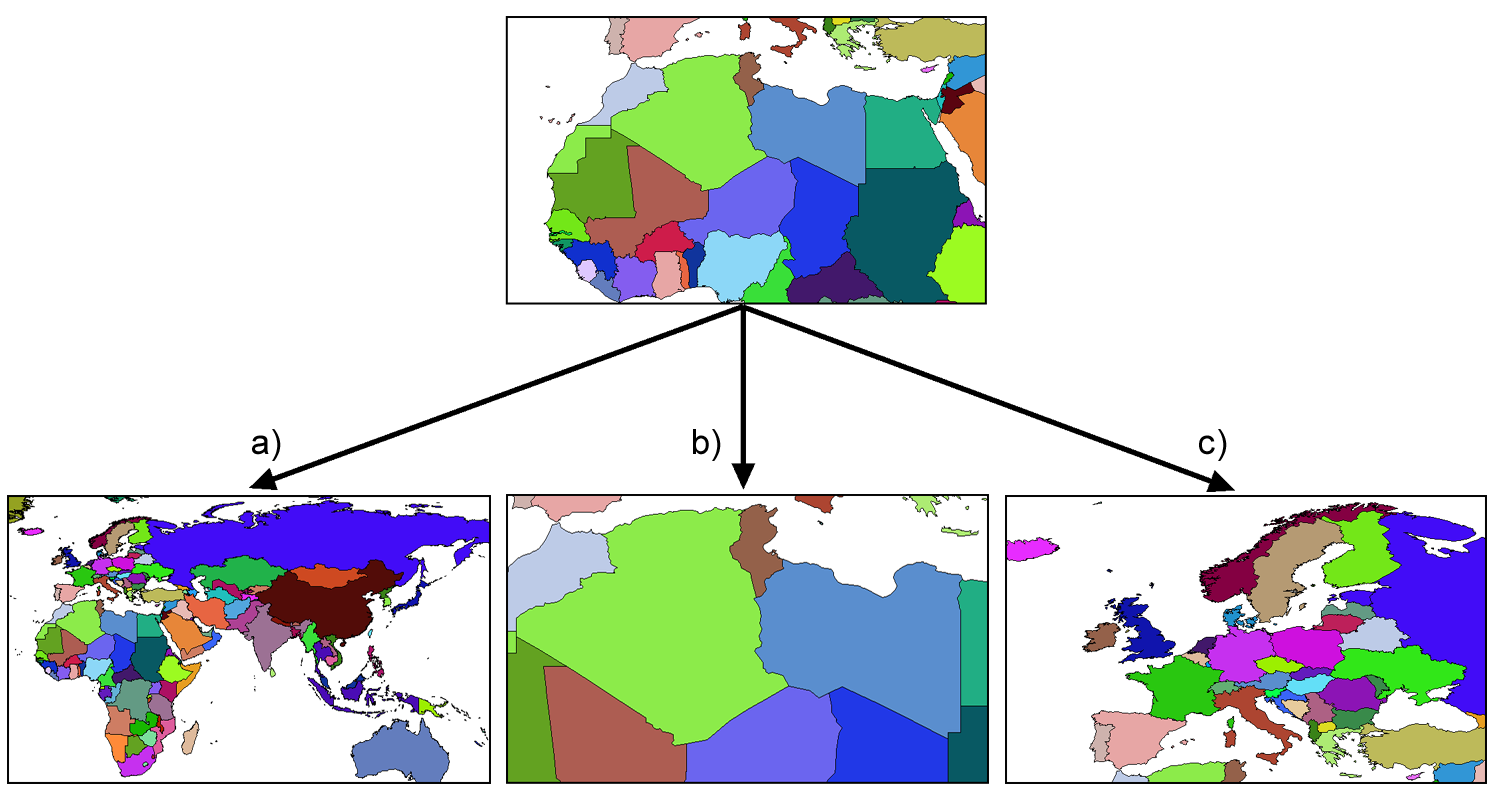
\includegraphics[width=.75\textwidth]{SIGs_escritorio/Herramientas_navegacion.png}
\caption{\small Herramientas de navegaci�n fundamentales en el entorno gr�fico de un SIG de escritorio. a) alejamiento (\emph{zoom out}), b) acercamiento (\emph{zoom in}), c) desplazamiento (\emph{pan})}
\label{Fig:Herramientas_navegacion} 
\end{figure}

Estas capacidades convierte a los datos geogr�ficos en un elemento activo, pues, a diferencia de un mapa cl�sico donde no pueden modificarse sus caracter�sticas, en un SIG el usuario puede de forma r�pida y sencilla elegir \emph{qu�} ve y \emph{c�mo} lo ve.

Como parece l�gico pensar, la visualizaci�n ha evolucionado mucho desde los primeros SIG, y ha ido progresivamente adquiriendo nuevas capacidades, muchas de las cuales solo son posibles con los modernos componentes gr�ficos de los ordenadores actuales. As�, adem�s de ofrecer mayores posibilidades de personalizaci�n, el uso del SIG como herramienta de representaci�n permite obtener resultados novedosos que a�aden nuevas formas de explorar los datos geogr�ficos y trabajar con ellos.

En el caso m�s habitual, la representaci�n de una capa en un lienzo de un SIG es bidimensional, de la misma forma que se representa en un mapa impreso, lo cual se debe tanto a la mayor facilidad de implementaci�n de este tipo de representaciones como a la mayor exigencia que otro tipo de representaciones presentan en lo referente al equipo (\extr{hardware}). 

No obstante, la presencia de visores tridimensionales est� experimentando un gran crecimiento en los �ltimos a�os, y se van integrando paulatinamente dentro de los SIG para ofrecer una nueva forma de representaci�n. Esta clase de capacidades gr�ficas, inalcanzables en t�rminos de rendimiento para un equipo com�n hace unos a�os, son hoy d�a perfectamente utilizables en un ordenador de consumo habitual, y aportan una nueva forma de trabajar con los datos geogr�ficos.

Las funcionalidades de representaci�n 3D a�n no se integran completamente dentro del entorno de un SIG de escritorio completo, ya que se conciben por lo general como un elemento puramente visual y enfocado a la representaci�n como tal, mientras que un lienzo 2D cumple su funci�n tradicional de marco de trabajo sobre el que se desarrollan las restantes tareas del SIG como el an�lisis o la propia gesti�n de datos. Aun as�, conforme las vistas tridimensionales se van convirtiendo en elementos habituales, los restantes componentes del SIG se van coordinando con ellas para darles a su vez la capacidad de servir como entornos de trabajo vers�tiles.

La presencia de una dimensi�n adicional hace que las herramientas de navegaci�n sean m�s complejas en el caso tridimensional, existiendo ajustes relativos a la perspectiva, a los �ngulos de visi�n o a la exageraci�n del relieve, entre otros par�metros. Como puede verse m�s adelante en la figura \ref{Fig:GEarth}, las herramientas de control de navegaci�n de un visor 3D (situadas en este caso en la parte superior derecha de la figura) , son sensiblemente m�s complejas que las herramientas base del caso 2D, presentadas en la figura \ref{Fig:Herramientas_navegacion}.

Esta mayor complejidad hace asimismo que puedan existir diversas formas en las que las capacidades de visualizaci�n 3D se presentan en un SIG. Las representaciones tridimensionales pueden ser simples representaciones en relieve de una capa (Figura \ref{Fig:Tipos_vistas_3D}a), o pueden incluir verdaderos elementos en tres dimensiones (Figura \ref{Fig:Tipos_vistas_3D}b). En el primer caso, la capa no contiene datos de elevaci�n (puede ser por ejemplo una capa de usos de suelo), y la representaci�n tridimensional se realiza bas�ndose en la informaci�n de una capa adicional de elevaciones (que denomin�bamos de 2,5D por no poder representar todo tipo de formas en el espacio). La capa plana se representa en espacio <<deformada>> para ajustarse al relieve existente en la zona que representa.\index{Vista 3D}

En el caso de una representaci�n tridimensional real, los objetos poseen informaci�n sobre su forma tridimensional, y junto con las coordenadas que delimitan su geometr�a plana (las geometr�as b�sicas que conocemos: punto, l�nea y pol�gono), existen valores adicionales en el eje vertical. De este modo, pueden representarse entidades tales como edificios, o una ruta tridimensional que represente la trayectoria de un avi�n. Asimismo, y como puede verse en la figura, pueden a�adirse elementos adicionales que aprovechan las capacidades de representaci�n 3D, as� como etiquetas o incluso elementos interactivos que tambi�n act�an en 3D (por ejemplo, para la selecci�n de entidades).


\begin{figure}[!hbt]
\centering
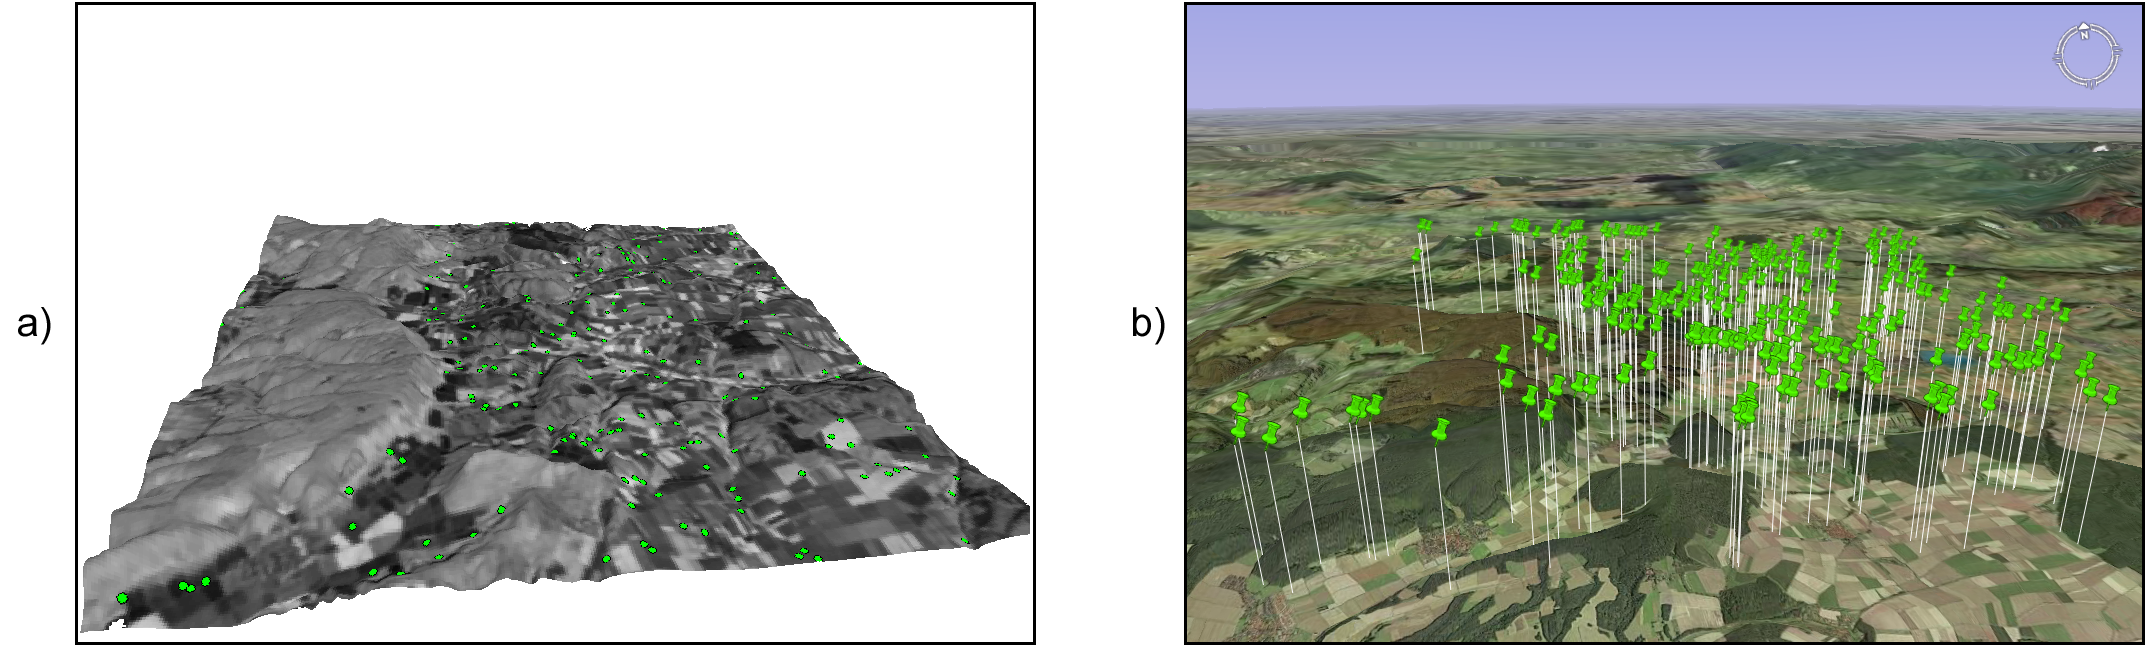
\includegraphics[width=.9\textwidth]{SIGs_escritorio/Tipos_vistas_3D.png}
\caption{\small Distintas formas de representaci�n 3D de capas de datos geogr�ficos}
\label{Fig:Tipos_vistas_3D} 
\end{figure}

Es importante recalcar que la visualizaci�n de una capa dentro de un SIG es independiente de la informaci�n que dicha capa contiene o la forma en que esta se almacena. El dato geogr�fico y su representaci�n van por separado, y el dato en s� no define la representaci�n, sino que �nicamente sirve como apoyo para esta. Esto es particularmente cierto para el caso de capas vectoriales, as� como para capas r�ster que contengan un valor de tipo no gr�fico, es decir, aquellas que no sean im�genes.

Una imagen tendr� el mismo aspecto en todos los SIG en los que se utilice, puesto que la informaci�n relativa a su representaci�n se contiene, al menos en cierta medida, en la propia imagen. Los valores de la imagen representan una intensidad de luz y, si las bandas corresponden a la zona del visible, existe asimismo una informaci�n de colores. Otras im�genes pueden proceder del escaneo de un mapa o una fotograf�a impresa, y en ese caso recogen tambi�n los colores de cada p�xel. \index{Escaneo}

Aun en el caso de im�genes con m�s de tres bandas, en las que no existe una correspondencia directa entre los valores y la representaci�n (tal como vimos, por ejemplo, en la creaci�n de representaciones en falso color en el apartado \ref{Visualizacion_imagenes}), puede existir una representaci�n \emph{por defecto} tomando, por ejemplo, las tres primeras bandas, y sigue siendo probable que estas im�genes tambi�n se vean de igual modo en uno u otro SIG (aunque luego ello no implica que dicha representaci�n no pueda ajustarse a conveniencia en todos los casos).\index{Falso color}

En el caso de capas vectoriales o una capa r�ster tal como un MDE, no existe ning�n tipo de informaci�n acerca de la representaci�n acompa�ando al dato espacial en s�. Los datos necesitan de un esquema de asignaci�n que los convierta en elementos visuales (colores, texturas, etc.), pero este esquema es ajeno al dato en s�. 

La labor del SIG relativa a la visualizaci�n consiste en <<interpretar>> los datos y convertirlos en representaciones, y para ello se basa en esquemas definidos por el usuario. Estos esquemas pueden ser almacenados de forma que en sucesivos usos de una capa de datos, esta se represente de una misma forma. No obstante, abrir la capa con una aplicaci�n SIG distinta implicar� en general perder las caracter�sticas definidas para su representaci�n ya que, si bien los formatos de datos son relativamente interoperables, no as� los formatos en que se almacenan los criterios de representaci�n de esos datos.

Est�ndares para el almacenamiento de estilos como SLD(\extr{Styled Layer Descriptor}), que veremos en detalle en el apartado \ref{SLD}, tienen como objeto solventar este problema. \index{SLD}

\subsection{An�lisis}

Si hubi�ramos de ordenar cronol�gicamente las distintas funcionalidades que un SIG de escritorio presenta, probablemente el an�lisis fuera una de las primeras. Por encima de otras capacidades, los ordenadores han sido y son principalmente herramientas de c�lculo capaces de realizar operaciones y computar resultados, y este ha sido uno de los usos fundamentales relativos al manejo de datos geogr�ficos. Otros usos, tales como la visualizaci�n, pese a ser pr�cticamente imprescindibles hoy en d�a, estaban muy limitados en los primeros SIG. No ocurr�a as� en el �mbito del an�lisis ya que, aunque con capacidades como es l�gico menores que las actuales, los ordenadores ofrec�an una potencia de calculo que los convert�a en herramientas de an�lisis tan interesantes como en la actualidad.

La tendencia actual en los SIG es considerar las capacidades de an�lisis como herramientas modulares que se ejecutan sobre una plataforma base, la cual comprende las capacidades de visualizaci�n y entrada y salida de datos. Todas estas capacidades de an�lisis son independientes entre s�, aunque pueden coordinarse y emplearse en conjunto para alcanzar un resultado concreto. De otro modo, cada una de las formulaciones o algoritmos que vimos en los cap�tulos de la parte \ref{Procesos} aparece dentro del SIG como una herramienta individual que opera sobre una serie de capas y genera un resultado dado, tomando en muchas ocasiones esas capas de entre aquellas que se est�n representando en el SIG, e incorporando asimismo a dicha representaci�n las nuevas capas generadas.

Las herramientas de an�lisis pueden aparecer igualmente como programas independientes, y el SIG de escritorio ser una herramienta aglutinadora que centraliza estas, facilitando su uso y la gesti�n de los datos implicados en los procesos de an�lisis.

Cuando las herramientas de an�lisis utilizan directamente la base del SIG donde se encuentran las capacidades de visualizaci�n y manejo de datos, puede existir cierto grado de interactividad. Las operaciones de consulta, por ejemplo, las cuales vimos en el cap�tulo \ref{Consultas}, son en general de este tipo, ya que el usuario puede actuar sobre el lienzo para hacer una selecci�n de modo gr�fico. M�s a�n, esa selecci�n puede condicionar los posteriores an�lisis sobre la capa cuyas entidades se seleccionan, ya que los procesos que operen sobre ella pueden restringir su alcance a aquellas entidades seleccionadas.\index{Consultas}

En caso de no existir este tipo de interacci�n entre elementos de an�lisis y elementos de visualizaci�n y exploraci�n de datos, los procesos de an�lisis suelen constituir utilidades autocontenidas que simplemente toman una serie de datos de entrada, realizan un proceso en el que el usuario no interviene, y finalmente generan un resultado con car�cter definitivo. Este resultado podr� ser posteriormente visualizado o utilizado como entrada para un nuevo an�lisis.

A modo de ejemplo, podemos analizar el caso particular del c�lculo de una ruta que conecte una serie de puntos a trav�s de una red (los fundamentos de este an�lisis los vimos en el apartado\ref{Analisis_redes}). \index{Ruta �ptima}

Una de las formas de implementar este an�lisis es aquella que requiere del usuario la introducci�n de la informaci�n necesaria (una capa de lineas con la red viaria y otra de puntos con los puntos de inicio, paso, y llegada correspondientemente ordenados) como par�metros que el proceso toma y en funci�n a los cuales se genera una nueva capa. El proceso es una tarea perfectamente definida, con unas entradas y una salidas, y tras la selecci�n de unas capas de entrada se genera un nuevo resultado en forma de otra capa. Este proceso puede implementarse de forma aislada del SIG, aunque coordinada con �l para lograr mejores resultados y una utilizaci�n m�s sencilla.\index{Interactividad}

Otra forma con un enfoque distinto ser�a presentando un proceso interactivo en el cual se introduce como �nico par�metro inicial la red viaria. Posteriormente, el usuario puede operar sobre el lienzo en el que esta se encuentra representada para ir definiendo y editando la lista de puntos de paso. El c�lculo se va efectuando cuando se produce alg�n cambio en la misma y debe aplicarse de nuevo el algoritmo pertinente para adaptar el resultado ---la ruta �ptima--- a ese cambio.

Este tipo de formulaciones interactivas son m�s intuitivas y agradables de usar, pero en realidad menos productivas de cara a un trabajo dentro de un proyecto SIG. Aparecen por ello en aquellas funciones que tienen una mayor componente visual o, especialmente, en las que representan un an�lisis puntual que se realiza de forma com�n como algo individual. Estos son los an�lisis que se implementan en las aplicaciones que veremos m�s adelante como parte del grupo de SIG enfocados a la exploraci�n visual de datos geogr�ficos, que adem�s de esta proveen alguna serie de utilidades de an�lisis, pocas en general, sin que estas est�n concebidas para un trabajo completo en un proyecto SIG de cualquier �ndole, sino m�s bien para un uso ocasional.

En un proyecto SIG de cierto tama�o, lo m�s com�n es que la fase de an�lisis, a la que seguir� una fase tambi�n compleja de preparaci�n e interpretaci�n de resultados, y previa a la cual se ha debido llevar a cabo la preparaci�n de los datos de partida, comprenda no uno sino muchos an�lisis distintos. Estos an�lisis, a su vez, no son independientes, sino que est�n relacionados entre s� y lo m�s habitual es que definan como tales un flujo de trabajo que comienza en los datos de partida y desemboca en los resultados finales a trav�s de una serie de procesos. 

Por su naturaleza, tanto los datos espaciales como los procesos en los que estos intervienen se prestan a formar parte de estos flujos de trabajo m�s o menos complejos, y es por ello que en los SIG actuales una funcionalidad b�sica es la creaci�n de tareas complejas que permiten simplificar todo un proceso de muchas etapas en una �nica que las engloba a todas. La forma anteriormente comentada en que aparecen las formulaciones dentro de un SIG, de forma atomizada y modular, facilita la creaci�n de estos <<modelos>> a partir de procesos simples.

Para entender esta idea, podemos ver un ejemplo aplicado. La extracci�n de una red de drenaje en formato vectorial a partir de un MDE requiere una serie de procesos, a saber (para repasar los fundamentos de cada uno de estos procesos y comprender mejor la operaci�n global, puede consultarse el cap�tulo \ref{Geomorfometria}, donde se describieron en su momento, as� como la secci�n \ref{Vectorizacion_lineas}):

\begin{enumerate}
	\item Eliminaci�n de depresiones del MDE.
	\item C�lculo de una capa de �rea acumulada a partir del MDE corregido
	\item Extracci�n de capa r�ster con la red de drenaje a partir de la capa anterior y un valor umbral
	\item Vectorizaci�n de la capa resultante del paso anterior
\end{enumerate}

\index{Modelo Digital de Elevaciones}

Lo anterior podr�a simplificarse si se agruparan en una sola operaci�n todos los procesos anteriores, de forma que tomando dos datos de entrada (un MDE y un umbral), se realizara todo el proceso de forma continua. Las capacidades de creaci�n de modelos que implementan los SIG de escritorio (en particular, los m�s enfocados al an�lisis) permiten crear nuevos procesos compuestos utilizando entornos gr�ficos intuitivos, y estos procesos pasan a formar parte del conjunto de ellos de que dispone el SIG, permitiendo que cada usuario <<resuma>> en procesos unitarios una serie de operaciones que, de otro modo, deber�an realizarse de forma individual con el coste operacional que ello implica.

Una vez que se ha creado un proceso compuesto, este puede aplicarse sobre nuevos datos de entrada, reduci�ndose as� el tiempo y la complejidad con que nuevos par�metros de entrada pueden ser procesados seg�n el esquema de trabajo definido en dicho proceso.

Debe pensarse que el proceso presentado como ejemplo es muy sencillo y �nicamente implica cuatro operaciones encadenadas de forma lineal. Un proceso de an�lisis habitual puede contener muchas m�s operaciones individuales, y estas disponerse de forma m�s compleja, con dependencia de distinta �ndole entre sus resultados. La imagen \ref{Fig:Proceso_complejo} muestra el aspecto de uno de tales procesos implementado en un software (ArcGIS, v�ase secci�n \ref{Soft_privativo}) con capacidad de de creaci�n de modelos. El proceso representado en la figura \ref{Fig:Esquema_MonteCarlo} tambi�n es un ejemplo de otro tipo de an�lisis que puede adaptarse ventajosamente en este tipo de herramientas de modelizaci�n.\index{ArcGIS}

\begin{figure}[!hbt]
\centering
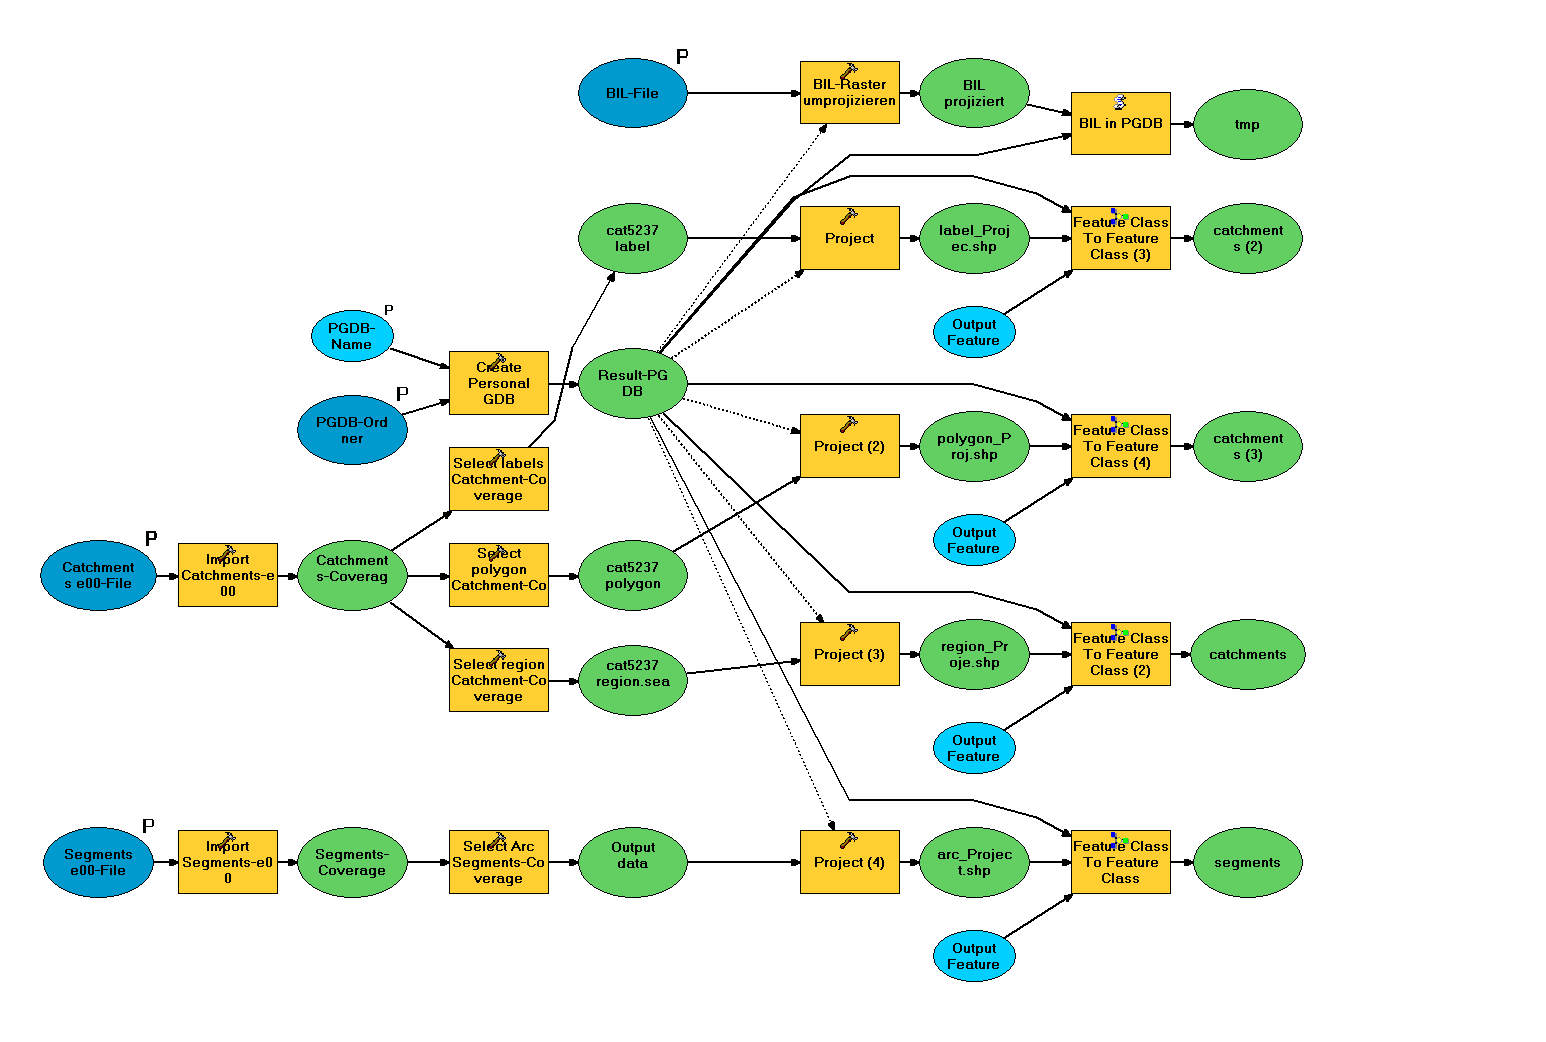
\includegraphics[width=.9\textwidth]{SIGs_escritorio/Proceso_complejo.png}
\caption{\small Esquema de un proceso complejo creado a partir de operaciones simples de an�lisis con datos SIG.}
\label{Fig:Proceso_complejo} 
\end{figure}

\subsection{Edici�n}

Los datos geogr�ficos con los que trabajamos en un SIG no son una realidad est�tica. La informaci�n contenida en una capa es susceptible de ser modificada o corregida, y las funciones que permiten estas tareas son importantes para dotar al SIG de versatilidad. Sin ellas, los datos espaciales pierden gran parte de su utilidad dentro de un SIG, ya que se limitan las posibilidades de trabajo sobre estos. Las funcionalidades de edici�n son, por tanto, b�sicas en una herramienta de escritorio.

Las operaciones de edici�n pueden emplearse, por ejemplo, para la actualizaci�n de cartograf�a. Como vimos en el cap�tulo \ref{Fuentes_datos}, una de las ventajas de los datos digitales frente a los anal�gicos es la mayor facilidad de actualizaci�n. As�, si una entidad en una capa vectorial (por ejemplo, una parcela catastral) modifica su geometr�a, no es necesario rehacer todo un mapa, sino simplemente editar ese elemento. A lo largo del desarrollo de un proyecto SIG, es muy probable que sea necesario editar de un modo u otro alg�n dato espacial, bien sea para corregirlo, ampliarlo, mejorarlo o sencillamente adaptarlo a las necesidades del propio proyecto.

Adem�s de la modificaci�n de una capa ya existente, las herramientas de edici�n de un SIG de escritorio se emplean igualmente para la creaci�n de capas nuevas, que pueden crearse a partir de la digitalizaci�n de im�genes como vimos en el cap�tulo \ref{Fuentes_datos}, o bien en base a cualquier otra capa de la que dispongamos.

Aunque las tareas de edici�n m�s habituales son las relacionadas con la edici�n de geometr�as, no es esta la �nica edici�n que puede realizarse dentro de un SIG. Podemos distinguir las siguientes formas de edici�n:

\begin{itemize}
\item Edici�n de geometr�as de una capa vectorial
\item Edici�n de atributos de una capa vectorial
\item Edici�n de valores de una capa r�ster
\end{itemize}

Las herramientas destinadas a la edici�n de entidades geom�tricas heredan sus caracter�sticas de los programas de dise�o asistido por ordenador (CAD), cuya funcionalidad principal es precisamente la edici�n de elementos gr�ficos. Estas incluyen la adici�n o eliminaci�n de nuevas geometr�as, la modificaci�n de ellas editando sus puntos (recordemos que toda entidad vectorial se reduce a un conjunto de puntos en �ltima instancia), as� como otras operaciones geom�tricas b�sicas. En la secci�n \ref{Digitalizacion_manual} vimos algunas de ellas a la hora de tratar la calidad de la digitalizaci�n en pantalla.\index{CAD}

Otras funciones de edici�n que encontramos son las que permiten simplificar algunas tareas, tales como la divisi�n de un pol�gono. La figura  \ref{Fig:Division_poligono} muestra c�mo un pol�gono puede dividirse en dos simplemente trazando una l�nea divisoria.  Otras funcionalidades similares incluyen la eliminaci�n autom�tica de pol�gonos esp�reos (v�ase \ref{Poligonos_espureos}), o el ajuste autom�tico entre entidades.\index{Pol�gono!espureo}

\begin{figure}
\centering

\includegraphics[width=.65\mycolumnwidth]{SIGs_escritorio/Division_poligono.pdf}
\caption{\small Divisi�n autom�tica de un pol�gono en dos nuevas entidades a partir de una l�nea. Funcionalidades de este tipo aparecen en los SIG para facilitar las tareas de edici�n.}
\label{Fig:Division_poligono} 
\end{figure}

En general, el n�mero de funcionalidades es sensiblemente menor que en el caso de los programas CAD, ya que gran parte de ellas no tiene aplicaci�n directa en el caso de trabajar con datos geogr�ficos. No obstante, tambi�n aparecen herramientas adicionales, como sucede en el caso de que se registre informaci�n topol�gica, lo cual ha de considerarse por igual en el proceso de edici�n. As�, herramientas como la mostrada en la figura \ref{Fig:Division_poligono} han de tener en cuenta la existencia de una estructura topol�gica y un modelo de representaci�n particular en el SIG, y no operar�n igual en todas las aplicaciones, ya que, como sabemos, no todas presentan las mismas capacidades en este terreno.

Junto con las propias geometr�as que pueden editarse seg�n lo anterior, toda capa vectorial tiene asociado un conjunto de atributos, y estos deben poder editarse tambi�n desde el SIG. De hecho, la adici�n de una nueva geometr�a a una capa vectorial no est� completa hasta que no se a�aden igualmente sus atributos.

La edici�n de toda la informaci�n alfanum�rica relacionada con las distintas entidades se realiza en un SIG a trav�s de elementos tomados del �mbito de las bases de datos, siendo esto en general v�lido tanto en lo referente a las interfaces como en el propio acceso a datos. Las operaciones de edici�n de atributos abarcan tanto la modificaci�n de valores sencillos como la de la propia estructura del conjunto de atributos (adici�n o eliminaci�n de columnas ---campos--- en la tabla correspondiente). Por supuesto, la edici�n de atributos y de geometr�as esta �ntimamente relacionada.

Por �ltimo, la edici�n de capas r�ster es mucho menos frecuente, y una gran mayor�a de SIG no permiten la modificaci�n directa de los valores de las celdas. Las operaciones del �lgebra de mapas permiten modificar los valores de una capa y obtener nuevas capas con esos valores modificados, pero editar directamente un valor de celda del mismo modo que se editan el valor de un atributo o la posici�n de un punto de una capa vectorial no es una funcionalidad tan habitual.

Este tipo de capacidades, no obstante, pueden ser de gran utilidad, especialmente en SIG orientados al manejo principal de capas r�ster, donde sustituyen en cierta medida a las funcionalidades de edici�n vectorial equivalentes.

\subsection{Generaci�n de cartograf�a}\label{GeneracionCartografia}

A pesar de que la representaci�n de las distintas capas de datos espaciales en un lienzo es suficientemente potente a efectos de explorar visualmente la informaci�n que estas contienen, la mayor�a de los SIG incorporan capacidades de creaci�n de cartograf�a impresa, generando un documento cartogr�fico que posteriormente puede imprimirse y emplearse como un mapa cl�sico. Las razones para la existencia de tales funcionalidades son muchas, pero la principal sigue siendo la necesidad general que a�n existe de apoyarse en esa clase de documentos cartogr�ficos para poder incorporarlos a proyectos o estudios como parte de anexos cartogr�ficos.

Aunque la representaci�n dentro de un SIG ofrece posibilidades mayores (cambio de escala, ajuste de los par�metros de visualizaci�n, etc.), disponer de una copia <<est�tica>> de cada bloque de informaci�n con el que se trabaja en un SIG es una necesidad ineludible. M�s que una capacidad necesaria para la presentaci�n adecuada de la informaci�n cartogr�fica, la generaci�n de cartograf�a impresa es en muchos casos la principal raz�n para el uso de un SIG. Mientras que las capacidades de an�lisis o edici�n son en ocasiones poco o nada utilizadas, las de generaci�n de cartograf�a son un elemento fundamental, y muchos usuarios la consideran err�neamente como la funcionalidad primordial de un SIG.

Llegado a este punto del libro, y tras todo lo que hemos visto, queda claro, no obstante, que un SIG es ante todo una herramienta de gesti�n y an�lisis de datos espaciales, y que las capacidades enfocadas a la producci�n cartogr�fica deben verse como una ayuda ---de vital importancia, eso s�--- para la presentaci�n final de todo el trabajo que se lleva a cabo en �l.

Fundamentalmente, estas capacidades permiten la composici�n de documentos cartogr�ficos de acuerdo con un dise�o dado, y la impresi�n directa de estas en alg�n perif�rico tal como una impresora com�n o un \emph{plotter} de gran formato. En la elaboraci�n de dicho dise�o, pueden emplearse todos los elementos que habitualmente podemos encontrar en un mapa: el propio mapa en s� (la representaci�n de la informaci�n geogr�fica), leyenda, t�tulo, escala, etc. Con estos elementos, se crea una versi�n autocontenida de la informaci�n geogr�fica, que puede ya emplearse de modo independiente del SIG.\index{Plotter}

Las funciones de dise�o que se implementan por regla general en un SIG son similares a las que pueden encontrarse en un software de maquetaci�n gen�rico, permitiendo la composici�n gr�fica del documento general y el ajuste de los distintos elementos que lo forman. Funciones m�s avanzadas no est�n presentes de modo habitual, principalmente debido a las caracter�sticas muy concretas y bien definidas del tipo de documento con el que se trabaja, lo cual hace posible esta simplificaci�n.

Aunque, como se ha dicho, muchos usuarios, bien por desconocimiento o falta de formaci�n en la herramienta, consideran que la capacidad principal de un SIG es <<hacer mapas>>, lo cierto es que, incluso en aquellas aplicaciones m�s completas y avanzadas, la potencia en la producci�n cartogr�fica es muchas veces insuficiente para producir cartograf�a profesional. Pueden obtenerse resultados de gran calidad y sin duda de suma utilidad, pero lo m�s habitual es no encontrar en un SIG las capacidades que se necesitan, no ya �nicamente desde el punto de vista del cart�grafo, sino desde la perspectiva del dise�o. 

La creaci�n de un mapa no es solo una tarea t�cnica, sino asimismo una labor art�stica, existiendo unas necesidades en funci�n del enfoque que prime. Como herramienta de trabajo, un SIG es un elemento t�cnico, y las consideraciones art�sticas, aunque pueden en cierta forma aplicarse con las herramientas que este implementa, resultan m�s sencillas de tratar si se dispone de aplicaciones m�s espec�ficas en ese sentido.  

Por ello, lograr un mapa de apariencia realmente profesional requiere unas herramientas de dise�o avanzado, a la par que un conjunto de utilidades suficiente como para poder aplicar a la creaci�n del mapa todos los conceptos sobre representaci�n que veremos en la parte \ref{Visualizacion}, no encontr�ndose estas en ocasiones en su totalidad dentro de un SIG. La utilizaci�n del SIG como aplicaci�n base y el uso posterior de programas de dise�o es la soluci�n adecuada para la obtenci�n de cartograf�a profesional, aunque l�gicamente requiere unos mayores conocimientos y una especializaci�n m�s all� de la propia pr�ctica cartogr�fica.

No obstante, para el usuario t�cnico de SIG (el usuario al que est� dirigido este libro), las herramientas de dise�o cartogr�fico que la mayor�a de aplicaciones implementan son m�s que suficientes, y permiten lograr resultados altamente satisfactorios.

Una de las funciones m�s interesantes de generaci�n cartogr�fica en un SIG es la automatizaci�n del proceso y la simplificaci�n de la producci�n de grandes vol�menes de cartograf�a. Por una parte, todas las herramientas de escritorio capaces de producir cartograf�a son a su vez capaces de <<reutilizar>> dise�os, de tal modo que si un conjunto de mapas tienen unas caracter�sticas comunes (por ejemplo, una misma disposici�n de sus elementos), no es necesario elaborar todos ellos desde cero.

Esto permite, por ejemplo, crear una serie de mapas de una misma zona conteniendo cada uno de ellos informaci�n sobre distintas variables. A partir de un conjunto de capas, se elabora el dise�o de un mapa y este se alimenta de dichas capas, creando mapas independientes que reflejan estas por separado o en distintas combinaciones. Esto simplifica notablemente el proceso, ya que el dise�o ha de realizarse una �nica vez, al tiempo que se garantiza la uniformidad de los distintos resultados.

Otra aplicaci�n en esta linea es la generaci�n de una serie de mapas que cubren en su conjunto una amplia extensi�n, fragmentando esta en unidades. La gesti�n de los encuadres para cada una de esas unidades, o la creaci�n de un mapa gu�a en cada caso que localice la hoja concreta dentro de la extensi�n global del conjunto, ambas pueden automatizarse junto con las restantes operaciones de dise�o. De este modo, la producci�n de toda una serie cartogr�fica se simplifica en gran medida, siendo el SIG una herramienta que supone un gran avance en t�rminos de productividad en este tipo de tareas.

La figura \ref{Fig:Serie_mapas} muestra un ejemplo de lo anterior.

\begin{figure}[!hbt]
\centering
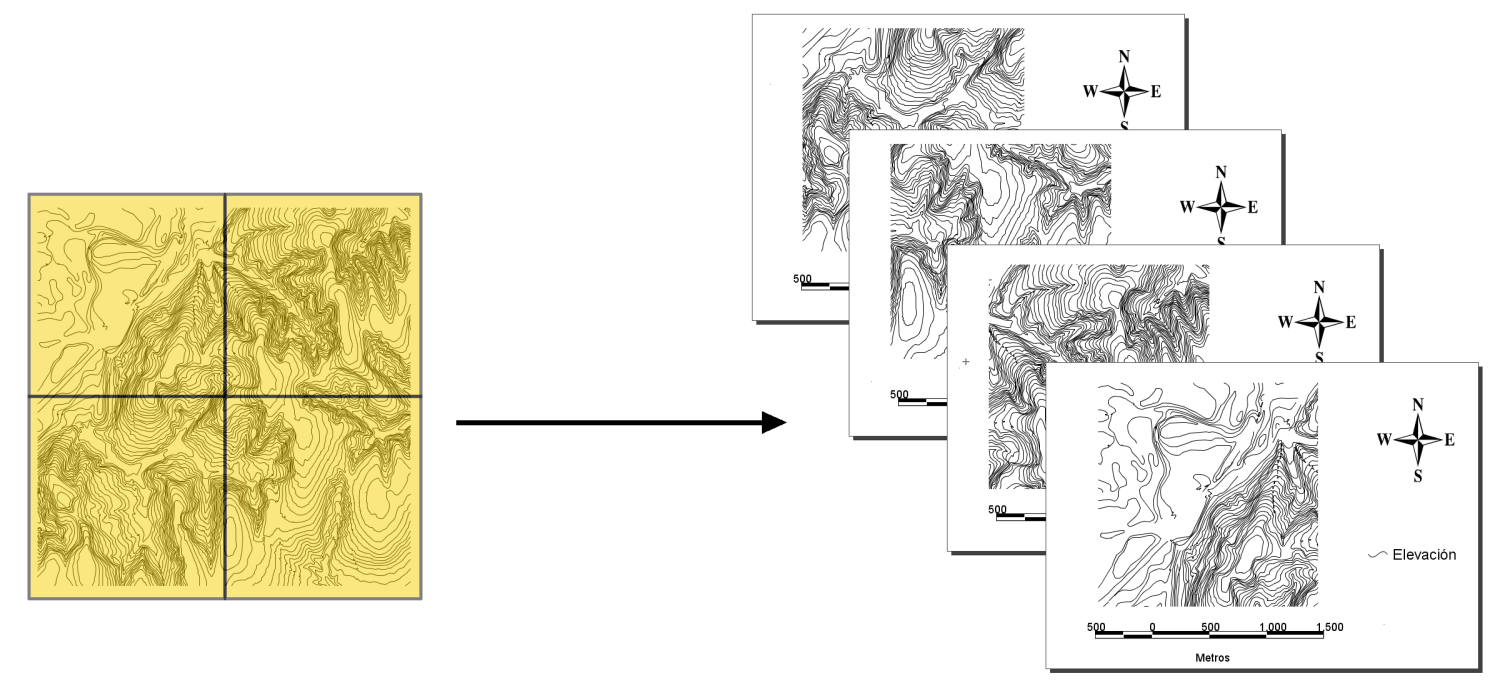
\includegraphics[width=.9\textwidth]{SIGs_escritorio/Serie_mapas.png}
\caption{\small La automatizaci�n de las tareas de creaci�n cartogr�fica permite simplificar la producci�n de grandes vol�menes de cartograf�a, como por ejemplo al dividir un �rea geogr�fica en una serie dada de mapas.}
\label{Fig:Serie_mapas} 
\end{figure}

Estas posibilidades surgen de la separaci�n existente en un SIG entre los datos espaciales y el dise�o del documento cartogr�fico que los contiene, del mismo modo que ya vimos existe entre datos y par�metros de representaci�n a la hora de visualizar los primeros.

\section{Tipos de herramientas de escritorio}

No todas las aplicaciones de escritorio presentan las anteriores funcionalidades de igual modo. Es frecuente que ciertos Sistemas de Informaci�n Geogr�fica tengan una fuerte componente de an�lisis, pero que otras de las funciones principales, como por ejemplo la edici�n, no se presenten tan desarrolladas. 

Un caso particular es el de aquellos SIG de escritorio que centran la gran mayor�a de sus capacidades en el terreno de la visualizaci�n, permitiendo un uso de los datos geogr�ficos similar al que corresponde a un mapa cl�sico, donde el trabajo con este se basa fundamentalmente en el an�lisis visual. 

Comenzaremos por estos �ltimos para dar un breve repaso a los principales tipos de aplicaciones de escritorio en funci�n de sus capacidades.

\subsection{Visores y exploradores}\label{VisoresYExploradores}

Las aplicaciones SIG de escritorio cuya funci�n principal es la visualizaci�n se conocen generalmente como \emph{visores} o \emph{exploradores}, y en la actualidad representan una fracci�n importante del conjunto total de herramientas SIG de escritorio. \index{Visor}\index{Explorador}

En ocasiones, se trata de aplicaciones en el sentido habitual, las cuales presentan capacidades reducidas de an�lisis y edici�n, y cuyo objetivo no es otro que el permitir la visualizaci�n de cartograf�a, sin incorporar las restantes posibilidades del SIG. En otros casos, son versiones simplificadas de soluciones SIG de escritorio m�s complejas, desarrolladas como alternativas m�s asequibles (en t�rminos de dificultad de manejo y aprendizaje, y tambi�n a veces en t�rminos de coste).

Una forma tambi�n habitual en la que se presentan los exploradores son como herramientas de apoyo a unos datos espaciales particulares. Para entender este tipo de enfoque, debe pensarse que un mapa cl�sico puede visualizarse de igual modo con independencia del uso que se le pretenda dar y de la experiencia y formaci�n de quien lo usa. Con un conjunto de datos espaciales en forma de una o varias capas, no sucede lo mismo, ya que estos datos no son un elemento <<visual>> de por s�. Es necesario utilizar un SIG para poder visualizarlos.

Un usuario experimentado no encontrar� problemas en manejar un SIG de escritorio complejo, pero un usuario con poca experiencia que lo �nico que desee sea <<ver>> la cartograf�a y explorarla visualmente (del mismo modo que un excursionista casual puede querer emplear un mapa topogr�fico) encontrar� el entorno de ese SIG demasiado complejo y con elementos que, en su mayor�a, no le son necesarios. Con la disponibilidad creciente de cartograf�a y la popularizaci�n de las tecnolog�as SIG, este tipo de usuarios ha crecido notablemente, y las aplicaciones adaptadas a sus necesidades han ido apareciendo y populariz�ndose igualmente de forma progresiva.

As�, existen visores que ocupan un papel secundario como parte de un producto compuesto que incluye al propio programa y a los datos en s�. Ejemplos muy claros y muy populares son aplicaciones como Google Earth (ver p�gina \pageref{GoogleEarth} y figura \ref{Fig:GEarth}), que permite que cada usuario incorpore su propia informaci�n para visualizar esta, pero cuyo mayor inter�s es el acceso a una enorme base de datos de im�genes de sat�lite con cobertura global. De esta forma, la aplicaci�n puede utilizarse para explorar una �rea deseada, sin necesidad de disponer junto con ella de datos para dicha zona, puesto que por defecto la aplicaci�n accede a una base de datos de im�genes que van indisolublemente unidos a ella.\index{Google!Earth}

\begin{figure}[!hbt]
\centering
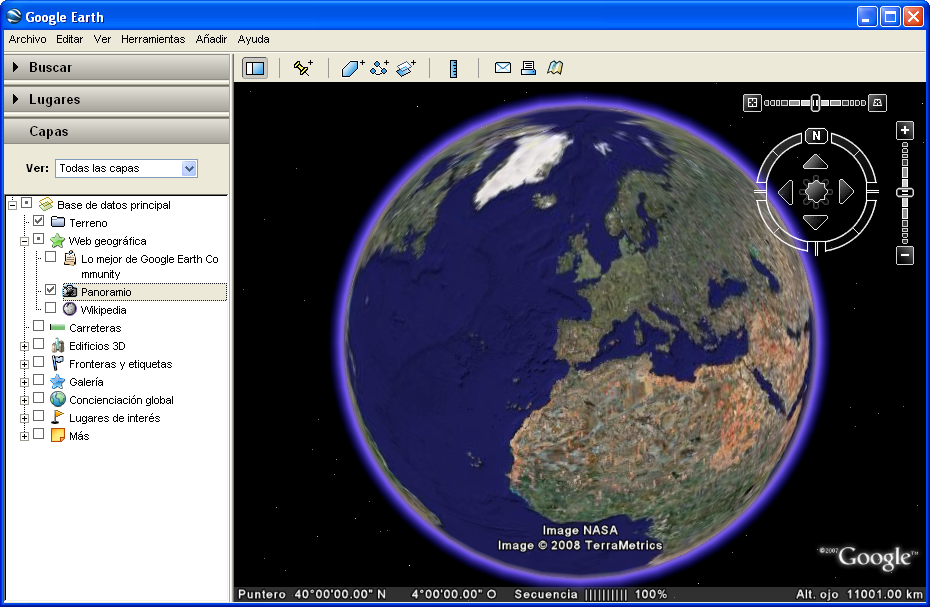
\includegraphics[width=.8\textwidth]{SIGs_escritorio/gearth.png}
\caption{\small Aspecto de un globo o visor tridimensional (GoogleEarth).}
\label{Fig:GEarth} 
\end{figure}

El usuario puede tambi�n a�adir sus propias capas y usar estos visualizadores de la misma manera que emplea las capacidades de visualizaci�n de un SIG de escritorio m�s rico en funcionalidades, pero parte del inter�s de la aplicaci�n no est� solo en sus capacidades, sino en los datos que tiene vinculados y que permiten emplear estas.

En otros casos, un organismo o empresa puede generar un conjunto de capas bien a partir de alg�n tipo de an�lisis o de cualquier otra metodolog�a, y opta por distribuir estas acompa�adas de un visor que permita un primer acceso a los datos. Todas esas capas podr�n ser empleadas dentro de un SIG que soporte los formatos de archivo en el que estas se hayan almacenado, pero aquellos usuarios que no dispongan de un SIG podr�n igualmente efectuar consultas b�sicas y explorar la cartograf�a haciendo uso del visor incorporado.

En l�neas generales podemos enumerar las siguientes caracter�sticas de los visores:

\begin{itemize}
	\item Interfaz simple en la que tienen un peso mayoritario las herramientas de navegaci�n.
	\item Capacidades de lectura de datos, pero no de escritura.
	\item Reducidas o nulas capacidades de edici�n y an�lisis.
	\item Enfocadas a usuarios no especializados.
\end{itemize}

Encontramos dos grupos b�sicos de visores, en funci�n de qu� tipo de visualizaci�n principal incorporan: planos y tridimensionales (globos). Mientras que una aplicaci�n SIG de escritorio completa puede presentar los dos tipos de representaci�n, y sobre ambas implementar las restantes funcionalidades tales como la edici�n o el an�lisis (aunque, como ya dijimos, en mayor proporci�n sobre las vistas bidimensionales), los visores habitualmente reducen sus capacidades de representaci�n a una de estas variantes.

Los visores bidimensionales, aunque sin alcanzar el enfoque especializado de una aplicaci�n completa, se orientan m�s al usuario con cierto conocimiento del �mbito SIG, mientras que la tendencia en los tridimensionales es a ofrecer herramientas de acceso a datos geogr�ficos con una apariencia atractiva. Ello, no obstante, no implica que estos visores carezcan de utilidad en el �mbito cient�fico, siendo igualmente herramientas v�lidas para todo tipo de investigaci�n o trabajo que incorpore cierta componente geogr�fica. De hecho, la popularizaci�n de este tipo de visores ha supuesto un gran acercamiento de los datos geogr�ficos y las capacidades SIG a toda una amplia comunidad de usuarios, incluyendo los del mundo cient�fico, permiti�ndoles realizar sus trabajos de forma m�s adecuada. Esto es especialmente cierto con aquellos visores que se hallan vinculados a bases de datos particulares, como ya se ha comentado, ya que permiten explotar los datos de dichas bases y proporcionar a todo usuario un sustrato de informaci�n geogr�fica sobre la que trabajar.


\subsection{Soluciones de escritorio completas}

La aplicaci�n SIG m�s habitual, y la que constituye la herramienta b�sica para el desarrollo de un proyecto SIG, es aquella que re�ne en un �nico producto todas las funciones b�sicas que hemos visto en este cap�tulo. Con las l�gicas diferencias en cuanto al grado de funcionalidad de estas seg�n el enfoque de la aplicaci�n, una aplicaci�n SIG de escritorio completa debe permitir la lectura de los datos, la creaci�n y modificaci�n de estos con sus capacidades de edici�n, su visualizaci�n, la realizaci�n de an�lisis con ellos y la generaci�n de resultados cartogr�ficos ya sea a partir de los datos originales o de datos generados en los procesos de an�lisis. Con todas estas capacidades, una herramienta SIG de escritorio constituye una soluci�n completa para todo tipo de proyectos SIG, y puede dar respuesta a todas las necesidades que en ellos se presentan.

Como ya vimos en el cap�tulo introductorio de esta parte, y tambi�n en el cap�tulo \ref{Bases_datos} dedicado a las bases de datos, la forma de abordar la implementaci�n de las distintas capacidades ha ido variando a medida que se iban desarrollando los SIG. En la actualidad, encontramos tanto SIG de escritorio que implementan en una sola aplicaci�n central todas las funcionalidades base, como grupos de aplicaciones muy interrelacionadas que implementan por separado cada una de dichas funcionalidades. Tanto en uno como en otro caso, existen elementos sobre los que las distintas herramientas del SIG se apoyan, especialmente en lo relativo al acceso a datos. %Veremos m�s sobre ellos en el cap�tulo \ref{Otros_tecnologia} dentro de esta misma parte.

Pese a que incorporan toda la gama de funcionalidades base, las soluciones de escritorio completas no cubren las necesidades de todo usuario de SIG. La convergencia a la que tienen este tipo de aplicaciones, comentada en el cap�tulo introductorio de esta parte del libro, no ha sido, como ya entonces se mencion�, completamente lograda en la actualidad. El problema no es ya un problema de integraci�n de tecnolog�as, sino una dificultad relativa a la gran amplitud de la ciencia de los SIG. Resulta imposible reunir en una sola herramienta todas las capacidades que un SIG de escritorio puede incluir, y es por ello que todas las soluciones de escritorio presentan alg�n tipo de especializaci�n, dando prioridad a alg�n �rea respecto a las restantes.

Una divisi�n que perdura, aunque en mucho menor medida que en los primeros SIG, es la existente entre SIG r�ster y SIG vectoriales, especialmente en lo relativo al an�lisis. Un usuario que trabaje con datos espaciales como los correspondientes, por ejemplo, a informaci�n catastral, utilizar� para su labor un SIG de escritorio distinto al que usara alguien cuyo trabajo implique mayoritariamente la realizaci�n de an�lisis del terreno o la creaci�n de modelos geogr�ficos, a pesar de que ambas soluciones probablemente incorporen capacidades tanto en el �mbito r�ster como en el vectorial. El alcance de estas, no obstante, ser� distinto en cada caso.

Incluso en caso de presentar una orientaci�n principalmente hacia los datos de tipo r�ster, existen tambi�n enfoques distintos dependiendo principalmente del tipo informaci�n que se vaya a manejar. Una divisi�n fundamental es la existente entre aquellas aplicaciones destinadas al manejo de im�genes y aquellas cuyo elemento principal de trabajo son las capas r�ster con otro tipo de valores, tales como MDE o capas similares.

Las im�genes, especialmente si se trata de im�genes de sat�lite, van a constar de una serie de bandas\index{Bandas} cuyo n�mero puede ser muy elevado, lo que requiere unas herramientas particulares para su manejo. Asimismo, gran parte de las funciones que vimos en el cap�tulo \ref{Procesado_imagenes} tales como las relativas a la correcci�n de im�genes, no tienen aplicaci�n para otro tipo de capas (no tiene sentido aplicar una correcci�n geom�trica a un MDE o una capa de pendientes, ya que estos datos necesariamente provienen de fuentes ya conveniente corregidas), por lo que en cierto modo pueden considerarse especificas de este campo, el de las im�genes, si bien es cierto que se trata de un campo de gran amplitud.\index{Modelo Digital del Terreno}

Por el contrario, capas como el propio MDE u otras similares solo contienen una �nica banda, y el tipo de operaciones que se desarrollan sobre ellos es bien distinto. Con objeto de simplificar estas operaciones, la estructura de estas aplicaciones ha de enfocarse hacia alguna de estas variantes, d�ndole prioridad sobre la otra. Por ello, las herramientas de escritorio que se orientan al trabajo con im�genes incorporan en general pocas o nulas herramientas en �reas como el an�lisis del terreno, mientras que aquellas que s� tratan estos an�lisis no incluyen salvo las funciones m�s simples para el manejo de im�genes (realces, ajuste de contraste, etc.), pero no las m�s espec�ficas.

En realidad, una aplicaci�n de escritorio global que cubriera todas estas funcionalidades no ser�a pr�ctica desde el punto de vista de su uso, pues ser�a excesivamente compleja. Es poco probable, igualmente, que un mismo usuario requiera un entorno profesional productivo en todas ellas, y m�s habitual sin embargo que centre su trabajo en un �rea concreta.

\section{Resumen}

Las herramientas de escritorio son la forma m�s cl�sica de los SIG. Entendemos como tales a aquellas herramientas ciertamente complejas que permiten llevar a cabo las tareas b�sicas de un SIG en sentido tradicional, como son el manejo de datos espaciales y el trabajo con los mismos. 

Podemos distinguir cuatro funcionalidades b�sicas que aparecen representadas en mayor o menor medida en un SIG de escritorio: visualizaci�n, edici�n, an�lisis y generaci�n de cartograf�a.

En funci�n del grado de desarrollo e implementaci�n en que las anteriores funcionalidades se encuentren en un SIG de escritorio, distinguimos distintas formas de estas herramientas. La divisi�n m�s gen�rica es aquella que distingue las herramientas pensadas para un trabajo completo en todas las distintas fases de un proyecto SIG de aquellas orientadas a la representaci�n y exploraci�n visual de los datos geogr�ficos. Estas �ltimas representan un enfoque m�s reciente, y en la actualidad est�n contribuyendo de manera muy notable a la expansi�n de las tecnolog�as SIG fuera del �mbito m�s especializado.

%\bibliographystyle{unsrt}
%\bibliography{../../Libro_SIG}
\chapter{Servidores remotos y clientes. \emph{Web Mapping}}\label{Servidores_y_clientes_remotos}

\chapterauthor{Olaya, V�ctor; Turton, Ian; Fonts, Oscar}

\begin{keypoints}
�C�mo se puede hacer que la informaci�n de un SIG se utilice en una red local o en Internet? $\bullet$ �C�mo se puede acceder a esa informaci�n?$\bullet$�Qu� entendemos por servicio?$\bullet$�C�mo aprovechan los SIG las capacidades de la red?$\bullet$�Por qu� la cartograf�a Web supone una gran revoluci�n en el �mbito SIG?$\bullet$�Qu� tipos de mapas podemos encontrar en la red?$\bullet$
\end{keypoints}

\bigskip

\begin{intro}
El avance de las redes locales y de Internet ha permitido que se acceda a la informaci�n geogr�fica contenida en un SIG utilizando el paradigma cliente--servidor. Para ello es necesario contar con componentes en el lado servidor que distribuyan la informaci�n y componentes en el lado del cliente para acceder a esta. En este cap�tulo veremos las caracter�sticas de ambos elementos y c�mo estos responden a las necesidades que el trabajo con datos remotos plantea en el �mbito SIG. Enfocaremos particularmente el cap�tulo a las tecnolog�as de \emph{Web Mapping}, las cuales permiten incorporar las ideas de los SIG dentro de paginas Web, utilizando un navegador Web como aplicaci�n principal. \index{Web Mapping}
\end{intro}

\section{Introducci�n}

Del mismo modo que podemos acceder a otros tipos de informaci�n a trav�s de Internet o de una red local, tambi�n podemos emplear esta para acceder a informaci�n geogr�fica y trabajar con ella dentro de un SIG. En el contexto actual, no puede dependerse en un SIG �nicamente de datos locales en forma de archivos en el mismo ordenador en el que se trabaja, sino que es necesario poder operar con datos remotos. Las redes son la v�a para la difusi�n de todo tipo de informaci�n, entre ella la informaci�n geogr�fica.

Los datos espaciales pueden ofrecerse a trav�s de una red de la misma manera que se ofrecen otro tipo de datos como im�genes o texto en una pagina Web. Para que en este proceso se maximicen las posibilidades que esos datos ofrecen, es necesario disponer de tecnolog�as adaptadas basadas en las tecnolog�as fundamentales de las redes, pero particularizadas al tipo de datos concreto que se maneja y los posibles usos que pueden darse.

Estas tecnolog�as son variadas y, como cabe esperar, han evolucionado paralelamente a otras basadas en la Web, a�adiendo progresivamente elementos tales como una mayor interactividad o flexibilidad Web. Las p�ginas est�ticas que formaban Internet hace unos a�os, muy limitadas en cuanto a sus posibilidades, han dado paso a lo que hoy se conoce como Web 2.0, donde encontramos \emph{blogs}, \emph{wikis} y otros tipos de p�ginas Web con capacidades mucho mayores y que permiten al usuario un trabajo muy distinto.\index{Interactividad}

Una evoluci�n similar han seguido las aplicaciones de la Web relacionadas con la informaci�n geogr�fica, habiendo ganado d�a tras d�a en riqueza hasta el estado actual donde pueden llegar a ofrecer casi tantas funcionalidades como un SIG de escritorio. Los mapas est�ticos que constitu�an los primeros elementos con componente geogr�fica en la Web han evolucionado hasta verdaderas aplicaciones que pueden convertir un navegador Web en una plataforma SIG completa. En su avance, las tecnolog�as Web van tomando elementos que ya conocemos de los SIG de escritorio, con objeto de trasladar toda su potencia al entorno de Internet, y uni�ndola as� con las capacidades que la red tiene como espacio com�n de actividad y conocimiento.

Aunque el objetivo final sea trasladar los SIG de escritorio a la red, las tecnolog�as necesarias distan bastante de las tecnolog�as SIG en sentido cl�sico, de la misma forma que, aun trabajando con un tipo de datos similar, un procesador de textos se diferencia mucho de un navegador Web. 

Fundamentalmente, estas tecnolog�as Web han de responder a dos necesidades principales: servir un elemento a trav�s de la red y tomar este para emplearlo. Es decir, tomar y recibir el elemento que es objeto de inter�s. Distinguimos as� los conceptos de \emph{servidor} y \emph{cliente}, que debemos ver con algo m�s detalle antes de continuar.\index{Servidor}\index{Cliente}

\section{�C�mo funciona Internet?}

Estamos acostumbrados a utilizar Internet a trav�s de aplicaciones tales como navegadores Web, y en muchos casos desconocemos c�mo se realiza ese proceso tan cotidiano hoy en d�a. Los fundamentos que residen detr�s de la consulta de una simple p�gina Web son esencialmente los mismos que vamos a encontrar para el caso de las tecnolog�as SIG en la red, por lo que es necesario conocerlos al menos someramente para poder entender el proceso que tiene lugar cuando empleamos una tecnolog�a SIG en Internet.

Cuando consultamos una p�gina Web existen tres elementos fundamentales que entran en juego: la propia red que hace de nexo entre sus elementos, nuestro ordenador que es el que realiza la petici�n de consulta, y la m�quina donde se encuentra almacenada esa p�gina que queremos consultar.

Conocemos como \emph{servidor} al elemento encargado de \emph{servir} alg�n tipo de contenido. En el �mbito SIG, se trata fundamentalmente (aunque no con car�cter exclusivo) de datos geogr�ficos, que constituyen el principal producto que se distribuye a trav�s de la red dentro de nuestro campo. En el ejemplo anterior, la m�quina que contiene la p�gina de inter�s es el servidor. Tambi�n se conoce como servidor el programa que, residiendo en esa m�quina, interpreta la petici�n y la procesa, sirviendo as� la p�gina.

El \emph{cliente} es responsable de \emph{pedir} ese dato al servidor, tomarlo y trabajar con �l. Nuestro navegador Web es el cliente en este caso, ya que es el que realiza la petici�n. Para ello, basta con introducir la direcci�n Web\footnote{T�cnicamente, una direcci�n Web como esta se conoce como URL (Uniform Resource Locator\footnote{Ver RFC 1738 \ref{RFC1738}})} correspondiente en la barra de direcciones del navegador. Al hacer esto, proporcionamos una serie de datos que son los que se emplean para realizar el proceso, y que vamos a ver a continuaci�n en detalle.\index{URL}

Supongamos la direcci�n Web \texttt{http://wiki.osgeo.org/wiki/Libro\_SIG}, en la cual puedes encontrar informaci�n relacionada con este libro e incluso descargarlo. Si visitas esa p�gina est�s efectuando una petici�n a trav�s de esa URL, la cual se compone de las siguientes partes:

\begin{itemize}
	\item \texttt{http:} El protocolo a usar, que define la forma en que se van a comunicar cliente y servidor. Aunque este es el m�s habitual, existen muchos otros tales como \texttt{ftp} o \texttt{mailto}. Puede encontrarse m�s acerca de estos protocolos en \cite{protocolosWeb}.
	\item \texttt{wiki.osgeo.org} Esta cadena identifica la m�quina donde reside la p�gina que buscamos. Es en realidad una versi�n m�s legible para el ojo humano de un c�digo num�rico que indica la direcci�n concreta. El navegador lo convierte en realidad en algo como 128.118.54.228.
	\item \texttt{wiki/Libro\_SIG} La p�gina que buscamos dentro de todas las que hay en esa m�quina. Se expresa como una ruta a partir del directorio ra�z del servidor, que no es necesariamente el directorio ra�z de la maquina servidora.
\end{itemize}
\index{FTP}

El proceso mediante el que podemos ver esa p�gina en un navegador Web comprende los cuatro pasos siguientes:

\begin{enumerate}
	\item El cliente realiza la petici�n.
	\item La petici�n se conduce a trav�s de la red hasta el servidor.
	\item El servidor busca la p�gina y la devuelve a trav�s de la red en caso de encontrarla, o devuelve una pagina de error en caso de no tenerla.
	\item El cliente recibe la p�gina y la representa.
\end{enumerate}


La figura \ref{Fig:Asi_funciona_internet} muestra un esquema de este proceso.

\begin{figure}[!hbt]   
\centering
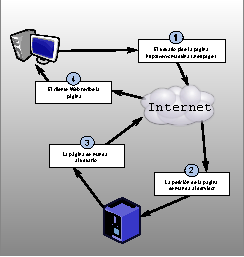
\includegraphics[width=.95\mycolumnwidth]{Servidores_y_clientes_remotos/Asi_funciona_internet.pdf}
\caption{\small Esquema del proceso de consulta de una p�gina Web desde un navegador.}
\label{Fig:Asi_funciona_internet} 
\end{figure}

\section{El valor de las tecnolog�as SIG Web}

Antes de abordar la parte m�s t�cnica de las tecnolog�as Web SIG, veamos el significado de estas y la funci�n que cumplen. Entenderemos en este contexto como tecnolog�as Web SIG a todos aquellos elementos que permiten la representaci�n de cartograf�a como un contenido m�s de una p�gina Web. Esto es lo que se engloba bajo la denominaci�n gen�rica de \emph{Web Mapping}.

Aunque este cap�tulo est� dedicado a las tecnolog�as Web dentro del �mbito SIG, y estas incluyen tanto servidores como clientes, las formas en las que se presentan los elementos del \emph{Web Mapping} dependen fundamentalmente del cliente, el cual es en general un simple navegador. 

Como vimos en el cap�tulo dedicado a los SIG de escritorio, estos pueden acceder a datos remotos, y para ello necesitan realizar una petici�n a un servidor siguiendo el esquema que hemos visto en el apartado anterior. Una vez que los datos est�n en el SIG (es decir, el servidor ha devuelto a este los datos que hab�a pedido), podemos operar con ellos usando las herramientas que ya conocemos.

En un entorno Web \emph{sensu stricto} tal como el de un navegador, las posibilidades son, no obstante, distintas, pues se trata de combinar los elementos cartogr�ficos con los restantes elementos que forman parte habitual de una p�gina Web. Las tecnolog�as Web de corte SIG se han desarrollado principalmente para su trabajo dentro de un navegador, es decir, como una alternativa a los SIG de escritorio o para alcanzar �reas nuevas en el trabajo con informaci�n geogr�fica digital. Su incorporaci�n en los SIG de escritorio aumenta las capacidades de estos, pero la principal potencia de estas tecnolog�as surge cuando se unen a otras funcionalidades de tipo Web.

En resumen, el objetivo b�sico que pretenden cumplir las tecnolog�as que vamos a ver, especialmente las del lado del cliente, es llevar las funcionalidades de un SIG a la Web, para as� compartir la potencia de ambos componentes.  Las ventajas de llevar el SIG a la Web en lugar de incorporar los elementos de esta �ltima en un SIG de escritorio tradicional son notables, y existen grandes diferencias entre las soluciones que se obtienen en ambos casos. Estas diferencias tienen que ver sobre todo con los usuarios y su perfil, as� como con el dise�o mismo de las aplicaciones. 

Mientras que un SIG de escritorio se orienta principalmente a usuarios m�s especializados, poder dotar a un sencillo navegador Web de capacidades de visualizaci�n o edici�n de informaci�n geogr�fica hace que estos lleguen a un p�blico distinto y abre nuevas posibilidades. Los usuarios avanzados encuentran igualmente utilidad en el \emph{Web Mapping}, que se complementa en muchos terrenos con los SIG de escritorio. Por su parte, los usuarios no especializados, desconocedores de otras tecnolog�as SIG, pueden incorporarse al �mbito SIG a trav�s de las tecnolog�as Web.

Algunas de las ideas fundamentales que caracterizan a las tecnolog�as de \emph{Web Mapping} y su papel actual son las siguientes:

\begin{itemize}
	\item No es necesario un software SIG espec�fico. Al menos, no es necesario desde el punto de vista del usuario, que no ha de instalar nada adicional en su ordenador. Acceder a cartograf�a remota e incluso a funcionalidades avanzadas basadas en esos datos no requiere m�s que un simple navegador Web, algo presente en cualquier ordenador hoy en d�a. La barrera que puede suponer el trabajar con una aplicaci�n espec�fica se diluye cuando incorporamos las capacidades de esta en algo tan habitual como un navegador.
	\item Perfil menos t�cnico. No solo las aplicaciones est�n pensadas para su utilizaci�n por parte de usuarios no especializados, sino que la incorporaci�n de estos al �mbito SIG hace que la cartograf�a deje de ser un elemento propio de esos usuarios m�s t�cnicos. Poniendo al alcance de todos las capacidades de edici�n y creaci�n de cartograf�a hace que cualquiera pueda generar su propia informaci�n geogr�fica no especializada y adem�s ponerla a disposici�n de otros usuarios.
	\item Potenciamiento del trabajo colaborativo. La red es un punto de encuentro que favorece de forma natural la colaboraci�n. Proyectos como la Wikipedia, posibles gracias a esta capacidad de  Internet para facilitar el trabajo com�n de m�ltiples personas, tiene sus equivalentes en el �mbito de la informaci�n geogr�fica. Los SIG dejan de ser algo personal reducido al �mbito de un ordenador o una peque�a red, para ser algo global en una red de muchos SIG interconectados. Y m�s importante que esto, los datos tambi�n se hacen globales, pudiendo ser empleados e incluso editados por todos.
	\item Informaci�n m�s actualizada, incluso en tiempo real. La Web es el canal ideal para transmitir la informaci�n de forma inmediata y flexible. A las ventajas de los datos digitales sobre los anal�gicos en este sentido, que ya vimos en el cap�tulo \ref{Introduccion_datos}, hay que sumar que la sencillez de acceso que aporta una interfaz Web hace todav�a m�s accesible la informaci�n geogr�fica m�s reciente.
	\item Independencia del sistema. Un mapa Web puede verse y usarse del mismo modo en cualquier ordenador, con independencia del sistema operativo, el navegador e incluso el dispositivo empleado (PC, PDA, etc.). Si este mapa se basa en est�ndares abiertos, la soluci�n es todav�a m�s interoperable, como veremos en el cap�tulo \ref{Estandares}.\index{Est�ndares}\index{PDA}
	\item Personalizaci�n de aplicaciones. Una de las tendencias m�s importantes en el �mbito del \emph{Web Mapping} es la creaci�n de aplicaciones que personalizan una base com�n para un determinado uso. Sobre una base compuesta por un juego de datos gen�rico (generalmente im�genes de sat�lite y mapas base tales como un mapa de carreteras) y una aplicaci�n SIG, se crean peque�as aplicaciones de forma sencilla, a las cuales se pueden a�adir de modo tambi�n simple nuevos datos. Estas aplicaciones se conocen como \emph{mashups}, y una vez creadas puede incorporarse a una p�gina Web distinta. Dedicaremos una secci�n completa de este cap�tulo a desarrollarlas en detalle.\index{Mashup}
	
	Mediante uno de tales \emph{mashups}, un usuario puede crear, sin excesivos conocimientos sobre SIG, una aplicaci�n particular que ponga sobre ese juego de datos general los emplazamientos de, por ejemplo, todos aquellos que visitan su p�gina Web. Las posibilidades en este sentido son pr�cticamente infinitas, y proliferan de forma exponencial en Internet.
	\item Combinaci�n de cartograf�a y otros elementos. Si llevamos las capacidades SIG a un navegador, adem�s de estas dispondremos en ese navegador de muchas otras posibilidades, tales como la representaci�n de elementos multimedia (v�deo, sonido, etc.) o el uso de hiperenlaces. El navegador es hoy en d�a la aplicaci�n vers�til por excelencia, y ello hace que podamos a�adir a las capacidades SIG una larga serie de otras funcionalidades no relacionadas directamente con la informaci�n geogr�fica, y no presentes en su mayor�a en los SIG de escritorio.
\end{itemize}

La importancia de las tecnolog�as Web se debe, por tanto, principalmente a un raz�n social y no a una tecnol�gica, aunque es innegable que las tecnolog�as novedosas que se desarrollan en este campo aportan al �mbito SIG posibilidades antes desconocidas. Estas nuevas posibilidades enriquecen notablemente los SIG de escritorio si estos implementan las capacidades de acceso a datos remotos, ampliando el alcance de ese tipo de aplicaciones. Cuando se implementan, sin embargo, en un entorno puramente Web tal como en el seno de un navegador y se crea una p�gina Web con elementos SIG, se consigue ampliar el abanico de usuarios potenciales y as� tambi�n crecen las posibilidades y las formas en que el propio SIG puede presentarse.


\section{Formas de cartograf�a en la Web}

Las formas en las que pueden presentarse las tecnolog�as SIG dentro de un entorno Web var�an en cuanto a su similitud con los SIG de escritorio, incorporando m�s o menos elementos de los que son habituales en este tipo de aplicaciones. Como parece l�gico pensar, ha existido una evoluci�n progresiva, de tal modo que en la actualidad existen m�s elementos propios de los SIG de escritorio dentro de las tecnolog�as Web SIG, y la cartograf�a Web hoy en d�a permite realizar un trabajo m�s similar al que se desarrolla en un SIG cl�sico.

Una primera y sencilla clasificaci�n de los tipos de cartograf�a Web es la que divide esta en mapas \emph{est�ticos} y \emph{din�micos}\cite{Kraak2001Francis}. 

Un mapa est�tico es simplemente una imagen con informaci�n cartogr�fica, la cual no permite ning�n tipo adicional de trabajo con ella que no sea la mera observaci�n. En este sentido, se asemeja a un mapa cl�sico, donde el usuario no puede interactuar directamente con el contenido del mapa. A efectos de trabajo real, las posibilidades son a�n menores ya que acciones tales como mediciones tampoco pueden realizarse, ni siquiera con medios mec�nicos como el caso de un mapa en papel. Junto a esto, la resoluci�n de una pantalla com�n es mucho menor que la que presenta un mapa impreso, con lo que la calidad del mapa no es comparable.

Este tipo de mapas, por tanto, no responden a las funcionalidades que un SIG ha de tener para poder prestar utilidad en el manejo y uso de informaci�n geogr�fica, y difieren notablemente de un SIG de escritorio, incluso en la versi�n m�s b�sica y primitiva de estos �ltimos.

Incorporar este tipo de mapas a una p�gina Web no requiere ninguna tecnolog�a particular, y puede llevarse a cabo con elementos gen�ricos tanto del lado del cliente como del servidor, pues el dato realmente no es un dato geogr�fico como tal, sino una mera imagen (y esa imagen no va acompa�ada de informaci�n tal y como su sistema de referencia), algo para lo cual cualquier servidor o cliente actual ofrece soporte.

La figura \ref{Fig:XeroxPARC} muestra una imagen de una primigenia cartograf�a Web presentada a trav�s del visor Xerox PARC Map Viewer\index{Xerox PARC Map Viewer}.

\begin{figure}[!hbt]   
\centering
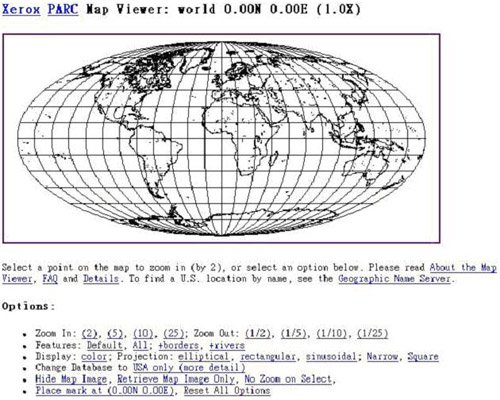
\includegraphics[width=.85\mycolumnwidth]{Servidores_y_clientes_remotos/XeroxPARC.png}
\caption{\small Visor de mapas Xerox PARC Map Viewer, uno de los primeros en su campo}
\label{Fig:XeroxPARC} 
\end{figure}


Por su parte, un mapa din�mico es aquel que no se compone de una imagen inm�vil, sino que esta var�a y se adapta en funci�n de los requerimientos del usuario o seg�n alguna serie de par�metros prefijados. De acuerdo con esto, los mapas din�micos pueden ser interactivos o no, dependiendo de si es el usuario quien directamente modifica la representaci�n del mapa.

Como ejemplo de mapa din�mico no interactivo podemos citar mapas animados que encuadran una determinada zona y muestran la variaci�n de una variable a lo largo del tiempo. Mapas de variables climatol�gicas o una serie animada de mapas que reflejan el avance de un incendio son ejemplos habituales de este grupo.

Tampoco en este tipo de mapas aparecen las funciones esperables en una aplicaci�n SIG, y una vez m�s no se requieren tecnolog�as espec�ficas para poder incorporar este tipo de elementos en una p�gina Web.

La interactividad es la que aporta las posibilidades necesarias para comenzar a incorporar funciones SIG a la cartograf�a Web, y sin ella no podemos hablar en realidad de tecnolog�as SIG puramente dichas.

La forma de interactividad m�s b�sica que se implementa en una p�gina Web en el trabajo con cartograf�a es la que permite la modificaci�n de la forma en que los datos geogr�ficos se visualizan. Las herramientas que permiten modificar la escala de visualizaci�n (acercarse o alejarse) y desplazar el mapa, las cuales ya nombramos como capacidades b�sicas en los SIG de escritorio, aportan a la cartograf�a Web muchas posibilidades nuevas. Entre ellas, es de destacar que mediante estas herramientas la extensi�n de los datos no se encuentra limitada por la propia extensi�n de la pantalla o la dimensi�n del navegador. 

Si se trabaja con im�genes est�ticas, trabajar con datos que cubran toda la extensi�n del globo implica hacerlo a una escala de muy poco detalle, pues ha de representarse toda la imagen de forma simultanea. Permitiendo que el usuario elija la escala de representaci�n y ajuste la extensi�n con la que se desea trabajar, un navegador Web se convierte en una ventana hacia datos que pueden tener cualquier extensi�n y volumen, y hacia el trabajo con ellos de forma din�mica e interactiva.

Esto es de especial importancia si pensamos que las m�quinas que se encuentran al otro lado (en el servidor) son ordenadores potentes con gran capacidad, que pueden almacenar enormes juegos de datos. Un juego de datos con im�genes de todo el mundo a gran resoluci�n ocupa un tama�o que probablemente lo haga inutilizable en un ordenador personal (adem�s de que ese juego probablemente quede fuera del alcance del usuario de ese ordenador en lo que a su adquisici�n respecta), pero puede perfectamente ser servido desde un potente servidor, sirviendo en cada caso la <<porci�n>> de �l que cada usuario requiere seg�n utiliza el cliente correspondiente. En esto se basan gran parte de servicios y de aplicaciones desarrolladas sobre ellos, como veremos m�s adelante.

De especial importancia para el desarrollo de estas capacidades ha sido la popularizaci�n y mejora de las tecnolog�as que permiten el desarrollo de las denominadas \emph{Aplicaciones Ricas de Internet} (RIA)\footnote{Rich Internet Applications}. Este tipo de aplicaciones llevan a la Web algunos elementos de las tecnolog�as de escritorio, y en general permiten optimizar el volumen de datos necesario para operar con la aplicaci�n dentro del entorno del navegador.\index{Rich Internet Applications (RIA)}

Si no se emplean estas tecnolog�as, un cambio m�nimo en la configuraci�n de la pagina por parte del usuario (por ejemplo, modificar el encuadre del mapa en una aplicaci�n SIG), requiere la recarga total de la p�gina, de la misma forma que sucede cuando hacemos clic en un hiperenlace. En realidad, estamos pasando a una p�gina Web distinta. 

En un entorno RIA, sin embargo, se cargan al inicio (en el primer acceso a la p�gina) los elementos que constituyen la aplicaci�n en s�, y posteriormente se transmiten �nicamente los datos que vayan siendo necesarios a medida que el usuario opere con la aplicaci�n. Esto mejora notablemente la sensaci�n del usuario, ya que este nunca tiene ante s� una pantalla sin contenido mientras se carga la p�gina, puesto que esta ya no ha de cargarse de nuevo, y la carga de datos puede adem�s realizarse mientras el propio usuario opera.

AJAX \footnote{Asynchronous JavaScript And XML} \cite{garrett2005ajax} es una t�cnica de desarrollo muy popular en este sentido, y de la que los SIG Web hacen uso habitualmente. La figura \ref{Fig:AJAX} muestra una comparaci�n entre el esquema de una aplicaci�n Web tradicional y una basada en AJAX. \index{AJAX}

\begin{figure}[!hbt]   
\centering
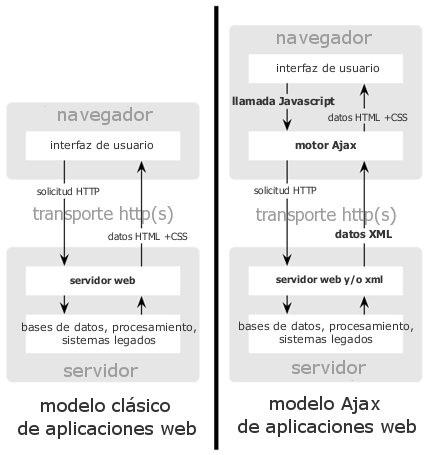
\includegraphics[width=.45\mycolumnwidth]{Servidores_y_clientes_remotos/ajax.png}
\caption{\small Comparaci�n entre el esquema de una aplicaci�n Web tradicional y una basada en AJAX.(adaptado de \cite{garrett2005ajax}).}
\label{Fig:AJAX} 
\end{figure}

Profundizar m�s en estos aspectos es, no obstante, demasiado t�cnico para el enfoque de este libro, no siendo necesario adem�s para la comprensi�n de las tecnolog�as Web desde el punto de vista del usuario. Tan solo es necesario diferenciar entre el comportamiento de una p�gina Web anterior a la introducci�n de estas t�cnicas, en la cual cualquier interacci�n (clic del rat�n) supon�a una recarga completa de la p�gina, mientras que en el caso de una RIA, la experiencia es m�s fluida y cercana a la que se tiene usando una aplicaci�n de escritorio.

\begin{figure}[!hbt]   
\centering
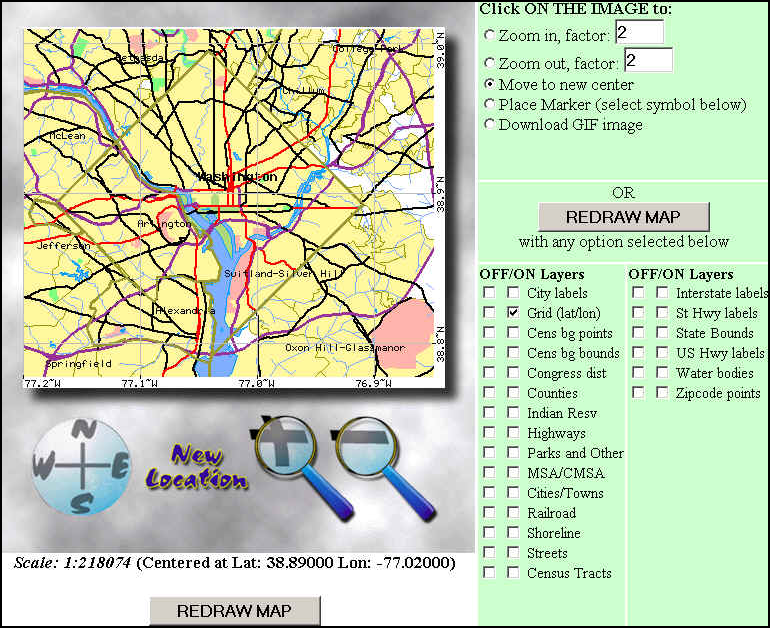
\includegraphics[width=.9\mycolumnwidth]{Servidores_y_clientes_remotos/tiger.png}
\caption{\small Interfaz de TIGER MapServer (a�o 1997)}
\label{Fig:Tiger} 
\end{figure}


La figura \ref{Fig:Tiger} muestra el aspecto de una aplicaci�n de \emph{Web Mapping} previa a la introducci�n de tecnolog�as como AJAX, en particular la Web a trav�s de la que se acced�a a los datos del proyecto TIGER, creado por el U.S Census Bureau.\index{TIGER}\index{U.S. Census Bureau}


Adem�s de modificar la zona representada, un usuario debe poder modificar la forma en que los datos dentro de esa zona se muestran. Es decir, debe poder cambiar el estilo de los elementos representados, variando colores o formas de la misma manera que esto puede hacerse en un SIG de escritorio. Asimismo, muchas aplicaciones Web permiten la consulta de varias capas de datos, incluso de datos provenientes de varios servidores distintos, datos que no necesariamente han de mostrarse todos simult�neamente. Igual que en un SIG de escritorio seleccionamos unas u otras capas para su visualizaci�n y podemos alterar el orden de representaci�n de estas, tambi�n podemos realizar estas operaciones en una aplicaci�n SIG Web.

Esto hace que una aplicaci�n SIG dentro de un navegador se convierta en una herramienta completa para el acceso a uno o varios juegos de datos remotos cuyo contenido es abundante (no solo en extensi�n sino tambi�n en tipos de datos suministrados), ya que permite una gran configurabilidad y deja en manos del cliente (esto es, del usuario), la forma de tomar esos datos y mostrarlos.

Las capacidades de edici�n tambi�n tienen lugar en los SIG Web, ampliando las posibilidades que la interactividad m�s b�sica ofrece. Un usuario puede a�adir su propia informaci�n a un SIG Web o bien modificar una capa existente empleando su navegador. Las tecnolog�as SIG siguen en este sentido a las tecnolog�as Web m�s generales, adoptando los conceptos de la Web 2.0 y ampliando las posibilidades de los usuarios de colaborar directamente en los contenidos de la red. Por ejemplo, \emph{OpenStreetMap} \cite{webOSM} es un sitio equivalente a la bien conocida Wikipedia, en el cual los usuarios pueden a�adir sus propias descripciones de elementos geogr�ficos que ellos mismos definen.\index{Wikipedia}\index{OpenStreetMap}

A estas mismas tecnolog�as se les puede dar usos m�s restringidos sin que necesariamente sea dentro de un proyecto colaborativo abierto. Por ejemplo, una administraci�n local puede dar acceso a los propietarios de suelo para que puedan consultar su catastro, mediante un sistema de autenticaci�n conveniente, incluso editar informaci�n de sus parcelas. Est� informaci�n puede ser de tipo no espacial (es decir, los l�mites de las parcelas ser�an fijos), ya que las capacidades de edici�n no han de limitarse a la componente espacial.\index{Autenticaci�n}

Por �ltimo, y aunque en la actualidad son pocos los servicios de este tipo que existen, y no pueden compararse las prestaciones con las que ofrecen los SIG de escritorio, la cartograf�a Web puede ofrecer herramientas de an�lisis. Adem�s de representar un conjunto de datos geogr�ficos y permitir al usuario navegar en ellos e incluso editarlos, pueden extraerse resultados a partir de esos datos. 

Un tipo de aplicaci�n bastante extendida de este tipo es el c�lculo de rutas �ptimas. A partir de una capa con v�as de comunicaci�n un usuario establece un punto de salida y otro de destino y la aplicaci�n Web calcula la ruta que optimiza el tiempo empleado o la distancia total recorrida, seg�n lo explicado en el cap�tulo \ref{Costes}. \cite{webGuiaCampsa} es un ejemplo de este tipo de aplicaciones en el cual la interfaz no es la de un SIG de escritorio habitual, sino que se introducen los lugares de origen y destino tecleando sus nombres y despu�s la ruta calculada se muestra sobre un mapa y tambi�n como un conjunto de indicaciones a seguir. Es decir, que sobre una base de c�lculo SIG se crea una aplicaci�n m�s completa que la que es habitual encontrar en un SIG, aprovechando la mayor riqueza de elementos que pueden utilizarse dentro de un navegador Web.

El t�rmino \emph{Web Mapping}, habitualmente empleado para designar a la cartograf�a Web, se sustituye por \emph{Web GIS} a medida que las capacidades de las aplicaciones Web aumentan, para indicar as� que todos los componentes que forman parte de un SIG en su sentido cl�sico, esto es, un SIG de escritorio, se incorporan a dicha aplicaci�n Web.\index{Web GIS}

La figura \ref{Fig:Tipos_Cartografia_Web} muestra un esquema de la evoluci�n de la cartograf�a Web a trav�s de los tipos anteriormente descritos.

\begin{figure}[!hbt]   
\centering
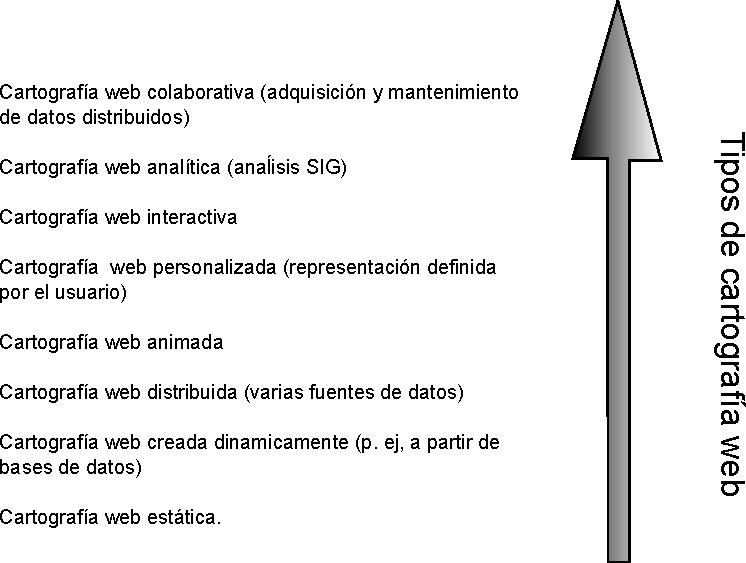
\includegraphics[width=.6\mycolumnwidth]{Servidores_y_clientes_remotos/tipos_cartografia_web.pdf}
\caption{\small Evoluci�n de los tipos de cartograf�a en la Web (seg�n \cite{Kraak2001Francis})}
\label{Fig:Tipos_Cartografia_Web} 
\end{figure}

\subsection{ \emph{Mashups}}

Se conoce como \emph{mashup} o \emph{aplicaci�n Web h�brida} a una aplicaci�n que basa sus contenidos en los de otras p�ginas Web, integr�ndolos y creando una nueva p�gina que ofrece un servicio distinto. Un \emph{mashup} accede a los servicios que otras p�ginas proporcionan de forma p�blica dando un uso distinto a estos en un nuevo contexto.\index{Mashup}\index{Aplicaci�n Web h�brida|see{Mashup}}

Por lo general, la creaci�n de un nuevo \emph{mashup} resulta sencilla, mucho m�s que lo que ser�a el desarrollo desde cero de esa misma aplicaci�n. Los \emph{mashups} suponen una extensi�n de los conceptos de la Web 2.0 al terreno de la programaci�n, ya que permiten una participaci�n mayor por parte de los usuarios en los contenidos de la propia Web. Si los blogs permiten hoy la publicaci�n de texto sin que sea necesario saber crear una p�gina Web, los \emph{mashups} hacen sencillo aportar a la Web contenidos interactivos en forma de nuevas aplicaciones, sin requerir unos elevados conocimientos de programaci�n o tecnolog�as Web a bajo nivel. \index{Web 2.0}

De este modo, los \emph{mashups} favorecen sobre todo la creatividad, y cuando una aplicaci�n Web pone sus servicios a disposici�n de otros para que los empleen en la creaci�n de alg�n tipo de \emph{mashup}, ello no va enfocado a programadores expertos, sino a cualquiera que sea capaz de tener una idea relevante para utilizar esos servicios y sea capaz de ponerla en pr�ctica. Tanto los servicios en s� como los datos en los que estos pueden basarse, y que son empleados para la creaci�n de un \emph{mashup}, alcanzan as� un p�blico mayor, rompiendo las barreras que anteriormente restring�an el uso de esas tecnolog�as a entornos profesionales especializados.

Los \emph{mashups} existen en todos los �mbitos de las aplicaciones Web, pero es en el �mbito SIG donde han adquirido una mayor importancia y en el que proliferan en mayor medida. Es por esto que resulta de inter�s tratarlos con algo m�s de profundidad, pues el impacto que est�n teniendo en la popularizaci�n de las tecnolog�as SIG es muy elevado.

Dos son las razones principales por las que los \emph{mashups} con componente SIG son tan populares:

\begin{itemize}
 \item La mayor�a de la informaci�n que encontramos en la Web puede georreferenciarse. Esto hace que una gran parte de los contenidos de una p�gina Web puedan complementarse con alg�n tipo de elemento geogr�fico, principalmente un visor de cartograf�a en el que poder mostrar esa informaci�n georreferenciada con la que se trabaja.
\item La informaci�n geogr�fica es de dif�cil acceso, especialmente a gran escala y por parte de usuarios o desarrolladores no especializados. Si el inter�s de a�adir a cualquier pagina Web alg�n elemento de tipo SIG resulta claro, tambi�n es cierto que suelen necesitarse datos adicionales con que acompa�ar a los propios datos de la p�gina. Es decir, si nuestra p�gina Web recoge informaci�n sobre restaurantes en la zona, mostrar la localizaci�n de esos restaurantes enriquecer� el contenido, aunque para que esta funcionalidad sea verdaderamente �til deberemos contar con alg�n tipo de mapa base (cartograf�a de calles, fotograf�a a�rea, etc.) que ayude al usuario a emplazar un restaurante dado o calcular la forma �ptima de llegar hasta �l.

Esta cartograf�a base implica un coste elevado, normalmente no asumible para un uso como este. Sin embargo, disponer de una cartograf�a base ofrecida por un proveedor que permita crear alg�n tipo de \emph{mashup} sobre ella facilita que existan este tipo de servicios, como as� lo atestigua el gran n�mero de distintas aplicaciones Web que se desarrollan de este modo.
\end{itemize}

De entre los muchos existentes en la actualidad, Google Maps \cite{webGoogleMaps} es el servicio m�s popular para la creaci�n de \emph{mashups}, y el que ha supuesto una verdadera revoluci�n en este sentido\index{Google!Maps}. Para ver algunos ejemplos relevantes de este tipo de sitios Web, puede consultarse la p�gina Web \cite{webGoogleMapsCaseStudies}, donde se recopila informaci�n sobre Google Maps y los \emph{mashups} m�s exitosos que derivan de este servicio.


\section{Clientes y servidores}

Ahora que conocemos algunas ideas generales sobre cartograf�a Web, veamos algo m�s en detalle los elementos tecnol�gicos que hacen posible su funcionamiento: los servidores y los clientes. Veremos en este apartado las funcionalidades que presentan y algo m�s de los fundamentos tecnol�gicos en los que se basan, que se apoyan sobre las ideas b�sicas de funcionamiento de Internet que ya vimos anteriormente.

En primer lugar, veamos algunas ideas b�sicas sobre la arquitectura cliente--servidor. De modo gr�fico, la relaci�n entre ambos elementos puede representarse seg�n la figura \ref{Fig:Servidores_y_clientes}. En ella, un n�mero variable de clientes se <<conectan>> a un servidor, del cual obtienen una serie de datos cuando este responde a las peticiones formuladas por cada uno de los clientes. En la arquitectura cliente--servidor, este �ltimo es el que posee la informaci�n a compartir a trav�s de los servicios, mientras que en cada uno de los clientes se almacena tan solo la informaci�n personal de estos.

\begin{figure}[!hbt]   
\centering
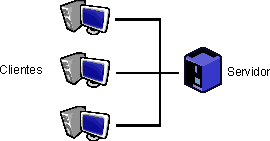
\includegraphics[width=0.65\mycolumnwidth]{Servidores_y_clientes_remotos/Servidores_y_clientes.pdf}
\caption{\small Relaci�n entre clientes y servidores.}
\label{Fig:Servidores_y_clientes} 
\end{figure}

En el sistema cliente--servidor se presentan las siguientes caracter�sticas principales:

\begin{itemize}
	\item El servidor brinda servicio a m�ltiples clientes. Los clientes, por su parte, tambi�n pueden acceder a servicios en varios servidores, aunque esa multiplicidad es mucho m�s relevante en el caso del servidor. Pi�nsese, por ejemplo, en un navegador Web con el que podemos acceder a varias p�ginas y un servidor de una de dichas p�ginas. Mientras que en el cliente no accedemos simult�neamente a un gran n�mero de p�ginas (si la pagina es est�tica solo usamos el servicio al cargarla, y no cargamos m�s de una capa en un instante dado), el servidor debe estar preparado para responder a muchas peticiones simultaneas y satisfacer la demanda de muchos clientes en un instante concreto.
	\item Los clientes no dependen de la ubicaci�n f�sica del usuario, el sistema operativo o la arquitectura f�sica de la m�quina. Esto es as� porque el cliente no necesita conocer la l�gica interna del servidor para usar sus servicios. Lo �nico necesario es que el servidor pueda exponer una interfaz externa que act�e como un modo de comunicaci�n para recibir las peticiones del cliente, siendo esta comunicaci�n siempre transparente para este �ltimo. 
	\item La carga de proceso se puede repartir entre cliente y servidor. En funci�n del servicio y de las capacidades del cliente, el trabajo puede dividirse de una u otra forma entre las partes implicadas.
\end{itemize}

\index{Cliente}\index{Servidor}\index{Carga de proceso}


\subsection{Servidores}\label{Servidores}
\index{Servidor}

El servidor es el elemento encargado de ofrecer el servicio como tal, respondiendo a las peticiones del cliente. A medida que los clientes se hacen m�s complejos y presentan mayor n�mero de funcionalidades, tambi�n los servidores deben ser capaces de proporcionar servicios m�s elaborados. Las capacidades fundamentales a las que responden los servidores dentro del �mbito SIG pueden dividirse en los siguientes grupos:

\begin{itemize}
\item Servir representaciones de los datos. Los servicios de cartograf�a Web, tanto en sus or�genes como en la actualidad, son eminentemente gr�ficos, y en �ltima instancia lo que la aplicaci�n Web correspondiente va a hacer es mostrarnos alg�n tipo de imagen con un mapa formado a partir de una serie de datos geogr�ficos. El servidor puede responder directamente a este tipo de necesidades, preparando una imagen a partir de los datos geogr�ficos de los que dispone. En el caso de que estos sean ya im�genes ---por ejemplo, im�genes de sat�lite u ortofotos---, bastar� servir estas, transmitiendo una versi�n escalada de las dimensiones exactas que el cliente necesite para representar en pantalla. En caso de que los datos sean de tipo vectorial, o bien r�ster sin una forma de representaci�n impl�cita ---por ejemplo, un Modelo Digital del Terreno--- es necesario emplear alg�n m�todo para asignarles dicha representaci�n. Este puede ser asignado por defecto por el servidor, que establecer� una simbolog�a fija, o bien ofrecer un servicio m�s complejo en el que el cliente no solo pide una representaci�n gr�fica de una serie de datos para una zona dada, sino que adem�s puede especificar \emph{c�mo} crear esa representaci�n.\index{Modelo Digital del Terreno}\index{Ortofotograf�a}

Asimismo, el servidor puede ofrecer la posibilidad de seleccionar los datos empleados para crear la representaci�n gr�fica. En t�rminos de un SIG de escritorio esto es equivalente a seleccionar qu� capas se van a representar de entre el total de las que se encuentran abiertas o bien en nuestro cat�logo de datos al que tenemos acceso desde el SIG. En el caso de un servicio Web, el servidor dispone de una serie de capas a las que puede acceder, y a la hora de servir una imagen puede preparar esta usando unas u otras seg�n las necesidades que el cliente especifique a la hora de hacer la petici�n del servicio. De igual modo, el orden en que se desea que las capas se pinten en el mapa tambi�n debe poder ser especificado por el cliente.

\item Servir los datos directamente. Una opci�n m�s flexible que lo anterior es que el servidor provea directamente los datos geogr�ficos y sea despu�s el cliente quien los utilice como corresponda, bien sea simplemente represent�ndolos ---en cuyo caso deber�a ser el propio cliente quien establezca la simbolog�a, ya que esta tarea ya no queda en manos del servidor--- o bien trabajando con ellos de cualquier otra forma, como por ejemplo analiz�ndolos. 

Aunque las posibilidades son mayores en este caso, se requieren por parte del cliente unas capacidades mayores, ya que mientras que representar una imagen es algo sumamente sencillo desde el punto de vista t�cnico, crear esta a partir de los datos geogr�ficos es m�s complejo.

\item Servir consultas. Un paso m�s all� en la funcionalidad que puede ofrecer el servidor es responder a \emph{preguntas} realizadas por el cliente relativas a los datos, ya sean estas relativas a la parte espacial de dichos datos, o bien a su componente tem�tica. El servidor puede ofrecer como respuesta conjuntos reducidos de los datos de los que dispone, o valores que describan a estos. Estas consultas pueden ser �tiles, por ejemplo, para establecer filtros previos cuando se dispone de un conjunto amplio de or�genes de datos. Un cliente Web puede obtener datos de distintos servidores, y puede consultar si, para un zona dada, estos servidores disponen de informaci�n, sin m�s que consultar la extensi�n cubierta por los datos de cada uno de ellos y comprobar si se interseca con la regi�n de inter�s. En funci�n de la respuesta, puede o no realizarse posteriormente el acceso a los datos en s�. Como veremos en el cap�tulo \ref{Metadatos}, los \emph{metadatos} son de gran utilidad para conseguir que este tipo de consultas se realicen de forma eficiente.\index{Metadatos}\index{Consultas}

\item Servir procesos. Por �ltimo, un servidor puede ofrecer nuevos datos, espaciales o no espaciales, resultantes de alg�n tipo de proceso o c�lculo a partir de datos espaciales. En este caso, el proceso constituye en s� el servicio ofrecido por el servidor, y el cliente debe definir los par�metros de entrada de este y los posibles par�metros de ajuste que resulten necesarios. Los datos con los que se trabaja pueden ser proporcionados por el cliente, incorpor�ndolos a su propia petici�n, o bien pueden residir en el propio servidor. En este �ltimo caso, el servidor ofrece tanto los datos, como la posibilidad de extraer resultados a partir de ellos, es decir, los datos y una herramienta para explotarlos. Tambi�n pueden emplearse datos en un servidor distinto, a los que el servidor de procesos puede acceder si estos est�n disponibles, convirti�ndose en cliente de ese segundo servidor (Figura \ref{Fig:Datos_y_procesos_remotos}).

Las posibilidades que estos servicios brindan son muy numerosas. Por una parte, pueden a�adirse funcionalidades avanzadas a interfaces Web, llevando a estas las capacidades propias de los SIG de escritorio. Por otra, la difusi�n de algoritmos de an�lisis geogr�fico resulta m�s sencilla, pudiendo ofrecerse estos a todo tipo de usuarios sin necesidad de ning�n software especializado. Y por �ltimo, en ciertos casos pueden rebajarse los tiempos de proceso, ya que, en el caso de operaciones complejas, la mayor potencia del servidor respecto al cliente puede resultar en un mayor rendimiento. El reparto de tareas entre varios servidores (computaci�n distribuida) es otra de las posibilidades que pueden a su vez ampliar la eficiencia de los procesos.\index{Computaci�n distribuida}

\begin{figure}[!hbt]   
\centering
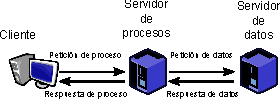
\includegraphics[width=0.75\textwidth]{Servidores_y_clientes_remotos/Datos_y_procesos_remotos.pdf}
\caption{\small Esquema de acceso a un servicio de procesos remotos, el cual a su vez utiliza datos de un segundo servidor. El encadenamiento de procesos permite ampliar notablemente la utilidad de estos.}
\label{Fig:Datos_y_procesos_remotos} 
\end{figure}

\end{itemize}

\subsection{Clientes}

\index{Cliente}
El cliente es el elemento que utiliza los datos proporcionados por el servicio. Para ello, realiza una petici�n a la que el servicio responde enviando dichos datos, que ser�n los que despu�s se emplear�n para realizar cualquier otra tarea, principalmente la representaci�n de estos para que el usuario pueda visualizarlos. El cliente es, de este modo, el intermediario entre el usuario y los servicios y datos que el servidor ofrece.

Como hemos visto al estudiar los servidores, las principales capacidades de estos implican la transmisi�n de im�genes con cartograf�a ya elaborada, o bien directamente capas, ya sean de tipo r�ster o vectoriales. En algunos casos, el servicio ofrecido es un servicio de procesos, pero su resultado generalmente es tambi�n una capa, por lo que, desde el punto de vista del cliente, la funcionalidad es en cierto modo similar (aunque internamente requiera una implementaci�n por completo distinta).

El cliente, por tanto, debe disponer de capacidades para formular peticiones a servidores como los anteriormente descritos, as� como para emplear las posibles respuestas que estos devolver�n. Estas �ltimas incluyen por lo general componentes de representaci�n, habitualmente con la forma t�pica de un visor en el que se permite cambiar la escala y desplazar la vista, tal y como ya vimos en el cap�tulo \ref{SIGs_escritorio}. No obstante, estas capacidades pueden variar ampliamente de un cliente a otro, desde el m�nimo necesario para simplemente representar los datos obtenidos del servidor hasta conjuntos de funcionalidades mucho m�s avanzadas pensadas para un uso intensivo de esos mismos datos.

Distinguimos as� dos tipos de clientes en funci�n de las capacidades que tengan: \emph{clientes ligeros} y \emph{clientes pesados}.

\begin{itemize}
	\item Cliente ligero. Se denomina \emph{ligero} por el tama�o relativamente reducido del programa en s�, lo cual va consecuentemente asociado a unas capacidades limitadas. Hablamos de clientes ligeros cuando nos referimos a \emph{Web Mapping} y a clientes que se ejecutan sobre un navegador Web, los cuales son siempre sencillos en cuanto a sus funcionalidades. En el momento de la carga de la p�gina Web que contiene al cliente, el navegador descarga toda la l�gica del programa, lo cual hace necesario limitar el tama�o de este.
	No obstante, los clientes Web empiezan progresivamente a ampliar sus posibilidades, y en ello juegan un importante papel otros servicios distintos a los de mapas o los de datos, como pueden ser los de procesos. Estos permiten que las funcionalidades adicionales no se implementen en el propio cliente (y por tanto sin aumentar en exceso su tama�o y sin disminuir su <<ligereza>>), sino que sean accedidas tambi�n como servicios remotos.
	La evoluci�n de la cartograf�a Web en esta direcci�n se dirige desde el \emph{Web Mapping} al \emph{Web GIS}, tal y como comentamos algunas p�ginas atr�s.
	\item Cliente pesado. A diferencia del cliente ligero, el cliente \emph{pesado} es una aplicaci�n individual que no se ejecuta sobre otra aplicaci�n soporte como puede ser un navegador Web. Al ser un programa independiente, debe ocuparse de toda la l�gica del proceso y de proveer todas las funcionalidades necesarias, por lo que su tama�o es generalmente mayor. Pese a ello, un cliente pesado no ha de ser necesariamente m�s potente y con m�s funcionalidades que uno ligero (aunque habitualmente lo es), ya que existen aplicaciones muy sencillas con capacidad para conectarse a servicios de mapas, que ofrecen poco m�s que un visor de cartograf�a. La diferencia no estriba en las capacidades del programa, sino en el enfoque a la hora de implementar este y el uso o no de otra aplicaci�n <<plataforma>>, generalmente en forma de un navegador Web.
	Los clientes pesados suelen permitir el uso de datos no procedentes directamente del acceso a servicios, tales como datos en ficheros locales, y no est�n pensados exclusivamente como clientes, sino como aplicaciones m�s amplias que adem�s disponen de capacidades para aprovechar un determinado tipo de servicios. Dicho de otro modo, un cliente pesado tal y como un SIG de escritorio tiene utilidad aunque no se emplee como cliente de ning�n servicio y no se disponga de conexi�n a red alguna, ya que puede alimentarse con datos locales y todas sus restantes funcionalidades (an�lisis, preparaci�n de cartograf�a, etc.) pueden aprovecharse con dichos datos.
\end{itemize}

\index{Cliente!ligero}\index{Cliente!pesado}

\section{Limitaciones y problemas de la cartograf�a Web}

Trasladar las ideas de los SIG de escritorio a la Web no es sencillo, por cuanto el entorno en el que nos movemos es muy distinto en uno y otro caso. La Web tiene sus propias limitaciones e inconvenientes, que en muchos casos no existen en el caso de una aplicaci�n de escritorio, y este hecho presenta dificultades complejas de salvar, obligando a desarrollar soluciones alternativas.

Una limitaci�n b�sica es la impuesta por el propio navegador como marco de trabajo. Las propias ventajas que este aporta son tambi�n responsables de ciertas limitaciones, ya que en el desarrollo de una aplicaci�n SIG Web no se tiene la misma libertad que al desarrollar una aplicaci�n de escritorio. Este no es un problema exclusivo del \emph{Web Mapping}, sino en general de todas las aplicaciones Web, que, pese a los avances que han tenido lugar en este sentido y la r�pido evoluci�n de las tecnolog�as Web, siguen sin poder ofrecer exactamente las mismas funcionalidades en lo que a interfaces respecta. 


A lo anterior debemos sumar el hecho de que las tecnolog�as Web en general son recientes y en cierto modo inmaduras, y aunque se emplea gran cantidad de medios y esfuerzo en el �mbito Web debido a su vital importancia en la actualidad, una buena parte de los elementos tecnol�gicos sobre los que se fundamenta el \emph{Web Mapping} actual no est�n todav�a completamente desarrollados y necesitan a�n evolucionar.

El aspecto m�s problem�tico es, no obstante, la propia red, especialmente en lo que respecta a su fiabilidad y rendimiento. Todos los datos que el cliente emplea en una aplicaci�n de cartograf�a Web provienen de la red, y por tanto existe una fuerte dependencia entre la aplicaci�n y el funcionamiento tanto de esta como del servidor que a trav�s de ella nos proporciona esos datos.

Si abrimos un archivo con datos espaciales en nuestro ordenador desde un SIG de escritorio, podemos casi garantizar que esa misma operaci�n funcionar� de igual modo si la repetimos en otro momento. Tener esa misma seguridad cuando se trabaja con datos remotos no es tan sencillo, ya que la red puede no funcionar o el servidor puede estar recibiendo en este momento gran cantidad de peticiones de otros clientes y no ser capaz de gestionarlas eficientemente y ofrecernos al instante respuesta a nuestra petici�n. En definitiva, las mismas circunstancias que afectan a todas las aplicaciones Web y que son conocidas por todos.

El rendimiento de la red es m�s importante a�n si cabe en el caso de trabajar con informaci�n geogr�fica, ya que los datos suelen ser voluminosos. Visualizar un mapa y que este pueda desplazarse y modificarse de forma igual de fluida que al trabajar con una aplicaci�n de escritorio requiere por un lado un ancho de banda suficiente para transmitir la gran cantidad de datos necesarios, y por otro la implementaci�n de algunas t�cnicas particulares que facilitan este proceso. Por su importancia, veremos en detalle las t�cnicas de \emph{tiling} (divisi�n horizontal de los datos geogr�ficos en teselas) y \emph{cacheo} (almacenamiento temporal de datos en la m�quina del cliente), utilizadas habitualmente en la actualidad.

\subsection{\emph{Tiling} y \emph{cacheo}}

\index{Tiling}\index{Cacheo}

Dos t�cnicas b�sicas que se emplean actualmente en los clientes Web que manejan informaci�n geogr�fica son el \emph{tiling} y el \emph{cacheo}. Estas t�cnicas permiten que la experiencia de trabajar con informaci�n geogr�fica dentro de una aplicaci�n SIG Web sea m�s agradable, logrando una mayor fluidez y superando en cierta medida las limitaciones de la red. Aunque es cierto que cada vez disfrutamos de mayores anchos de banda y velocidades de transmisi�n m�s altas, tambi�n aumentan de igual modo los vol�menes de datos manejados, con lo que las dificultades siguen existiendo de manera similar.

Ambas t�cnicas se utilizan en servicios en los que el servidor provee im�genes, ya que es en estos en los que resultan aplicables, y tambi�n donde es m�s necesario recurrir a este tipo de t�cnicas.

El \emph{tiling} es una t�cnica consistente en dividir las im�genes con las que se trabaja en im�genes menores que formen un mosaico. Esto permite un trabajo m�s r�pido, al utilizar unidades m�nimas de menor tama�o y poder reducir la necesidad de transmitir datos a trav�s de la red si se realiza una gesti�n correcta del conjunto de elementos de ese mosaico.

Esta divisi�n es similar en forma a la propia que se da en los datos originales, ya que, como sabemos (v�ase secci�n \ref{divisionHorizontal}), estos tambi�n se encuentran divididos horizontalmente. No obstante, se trata de una estrategia propia del sistema cliente--servidor, que divide las propias im�genes que luego se representar�n en este �ltimo, de forma que en lugar de transmitir una �nica imagen se transmiten varias de menor tama�o y la informaci�n correspondiente a la posici�n relativa de estas.

El \emph{cacheo}, por su parte, es una t�cnica no exclusiva del �mbito SIG, sino de la Web en general, y consiste en almacenar de forma temporal los datos obtenidos de un servidor en la m�quina local o bien en una m�quina intermedia (\emph{proxy}\index{Proxy}). De este modo, si volviera a resultar necesario acceder a esos datos, no han de pedirse al servidor, sino que pueden recuperarse de la copia local, con las ventajas que ello tiene en cuanto a la velocidad de acceso y la fiabilidad del proceso.

El uso conjunto de \emph{tiling} y \emph{cacheo} puede disminuir sensiblemente el volumen de datos a transmitir para, por ejemplo, modificar el encuadre de un mapa en una aplicaci�n SIG Web. La figura \ref{Fig:Tiling} muestra un ejemplo sencillo que servir� para comprender el ahorro de datos que puede conseguirse con el uso conjunto de estas t�cnicas.

\begin{figure}[!hbt]   
\centering
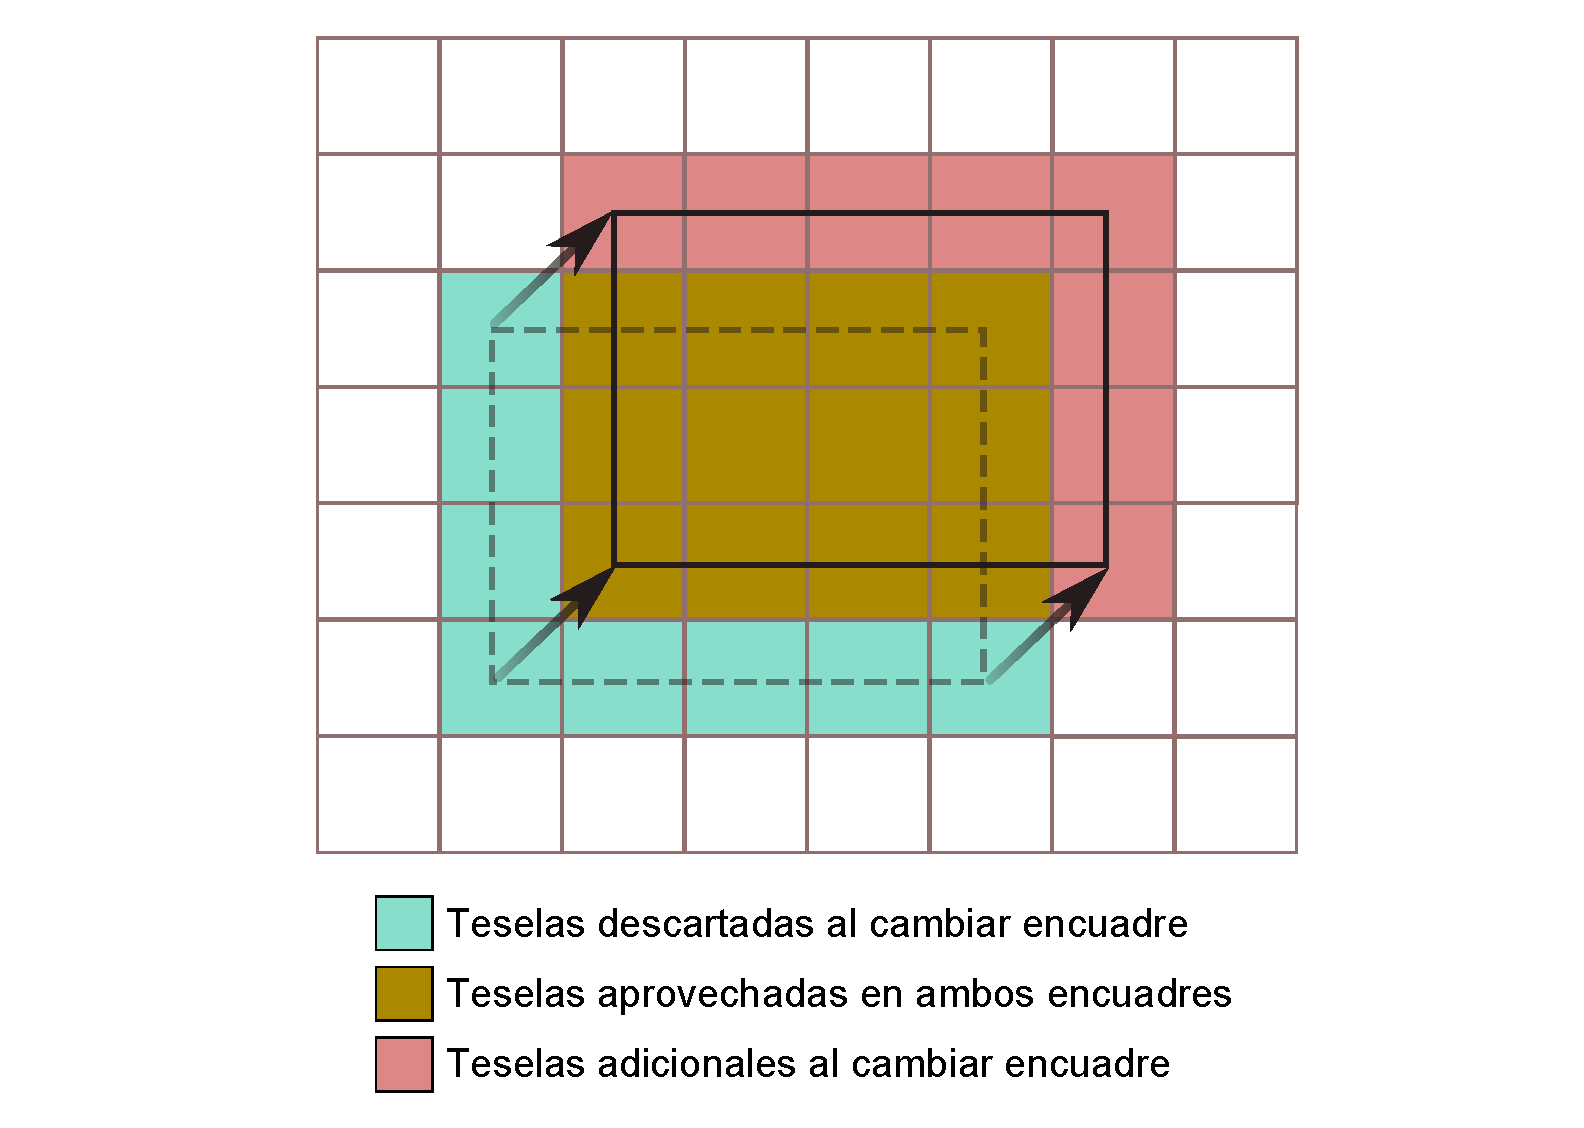
\includegraphics[width=.68\textwidth]{Servidores_y_clientes_remotos/Tiling.pdf}
\caption{\small Esquema del uso de \emph{tiling} y \emph{cacheo} para optimizar la transmisi�n de datos en una aplicaci�n SIG Web}
\label{Fig:Tiling} 
\end{figure}

En la figura puede verse del dato global al que se accede, dividido en una serie de unidades. Ello no quiere decir que el dato tenga ese n�mero de divisiones o que existan otros tantos ficheros. Puede tratarse de un �nico fichero, o de un n�mero muy elevado de ellos. Las divisiones se realizan a efectos de crear el mosaico de im�genes a la hora de transmitir estas.

Inicialmente, la aplicaci�n Web encuadra una regi�n que cubre 20 elementos o teselas. Si el usuario desplaza el encuadre para que cubra otro �rea distinta, como en el caso mostrado en la figura, el cliente realizar� una nueva petici�n y obtendr� una nueva imagen, que tendr� exactamente el tama�o con que esa imagen va a representarse. Este es exactamente el mismo tama�o que la imagen que encontramos inicialmente en el encuadre original, y por tanto la representaci�n de este encuadre original y posteriormente el encuadre modificado requiere transmitir dos im�genes que cubren cada una de ellas veinte teselas.

Si, por el contrario, aplicamos conjuntamente las t�cnicas anteriores de \emph{tiling} y \emph{cacheo}, al variar el encuadre no es necesario obtener del servidor una imagen que cubra todo el �rea a representar, sino tan solo los 8 elementos correspondientes a la zona no cubierta por la imagen inicial, ya que los restantes ya habr�n sido obtenidos con anterioridad y se encontrar�n almacenados (\emph{cacheados}) en nuestro ordenador. Es decir, el cliente crea la imagen a representar con 8 subimagenes pedidas al servidor y otras 12 ya descargadas previamente, reduciendo sensiblemente el volumen de datos pedidos al servidor.

Cuando este esquema de funcionamiento se combina con tecnolog�as como AJAX, citada anteriormente, y que a�ade a su vez mayor fluidez y una mejor respuesta de la aplicaci�n Web, el resultado es una aplicaci�n SIG altamente funcional y cuyo comportamiento se asemeja en cuanto a rendimiento al de un SIG de escritorio trabajando con datos locales.\index{AJAX}

Este tipo de t�cnicas no son exclusivas de los SIG en Internet, sino que tambi�n se aplican por igual al caso de SIG de escritorio cuando estos act�an como clientes y acceden a datos remotos. Particularmente, son de especial relevancia en el caso de los globos tridimensionales, en los cuales estas mismas t�cnicas se aplican no solo para las im�genes a visualizar, sino tambi�n para los datos de elevaci�n empleados para dar forma al relieve.

La combinaci�n de \emph{tiling} y \emph{cacheo} se lleva a cabo a m�ltiples escalas, de forma que se reduce el n�mero de operaciones a realizar y se obtiene un mayor rendimiento. Se emplean las denominadas \emph{pir�mides}, que ya vimos en el apartado \ref{Generalizacion_en_SIG} dedicado a la generalizaci�n cartogr�fica en un SIG. Estas pueden ser empleadas tambi�n en el lado del servidor, incluso cuando este sirve mapas creados a partir de cartograf�a vectorial. Para evitar tener que rasterizar los datos vectoriales cada vez que se realiza una petici�n (lo cual supondr�a un gran coste en t�rminos de proceso), se rasterizan de antemano a distintas escalas, de forma que cuando el cliente efect�a la petici�n ya se dispone de una imagen que servirle, sea cual sea la escala que pida.\index{Pir�mides}.

\section{Resumen}

Hemos visto en este cap�tulo las ideas fundamentales del binomio cliente--servidor, tanto en su definici�n m�s general referente a servicios Web de cualquier tipo, como en aquellos espec�ficos del �mbito SIG. En base a esto, existen distintas formas de llevar a la red tanto los propios datos geogr�ficos como las funcionalidades principales de los SIG de escritorio, y que pueden variar en cuanto a su complejidad, desde simples mapas est�ticos hasta aplicaciones Web complejas. Pese a las elevadas posibilidades que existen hoy en d�a en cuanto a tecnolog�as Web, es importante conocer tambi�n las limitaciones del entorno de trabajo, las cuales derivan tanto de la propia red como de otros aspectos, por ejemplo el hecho de que la aplicaci�n Web se ejecute dentro de un navegador. Estas limitaciones llevan al desarrollo de t�cnicas particulares para optimizar el funcionamiento de las aplicaciones SIG Web, entre las que se han de destacar el \emph{tiling} y el \emph{cacheo}.

Asimismo, conocemos ya las funcionalidades principales que debe presentar un servidor para responder a las peticiones de un cliente SIG, que son principalmente servir representaciones de los datos geogr�ficos, servir los datos en s� o consultas sobre estos, o bien servir procesos de an�lisis basados en dichos datos.


\chapter{SIG m�vil}\label{Otros_tecnologia}

\begin{keypoints}
�Qu� entendemos por SIG m�vil? $\bullet$ �Qu� elementos incorpora? $\bullet$ �En qu� se diferencia de un SIG de escritorio? $\bullet$ �Para qu� puede emplearse y qu� aporta en el trabajo de campo? $\bullet$ �Qu� es un Servicio Basado en Localizaci�n?
\end{keypoints}

\bigskip

\begin{intro}

Los SIG no han sido ajenos a la popularizaci�n de las tecnolog�as m�viles y la imparable expansi�n que sufren en la actualidad. M�s a�n, trat�ndose de un �rea relacionada con el manejo de informaci�n geogr�fica y el an�lisis del medio, el aprovechamiento de tecnolog�as que permiten llevar el SIG directamente a ese medio e <<interactuar>> directamente con la informaci�n geogr�fica ha abierto nuevos horizontes dentro del mundo de los SIG. 

En este cap�tulo veremos las caracter�sticas de una nueva forma de SIG basada en su uso sobre dispositivos m�viles, y trataremos las nuevas posibilidades que esto ofrece. Asimismo, y puesto que los SIG m�viles se apoyan en otra serie de tecnolog�as (especialmente de comunicaci�n y posicionamiento), desarrollaremos estas para definir el marco tecnol�gico en el que se encuadra esta rama particular del SIG.
\end{intro}

\section{Introducci�n}\label{SIG_Moviles}

A lo largo de la historia de los SIG, han ido surgiendo nuevas tecnolog�as como consecuencia de los cambios que se han producido en los dispositivos sobre los que las aplicaciones de manejo de informaci�n geogr�fica pueden ejecutarse. La aparici�n de nuevo \emph{hardware} es seguida de cerca por los desarrolladores de \emph{software}, que adaptan sus aplicaciones para aprovechar las nuevas caracter�sticas de esos dispositivos. Esto, adem�s de impulsar el avance de las aplicaciones SIG al permitirles mayor potencia de proceso o mayores capacidades, en ocasiones trae consigo la aparici�n de ramas completamente nuevas cuando la tecnolog�a de los dispositivos da un salto cualitativo de grandes proporciones.

En el veloz avance que el \emph{hardware} sufre constantemente, uno de los cambios m�s radicales de los �ltimos tiempos es la cada vez mayor potencia y disponibilidad de elementos port�tiles. Esto ha propiciado la aparici�n del denominado \emph{SIG m�vil}, as� como una serie de tecnolog�as y herramientas relacionadas que van dando forma a un sector muy distinto de lo que el SIG cl�sico representa, pero con una innegable vinculaci�n con este.

La implicaci�n que estas nuevas tecnolog�as han tenido en el �mbito del SIG va m�s all� de expandir sus posibilidades. Como vimos en el cap�tulo dedicado a la historia de los SIG, los primeros programa SIG se ejecutaban sobre grandes m�quinas cuya adquisici�n estaba muy lejos del alcance del p�blico especializado, como suced�a con toda la tecnolog�a inform�tica de aquel entonces. El salto a los ordenadores personales fue decisivo para iniciar una popularizaci�n de los SIG y contribuir a que se convirtieran en herramientas imprescindibles en una buena parte de sus �mbitos de aplicaci�n, entrando con fuerza en muchos sectores.

Con la aparici�n de los dispositivos m�viles y el crecimiento del mercado en torno a ellos, los SIG han dado un nuevo salto cualitativo. No solo han alcanzado un nuevo tipo de dispositivos con capacidades muy interesantes relacionadas con la informaci�n geogr�fica (destacando entre ellas la capacidad de conocer la posici�n del dispositivo), sino tambi�n a un nuevo p�blico y a nuevos grupos de inter�s. Si con el salto a los ordenadores personales los SIG se hicieron m�s asequibles en t�rminos econ�micos y de especializaci�n inform�tica, con la entrada de los dispositivos m�viles se han hecho asequibles en lo que a conocimientos espec�ficos del �mbito geogr�fico y cartogr�fico respecta. La informaci�n geogr�fica se abre paso en un mercado no especializado y, no solo su uso, sino tambi�n su creaci�n, pasan ambos a ser actividades no exclusivas de los profesionales de este campo. Es un paso m�s all� en la labor que desde sus or�genes los SIG vienen realizando, esto es, facilitar el uso de informaci�n geogr�fica y dar presencia a esta en todos los terrenos, haciendo ver la importancia que tiene en la pr�ctica totalidad de �mbitos.

Algunas de las tecnolog�as y utilidades que aparecen con los SIG m�viles distan mucho de la idea cl�sica de SIG, y constituyen de por s� un territorio nuevo que difiere notablemente de cuanto hemos visto hasta el momento. No obstante, la relevancia que estas tecnolog�as han adquirido y, sobre todo, la que van a adquirir en los pr�ximos a�os, las hace merecedoras de un cap�tulo propio en este libro y de ser consideradas como parte muy importante del panorama actual del SIG.	


%Tanto los elementos relacionados con los datos como los correspondientes al SIG m�vil ser�n la base para este cap�tulo que cerrar� la parte dedicada a la tecnolog�a.

\section{Qu� es el SIG m�vil}\label{SIG_Moviles}

Comencemos viendo qu� entendemos por SIG m�vil y de qu� formas puede presentarse. Para ello, analicemos como hemos hecho en otros apartados una situaci�n habitual en el entorno de trabajo de un SIG, en particular la relativa a la creaci�n de datos geogr�ficos. Seg�n vimos en el cap�tulo \ref{Fuentes_datos}, una de las formas de obtener datos con los que trabajar en un SIG es la toma de estos directamente en campo y su posterior incorporaci�n dentro del SIG. Esto requer�a habitualmente la digitalizaci�n de los datos tomados, ya que dicha toma se desarrollaba en la mayor parte de los casos mediante medios anal�gicos. 

Una importante mejora en este proceso se dar�a si la recogida de datos se efectuara empleando medios digitales, ya que el resultado ser�a mucho m�s cercano a lo que posteriormente va a necesitarse para el trabajo en gabinete. Adem�s de esta ventaja inmediata y del ahorro de tiempo que traer�a consigo, existen otras ventajas directas que los medios digitales aportar�an. Por ejemplo, si en lugar de un dispositivo de toma de datos contamos con dos de ellos, es relativamente sencillo (especialmente si los dispositivos pueden comunicarse entre s�) replicar los datos tomados, teni�ndose as� una copia de seguridad que evitar� en gran medida la p�rdida de los datos tomados por circunstancias diversas. El software instalado en el dispositivo puede a su vez contar con elementos que efect�en alg�n tipo de control de calidad, asegur�ndose de que no se introducen por descuido valores err�neos o de que no se deja sin rellenar ning�n campo de un estadillo.

No obstante, y a pesar de que esa recogida de datos se realiza con el fin de tratar estos posteriormente con ayuda de un SIG, el SIG como tal no participa en el proceso de toma de datos, sino tan solo en el trabajo de gabinete. Los dispositivos que se lleven al campo, sean del tipo que sean, simplemente recogen una serie de valores introducidos por el operario correspondiente, del mismo modo que este los anotar�a en una libreta o estadillo. Sin embargo, nada impide que podamos llevar al campo una aplicaci�n SIG (por ejemplo, un SIG de escritorio), y que sea en ese SIG, adaptado a esa particular tarea o no, donde tomemos los datos y en el que nos apoyemos para realizar todas las tareas adicionales que el trabajo de campo requiere.

Llevar el SIG al campo y sacarlo de su lugar fijo en el gabinete es lo que da lugar al denominado \emph{SIG m�vil}, cuyas particularidades, como veremos, van m�s all� del mero hecho de una localizaci�n de trabajo distinta. Cuando hablamos de SIG m�vil, no nos referimos �nicamente a un SIG habitual ejecut�ndose en una plataforma m�vil, sino tambi�n a una filosof�a distinta a la que existe en el uso de otros elementos tecnol�gicos del �mbito SIG que ya conocemos, en una localizaci�n fija. Es decir, llevar el SIG al campo no conlleva tan solo un cambio f�sico del entorno de trabajo, sino tambi�n una notable adaptaci�n en otros aspectos.

Hoy en d�a son muchos los dispositivos que podemos emplear para disponer de una herramienta m�vil con capacidad de proceso. Sin ir m�s lejos, un ordenador port�til con una conexi�n inal�mbrica a Internet (empleando telefon�a m�vil de tercera generaci�n) nos servir�a para replicar en campo el entorno de trabajo de un SIG de escritorio, poniendo a nuestra disposici�n todas las capacidades de este. Esta soluci�n, no obstante, es poco pr�ctica, ya que, si bien es cierto que podemos <<mover>> un ordenador port�til con relativa facilidad, no es un dispositivo pensado para moverse mientras se encuentra en funcionamiento, con lo que m�s bien tendr�amos un \emph{SIG port�til} en lugar de un \emph{SIG m�vil}. Hay otros tipos de \emph{hardware} mucho m�s adecuados para este cometido, como pueden ser los siguientes (Figura \ref{Fig:TiposDispositivosMoviles}):

\begin{itemize}
	\item Unidades GPS (a).
	\item Tablet PC	(b).
	\item PDA (c).	
	\item Tel�fonos m�viles (d).
\end{itemize}

\index{GPS}\index{PDA}\index{Tel�fono m�vil}\index{Tablet PC}

\begin{figure}[!hbtp]   
	\centering
	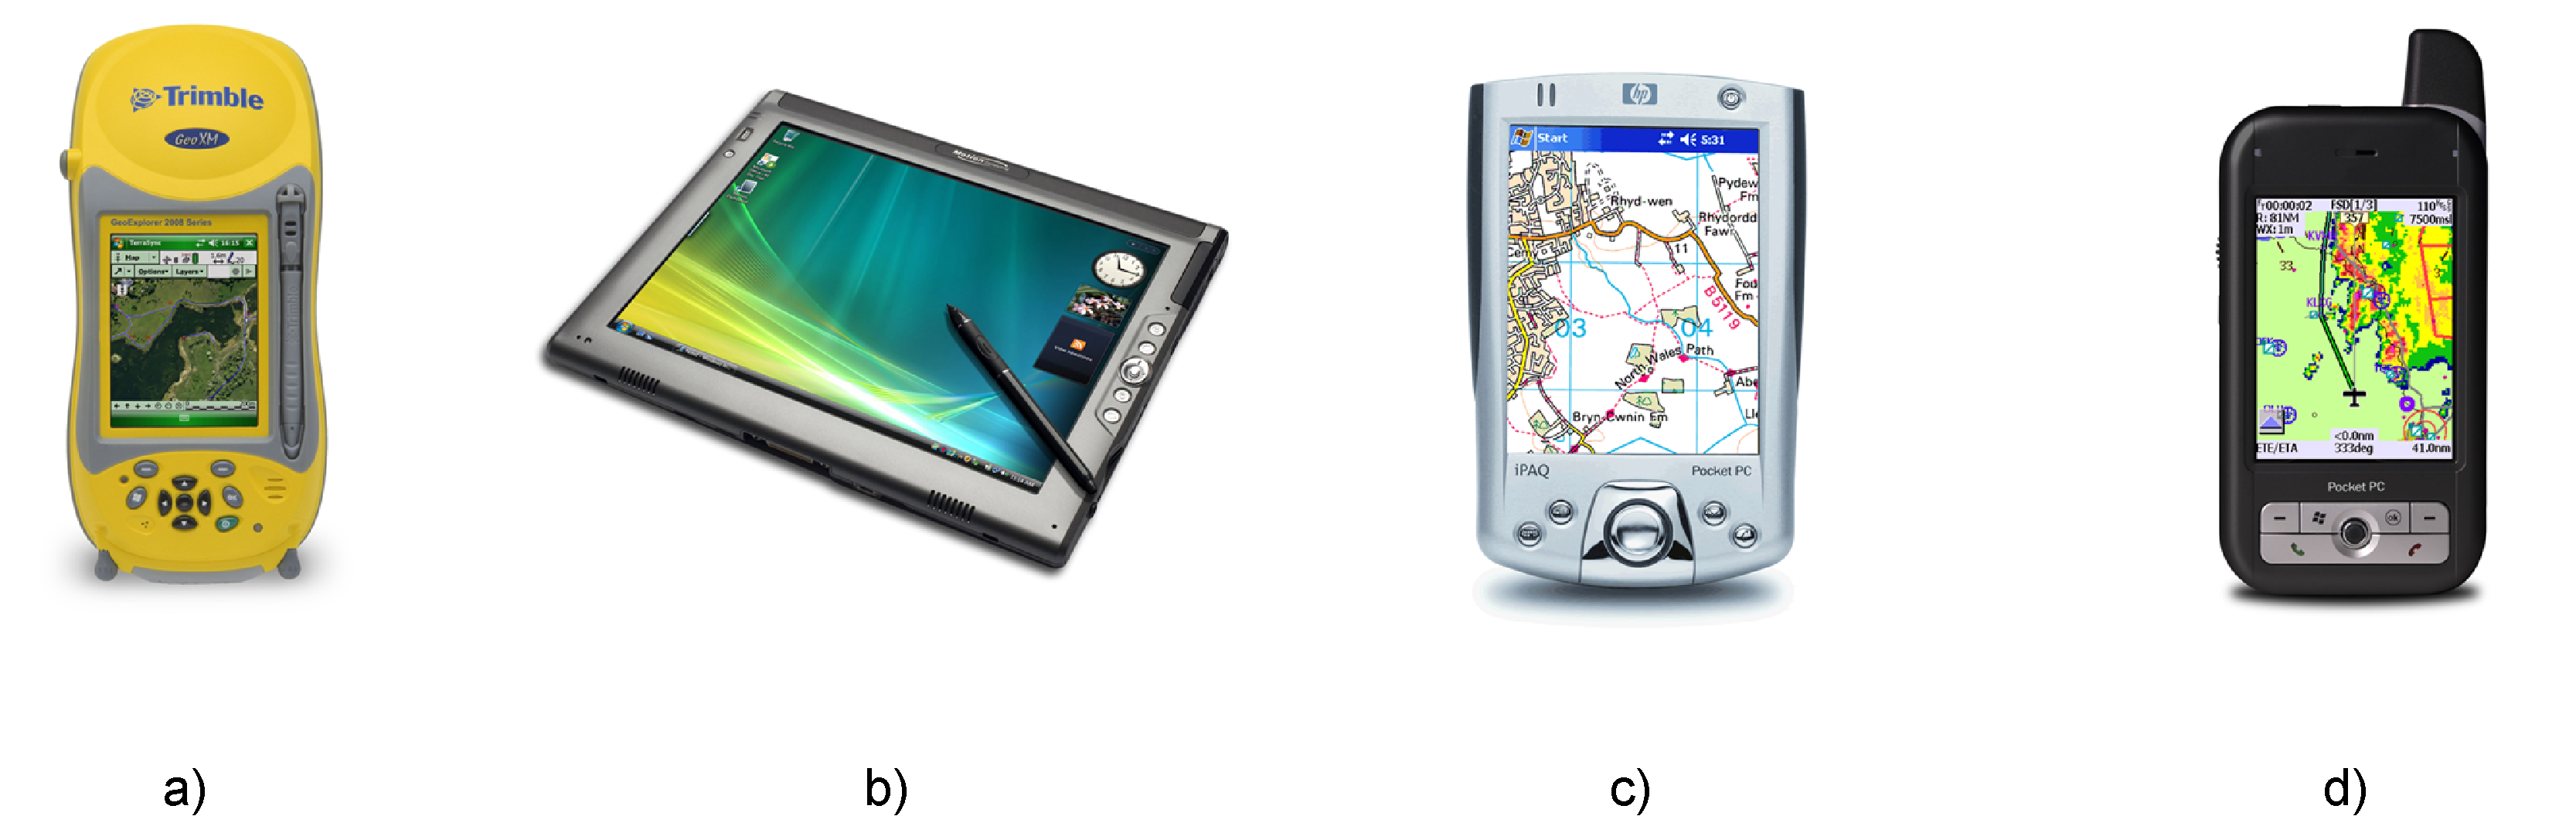
\includegraphics[width=0.90\textwidth]{Otros_tecnologia/TiposDispositivosMoviles.pdf}
	\caption{\small Distintos tipos de dispositivos m�viles}\label{Fig:TiposDispositivosMoviles} 
\end{figure}


Las caracter�sticas de estos dispositivos son distintas a las de un ordenador de sobremesa en el que utilizamos el \emph{software} SIG que hemos visto hasta ahora, haciendo que deba desarrollase software espec�fico y que deban tenerse en cuenta algunas consideraciones adicionales. A su vez, cada uno de los anteriores dispositivos tiene unas capacidades propias que lo hacen m�s interesante para unas u otras tareas dentro del trabajo en campo.

As�, las PDA y Tablet PC pueden considerarse como versiones reducidas de un ordenador de sobremesa o un ordenador port�til, y aunque en t�rminos de capacidad de almacenamiento y velocidad de proceso est�n por debajo de estos, son dispositivos de gran potencia que en muchos casos pueden ejecutar aplicaciones complejas o que requieran la realizaci�n de procesos intensos.

Por su parte, los tel�fonos m�viles son los dispositivos vers�tiles por excelencia y su penetraci�n es muy superior a la de cualquier otro.

Las unidades GPS m�s b�sicas se limitan a mostrar la localizaci�n, disponiendo de funcionalidades reducidas. Las m�s completas, no obstante, incorporan capacidades m�s cercanas a las de una PDA, con posibilidad de ejecutar aplicaciones complejas tales como un SIG adaptado. El inter�s de la tecnolog�a GPS est�, sin embargo, en considerarla como una tecnolog�a adicional que enriquece a algunos de los dispositivos anteriores. As�, tanto tel�fonos m�viles como PDA (o incluso otros dispositivos como c�maras fotogr�ficas) pueden incorporar receptores GPS y disponen por tanto de informaci�n acerca de su posici�n. Esta combinaci�n es la que da como resultado los dispositivos m�s potentes para el SIG m�vil, ofreciendo todas las funcionalidades que iremos viendo a lo largo de este apartado.

Asimismo, la conexi�n remota a Internet, que a d�a de hoy presenta un avanzado estado de desarrollo, abre la puerta a muchas de las capacidades m�s potentes y novedosas del SIG actual, como pueden ser la consulta o incluso la edici�n de cartograf�a, seg�n vimos en el cap�tulo \ref{Servidores_y_clientes_remotos}.

Para dar una definici�n m�s formal de lo que entendemos por SIG m�vil, podemos decir que es una tecnolog�a que integra una o m�s de las siguientes \cite{ESRI2007MobileGIS}:

\begin{itemize}
	\item Dispositivos m�viles.
	\item Sistemas de posicionamiento global (GPS).
	\item Acceso inal�mbrico a Internet.
\end{itemize}

Por su parte, \cite{Brimicombre2002GIS} distingue tres elementos principales que dan forma al contexto de las aplicaciones SIG m�viles: SIG, Internet, y dispositivos m�viles y Nuevas Tecnolog�as de la Informaci�n y la Comunicaci�n (NTIC). La figura \ref{Fig:LBSInterseccion} esquematiza esto.\index{NTIC}

\begin{figure}[!hbtp]   
	\centering
	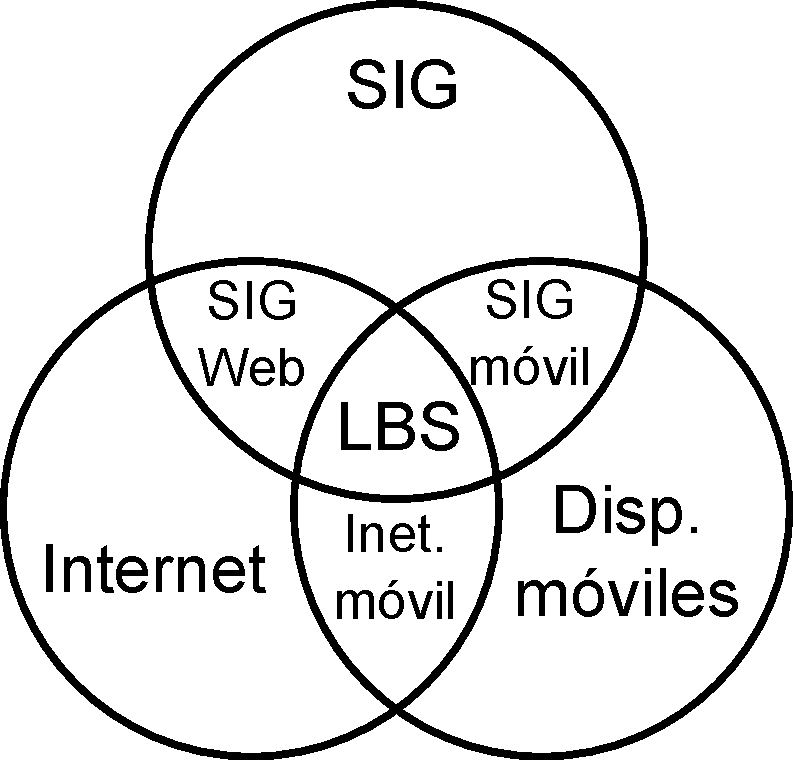
\includegraphics[width=0.35\mycolumnwidth]{Otros_tecnologia/LBSInterseccion.pdf}
	\caption{\small Clasificaci�n de aplicaciones del �mbito del SIG m�vil en funci�n de las tecnolog�as empleadas (seg�n \cite{Brimicombre2002GIS})}\label{Fig:LBSInterseccion} 
\end{figure}

En el centro, como tecnolog�as aglutinadoras de las anteriores, encontramos los \emph{Servicios Basados en Localizaci�n} (LBS\footnote{\emph{Location--Based Services}}). En general, se suelen recoger bajo esta denominaci�n los servicios que toman en consideraci�n la posici�n del usuario, y en los que se produce la participaci�n de un tercero, el encargado de proveer el servicio como parte fundamental de un negocio. Dichos servicios pueden ir desde la localizaci�n del comercio m�s pr�ximo hasta el env�o de avisos cuando se encuentre cerca de otro usuario conocido. 
\index{Servicios Basados en Localizaci�n}\index{Location--Based Services (LBS)|see{Servicios Basados en Localizaci�n}}

Podemos, con lo anterior, tener as� una primera y muy general clasificaci�n de las �reas de aplicaci�n del SIG m�vil en los dos siguientes grupos:

\begin{itemize}
	\item SIG <<en campo>>. Se centra m�s en los trabajos propios del SIG y en la recolecci�n y edici�n de datos.
	\item Servicios Basados en Localizaci�n. Servicios ofrecidos por terceros en funci�n de la posici�n del dispositivo y del usuario. 
\end{itemize}

En los LBS, la persona con el dispositivo es consumidor del servicio, mientras que en el SIG en campo su papel es principalmente como operario del SIG, y por tanto es esa persona la que provee un servicio o realiza una tarea apoyado en �l. Se tiende a concebir el LBS como un servicio no especializado cuyo consumidor no ha de estar necesariamente formado en las tecnolog�as SIG, mientras que en el caso del SIG en campo s� que debe tener unos conocimientos m�nimos, ya que su labor se desempe�a sobre una aplicaci�n SIG como tal. De los elementos que hemos comentado como integrantes del SIG m�vil, el LBS da mayor importancia al acceso a Internet y a la posici�n del dispositivo, dejando algo m�s de lado las capacidades cl�sicas del SIG. El SIG en campo, por su parte, hace �nfasis en esas capacidades, complement�ndolas con la movilidad del dispositivo y su capacidad para calcular su posici�n.

En nuestro supuesto con el que comenz�bamos esta secci�n, la toma de datos para ser posteriormente incorporados en un SIG, nos encontrar�amos en un claro caso de SIG en campo. Este tipo de enfoques surgieron antes que los LBS, ya que las tecnolog�as necesarias para estos �ltimos aparecieron con posterioridad. El SIG en campo no requiere obligatoriamente una conexi�n inal�mbrica, tecnolog�a de muy reciente aparici�n y, sobre todo, de muy reciente implantaci�n y desarrollo. La llegada de esta tecnolog�a, sin embargo, a�adi� nuevos elementos al SIG m�vil, y a d�a de hoy es la cabeza visible de este �mbito, especialmente por la gran expansi�n que ha supuesto para las tecnolog�as SIG. Como mencion�bamos en la introducci�n del cap�tulo, la popularizaci�n del SIG y sus elementos es el verdadero aspecto destacable del SIG m�vil.

Pese a lo anterior, la frontera entre estos dos grupos es difusa en cierto modo, ya que puede realizarse trabajo de campo aprovechando servicios de terceros a trav�s de Internet, y el usuario que aprovecha estos servicios (que pueden a su vez ser muy especializados) puede tener amplios conocimientos de SIG y realizar un trabajo altamente t�cnico. En relaci�n con cuanto hemos visto en otras partes del libro, el SIG en campo est�, a primera vista, m�s vinculado con todo ello, ya que el perfil de su usuario es m�s similar al del cl�sico usuario de SIG. La importancia que los LBS est�n teniendo es, no obstante, mucho mayor, ya que alcanza a todo el �mbito del SIG y tambi�n a grupos de usuarios muy alejados de ese perfil tradicional.

Independientemente de la naturaleza de la actividad realizada con un SIG m�vil, est� claro que este tiene unas particularidades que lo diferencian del SIG como hasta ahora lo hemos conocido, y que son las que, en gran medida, le confieren su potencia espec�fica como herramienta para trabajo sobre el terreno.

\section{Particularidades del SIG m�vil}

Los siguientes son algunos de los principales aspectos a considerar que caracterizan al SIG m�vil y lo diferencian del SIG cl�sico sobre una plataforma est�tica \cite{Solyman2005Directions}:

\begin{itemize}
	\item Variedad de plataformas. Mientras que en en caso de un SIG que se ejecuta en un ordenador de sobremesa las diferencias de plataforma son pr�cticamente inexistente (con, tal vez, la �nica salvedad del sistema operativo), en el caso del SIG m�vil la situaci�n es muy diferente. Existen plataformas muy diversas y dispositivos con caracter�sticas completamente distintas (por ejemplo, un tel�fono m�vil es, en ciertos aspectos, radicalmente distinto a un Tablet PC). Garantizar que todos estos dispositivos van a poder funcionar con una aplicaci�n requiere un esfuerzo extra a la hora de desarrollar esta.\index{Tablet PC}\index{Tel�fono m�vil}
	
	\item El usuario es parte de la informaci�n. El SIG nos permite analizar informaci�n muy variada, pero los an�lisis que realizamos se basan en unos datos concretos, ya sean estos locales o remotos. La posici�n de la maquina donde se ejecuta el SIG no es relevante ni tenida en cuenta, y ni siquiera existe la posibilidad de conocer y utilizar esta. En el SIG m�vil, por el contrario, la posici�n del dispositivo es conocida (si este integra alg�n tipo de mecanismo para calcular est�, de entre los que veremos m�s adelante en esta misma secci�n). Esa posici�n no solo puede ser empleada como otro dato m�s, sino que, en muchos casos, es el dato m�s importante y el que permite ofrecer servicios personalizados en funci�n de dicha posici�n. Indirectamente, el usuario se convierte tambi�n en parte de la informaci�n, ya que es \emph{su} posici�n la que ahora forma parte de esta.
	
	\item Acceso variable. La calidad del acceso a Internet va a fluctuar notablemente para un mismo conjunto de dispositivo, aplicaci�n, y usuario, ya que se trata de un servicio muy variable en funci�n de la localizaci�n. 
	
	\item Limitaci�n de los dispositivos. Comparados con un ordenador de sobremesa, que representa el dispositivo est�ndar en el que un SIG se ejecuta tradicionalmente, los dispositivos m�viles presentan importante limitaciones. Las m�s destacable de ellas es su propio tama�o, ya que las pantallas son peque�as y obligan a un uso distinto de su espacio para poder mostrar en ellas todos los elementos necesarios para garantizar una correcta usabilidad de las aplicaciones. Otras limitaciones son las ya mencionadas de almacenamiento y proceso. Y, por �ltimo, deben considerarse tambi�n las limitaciones en los dispositivos de entrada, muy distintos de los habituales teclado y rat�n, y sin apenas posibilidad de contar con otros perif�ricos m�s espec�ficos.\index{Usabilidad}
	
	\item Escalabilidad de los datos. Por las propias caracter�sticas tanto de los dispositivos como de sus conexiones, es necesario poner atenci�n en la escalabilidad de los datos para que las aplicaciones funcionen en circunstancias variadas, modificando el detalle en funci�n de las situaci�n.
\end{itemize}

\section{Aplicaciones del SIG m�vil}

Para estudiar las posibilidades que el SIG m�vil nos brinda, podemos analizar el papel que la informaci�n geogr�fica juega en el trabajo de campo. De este modo, descubriremos en qu� fases de este existir�n diferencias si podemos contar con una herramienta con las capacidades de un SIG, ampliada adem�s con otros elementos tales como un sistema GPS incorporado en el dispositivo. Entendemos aqu� trabajo de campo no en el sentido tradicional, sino como cualquier actividad desarrollada al aire libre en la que pueda aplicarse de alg�n modo un SIG m�vil, y que no necesariamente ha de constituir un <<trabajo>> como tal. 

Por una parte, la informaci�n geogr�fica es una herramienta en la que nos apoyamos para desarrollar la actividad en cuesti�n. Es decir, \emph{usamos} la informaci�n geogr�fica de forma directa. As� sucede, por ejemplo, cuando debemos tomar datos en una localizaci�n concreta como por ejemplo una parcela de inventario en un inventario forestal o un punto de alcantarillado para realizar un control del estado de una red de saneamiento. Tambi�n hacemos un uso similar cuando buscamos el restaurante m�s pr�ximo o queremos encontrar el camino m�s r�pido para tomar una carretera desde nuestro emplazamiento actual.

Tradicionalmente, la informaci�n geogr�fica se ha llevado al campo en forma de mapas impresos. Consultando estos se encontraba el lugar seleccionado y la forma de desplazarse hasta �l. Emple�bamos mapas topogr�ficos para encontrar esa parcela de inventario, callejeros para localizar la alcantarilla o un mapa de carreteras para saber c�mo desplazarnos en coche. Con el SIG m�vil, la informaci�n geogr�fica <<viaja>> al campo en formato digital, almacenada dentro del propio dispositivo o bien accediendo mediante este a informaci�n remota a trav�s de Internet. Esto ofrece ventajas tales como una mayor comodidad o como la posibilidad de tener varios dispositivos que compartan la cartograf�a. Es decir, varios t�cnicos que trabajen en campo pueden <<llevar>> el mismo mapa sin necesidad de tener varias copias de este, sino tan solo varias <<copias>> del dispositivo, que es por otra parte el mismo que emplear�n para la toma de datos o para cualquiera de las restantes tareas de su trabajo.

Por otra parte, la informaci�n geogr�fica en s� puede ser parte de la informaci�n recogida en campo. Es decir, es objeto de inter�s directo del trabajo de campo, y no solo un medio para realizar este. En este caso, los dispositivos m�viles van a permitir recoger con m�s precisi�n cualquier tipo de dato espacial sobre el terreno, al mismo tiempo que facilitan la creaci�n de dicho dato espacial o la edici�n de uno ya existente en funci�n de lo observado. Se unen en este punto la capacidad del dispositivo para conocer las coordenadas de su localizaci�n y las capacidades de las aplicaciones SIG para edici�n de datos, as� como las propias ventajas de los datos digitales en lo que a su actualizaci�n respecta (v�ase \ref{Datos_digitales_y_analogicos}). 

Esta es una de las razones principales del auge actual de los proyectos colaborativos para la creaci�n de cartograf�a (v�ase \ref{VGI}). Los complejos y caros equipos empleados en la cartograf�a cl�sica pueden sustituirse en muchos casos por dispositivos simples como un tel�fono m�vil o una unidad GPS de consumo, ambos sencillos de manejar para el usuario no especializado. Este puede as� tomar informaci�n geogr�fica y aportarla a alg�n proyecto comunitario, o bien guardarla para su uso personal. \index{VGI}

Con las ideas anteriores, podemos localizar las principales tareas que el SIG m�vil va a desarrollar en los distintos �mbitos de aplicaci�n y dividirlas en dos bloques: aquellas que permiten a los usuarios optimizar su movilidad durante el trabajo de campo, y aquellas que facilitan el desarrollo de la labor en cuesti�n una vez que se ha posicionado correctamente. 

Con respecto a las relacionadas con la movilidad, no se ha de pensar que estas se limitan a la localizaci�n de un emplazamiento puntual como se ha mencionado anteriormente, en lo que ser�a un uso casi exclusivo del sistema de posicionamiento del dispositivo. Tambi�n el an�lisis, parte importante de un SIG, puede servir para mejorar el desplazamiento que el trabajo en campo conlleva. El c�lculo de rutas es el principal ejemplo en este sentido, tal y como se implementa en los navegadores GPS, aunque no el �nico. Elaborar un plan de ruta en tiempo real puede ser �til para muchos profesionales, que pueden hacer uso de algoritmos como el del <<problema del viajante>> si estos se encuentran implementados en su SIG m�vil.

Dentro de las actividades que facilitan la labor en campo son de especial inter�s las relacionadas con la captura de informaci�n geogr�fica, que se simplifica notablemente como ya hemos dicho. Asimismo, tambi�n debemos citar cualquier tipo de servicio al que pueda accederse mediante la conexi�n inal�mbrica del dispositivo y proporcione informaci�n complementaria o alg�n tipo de apoyo a la persona que opera con este. Y por �ltimo, no ha de olvidarse el an�lisis SIG como una herramienta con gran utilidad, ya que permitir� realizar procesos adicionales que pueden a�adir nuevas posibilidades, tales como, por ejemplo, la validaci�n en tiempo real de los datos recogidos.

La siguiente lista resume algunas de las actividades principales que pueden llevarse a cabo con un SIG m�vil. Algunas de ellas pueden desarrollarse sin necesidad de contar con todos los elementos posibles (dispositivo, conexi�n inal�mbrica y sistema de posicionamiento), aunque buena parte requieren el concurso de todos ellos.

\begin{itemize}
	\item Navegaci�n. C�lculo de ruta �ptima entre dos puntos, guiado en interiores (centros comerciales, museos, etc.), aparcamiento guiado, gesti�n de
tr�fico. Una de las actividades m�s populares y extendidas.\index{Navegaci�n}
\item Inventario. Recogida de datos de cualquier tipo sobre el terreno. Cubre desde datos de inventarios forestales a prospecciones arqueol�gicas, pasando por datos censales o infraestructuras urbanas, entre muchos otros.
\item Informaci�n. Paginas amarillas espaciales o guias de viaje virtuales. En general, cualquier servicio de mapas o de puntos de inter�s con posici�n (monumentos, tiendas, aparcamientos...) accesible desde un dispositivo m�vil.
\item Emergencia. Localizaci�n de situaciones de emergencia, asistencia a veh�culos, optimizaci�n de asistencias y tiempos de respuesta. El usuario, ante una emergencia, puede conocer su posici�n e informar de ella, o bien a trav�s de la red puede conocerse esta y emplearse para dar una respuesta �ptima y una ayuda lo m�s eficiente posible.
\item Publicidad. Anuncios basados en localizaci�n, indicaci�n de negocios cercanos, promociones para comercios pr�ximos. Existen algunas limitaciones para evitar la publicidad no deseada, pero si el usuario da permiso, puede recibir informaci�n sobre posibilidades comerciales en su entorno.
\item Seguimiento. Tanto de personas como de productos, a lo largo de rutas predefinidas o no. Tambi�n puede servir para monitorizar una actividad en las distintas localizaciones por las que pase el usuario. Por ejemplo, una compa��a telef�nica puede estudiar los patrones de comportamiento en lo que al acceso a la red respecta, seg�n el emplazamiento desde el que se accede.
\item Gesti�n. Por ejemplo, de infraestructuras, de instalaciones, o de flotas. El dispositivo puede ir sobre el elemento a gestionar o bien emplearse para llegar hasta �l y efectuar all� alg�n tipo de control.
\item Ocio. Buscadores de amigos o juegos con componente espacial, entre otros.
\end{itemize}


\section{M�todos de posicionamiento}

\index{Metodos@M�todos!de posicionamiento}

Uno de los elementos clave del SIG m�vil es la capacidad de conocer la posici�n del dispositivo en todo momento, incorporando, como ya hemos visto, esa posici�n como un dato m�s de particular relevancia para realizar otras operaciones habituales del SIG o para ofrecer servicios de diversos tipos. Si el dispositivo en cuesti�n es una unidad GPS, est� claro que dispone de un sistema para obtener su posici�n, igual que sucede si se trata de otro tipo de dispositivo pero con un receptor GPS incorporado. Sin embargo, existen otras formas de que el dispositivo conozca su posici�n, y pueden emplearse de igual modo para obtener resultados similares en cuanto a las prestaciones que van a permitir.

Los m�todos mediante los cuales puede determinarse la posici�n de un dispositivo pueden clasificarse en tres tipos, a saber:

\begin{itemize}
	\item Introducci�n manual de la posici�n.
	\item M�todos basados en red.
	\item Metodos basados en terminal.
\end{itemize}

La introducci�n manual es el m�todo m�s obvio y simple que, no obstante, puede implicar tambi�n el uso de alg�n tipo de tecnolog�a y requiere algunas matizaciones. Adem�s de introducir directamente en el dispositivo las coordenadas actuales de este, es posible establecer una posici�n mediante la denominada \emph{geocodificaci�n inversa}. En el cap�tulo \ref{Geocodificacion} ve�amos que mediante la geocodificaci�n asign�bamos coordenadas a un determinado elemento, que pod�a ser un punto dado o cualquier otro elemento susceptible de ser georreferenciada. Aplicando este razonamiento de forma inversa, y si disponemos una base de datos con un conjunto de esos elementos y sus coordenadas asociadas, podemos obtener estas �ltimas haciendo b�squedas en esa base de datos con el nombre del elemento. Es decir, podemos decirle al dispositivo que la posici�n actual es \emph{Badajoz} o \emph{Estadio Vicente Calder�n} y �l se encargar� de convertir esa informaci�n en una coordenada num�rica similar a la que se obtendr�a si tuviera instalado un receptor GPS o alguna otra tecnolog�a similar.\index{GPS}\index{Geocodificaci�n}\index{Geocodificaci�n!inversa}

Algunos servicios de consulta de los que present�bamos en el cap�tulo \ref{Servidores_y_clientes_remotos} permiten este tipo de operaciones, y devuelven coordenadas asociadas a un determinado fen�meno geogr�fico. En particular, los denominadas servicios de \emph{Nomenclator} son los encargados de ello, como veremos con m�s detalle en el apartado \ref{Nomenclator}.\index{Nomenclator}

Con respecto a los dos tipos restantes, ambos se apoyan en una red de estaciones cuyas posiciones son conocidas. Los basados en red obtienen su posici�n mediante c�lculos realizados en funci�n de una se�al emitida por el dispositivo. El m�todo m�s habitual de esta clase es el empleado por los tel�fonos m�viles para calcular su posici�n en funci�n del repetidor m�s cercano de entre los que le ofrecen cobertura. 

Por el contrario, en los m�todos basados en terminal es el propio dispositivo el que recibe la se�al que procede de las estaciones, y en funci�n de estas calcula su posici�n. El sistema GPS es el ejemplo m�s popular de un m�todo de esta �ltima clase. Existen asimismo m�todos combinados que emplean ambas t�cnicas para el c�lculo posicional.

La figura \ref{Fig:MetodosPosicionamiento} esquematiza lo anterior.

\begin{figure}[!hbtp]   
	\centering
	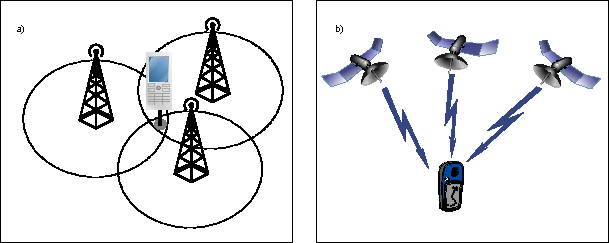
\includegraphics[width=0.95\textwidth]{Otros_tecnologia/MetodosPosicionamiento.pdf}
	\caption{\small Metodos de posicionamiento basados en red (a) y en terminal (b)}\label{Fig:MetodosPosicionamiento} 
\end{figure}

Con independencia del tipo de m�todo, el proceso de c�lculo de posici�n sigue un esquema como el siguiente:

\begin{itemize}
	\item La posici�n de las estaciones es conocida.
	\item La informaci�n de la se�al se transforma en una distancia (a excepci�n de si se aplica la t�cnica conocida como �ngulo de Llegada, que veremos seguidamente).
	\item La posici�n se calcula conociendo las distancias a un n�mero dado de estaciones base.
\end{itemize}

Esto coincide con lo que ya vimos en el apartado \ref{GPS} dedicado al sistema GPS.\index{GPS}

Para convertir la informaci�n de la se�al en una posici�n, encontramos diversas t�cnicas, a saber:

\begin{itemize}
	\item Celda de Origen (Cell of Origin, COO). Se identifica la estaci�n base m�s cercana y con ello se sabe que el dispositivo se encuentra en el per�metro de esta, dentro de su radio de alcance. La precisi�n depende de la densidad de la red. Para el caso de telefon�a m�vil, se sit�a entre los 200 metros y varios kil�metros, por lo que es baja para cierto tipo de servicios.
	\item Tiempo de Llegada (Time of Arrival, TOA). Se conoce la velocidad de transmisi�n de la se�al y el
tiempo entre el envio y la recepci�n de la se�al, con lo que puede calcularse la distancia. Se tiene as� la distancia respecto a una estaci�n dada. Considerando la velocidad de transmisi�n de la se�al, son necesarios relojes de alta precisi�n para lograr un calculo preciso.
\item Diferencia de Tiempo de Llegada (Time Difference of Arrival, TDOA) o Diferencia de Tiempo Observada Mejorada (Enhanced Observed Time Difference, E--OTD). En ambas t�cnicas se mide igualmente el tiempo, pero el c�lculo de la distancia se basa en la diferencia de las
se�ales de tres estaciones, pudi�ndose as� triangular la posici�n. En el caso de TDOA el c�lculo de la posici�n lo realiza el proveedor de la red, mientras que en el E--ODT es el dispositivo m�vil quien lo hace.
\item �ngulo de Llegada (Angle of arrival, AOA), Direcci�n de Llegada (DOA): Se usan antenas direccionables para detectar el �ngulo de llegada.
\end{itemize}\index{Angle of Arrival (AOA)}\index{Time Difference of Arrival (TDOA)}\index{Enhanced Observed Time Difference (E--OTD)}\index{Time Difference of Arrival (TDOA)}\index{Time of Arrival (TOA)}\index{Cell of Origin, (COO)}

Estas t�cnicas pueden emplearse simult�neamente, con objeto de proporcionar una localizaci�n m�s fiable o de adaptarse a las propias circunstancias de la red de estaciones en cada momento.

Es interesante mencionar que la precisi�n en los m�todos basados en terminal es en general mayor que la de los m�todos basados en red, siendo as� m�s adecuados para servicios en los que la posici�n deba conocerse de forma m�s precisa \cite{Lopez2004CRC}. As�, el GPS ofrece precisiones mucho mayores que las que se pueden obtener con la identificaci�n de la celda m�s cercana en una red de telefon�a m�vil. El GPS es, sin embargo, una t�cnica pensada para emplearse en exteriores, y los servicios en interior no pueden hacer uso de este, adem�s de requerir una precisi�n a�n mayor. En este caso, m�todos basados en redes locales inal�mbricas (WLAN), Bluetooth o ultrasonidos son una opci�n	v�lida, todos ellos tambi�n basados en terminal.\index{Bluetooth}\index{WLAN}

\section{Redes inal�mbricas}

Uno de los elementos m�s importantes en el SIG m�vil es la conexi�n inal�mbrica, que nos permite el acceso a Internet y poder acceder a todos los tipos de servicios a trav�s de esta. Sin conexi�n, disponemos de gran cantidad de funcionalidades, en especial aquellas fundamentales para lo que denomin�bamos SIG en campo. Podemos llevar el SIG m�vil y tomar datos, realizar an�lisis geogr�ficos sobre el terreno o navegar hasta una posici�n dada. Para ello solo necesitamos los datos que est�n almacenados en el propio dispositivo, tal y como sucede en un navegador GPS que contiene su propia cartograf�a.

Sin conexi�n a Internet, sin embargo, no se dispone de capacidad para recibir servicios ni tampoco para acceder a datos remotos o realizar consultas sobre datos de terceros, limitando as� de forma notable el alcance del  SIG m�vil. Siendo la conexi�n inal�mbrica un elemento tan relevante, es necesario conocer algunos fundamentos acerca de su funcionamiento y de c�mo los dispositivos habituales en el SIG m�vil incorporan la tecnolog�a correspondiente.

Existen dos esquemas principales para clasificar las redes inal�mbricas: seg�n la topolog�a de la red y seg�n su alcance

En relaci�n con la topolog�a de la red encontramos dos grupos: aquellas en que la red presenta una infraestructura formada por un n�mero de estaciones inm�viles (nodos) a las que acceden los terminales, y aquellas en las que los propios terminales forman una red \emph{ad--hoc}, siendo ellos mismos los nodos de esta.

Seg�n su alcance, y variando este de menor a mayor, podemos dividir las redes inal�mbricas en Redes Inal�mbricas de �rea Personal (Wireless Personal Area Network, WPAN), Redes Inal�mbricas de �rea Local (Wireless Local Area Network, WLAN) y Redes Inal�mbricas de �rea Amplia (Wireless  Wide Area Network, WWAN). Est� clasificaci�n se emplea con frecuencia, por lo que veremos los tipos anteriores con algo m�s de detalle.

Una red WPAN tiene un alcance corto, de unos 10 metros, y utiliza una frecuencia que no requiere de licencia para operar. La mayor�a de las redes de este tipo se basan en Bluetooth, y su velocidad de transmisi�n es de unos 0.5 Mbps.

Por su parte, una red WLAN tiene un alcance mayor, entre 10 y 100 metros, y su velocidad es muy superior, hasta los 100 Mbps. Utilizan tambi�n frecuencias sin necesidad de licencia. Las redes inal�mbricas de este tipo surgen a partir de las redes locales no inal�mbricas (LAN), principales pensadas para la transmisi�n de datos. Es por ello que esta tecnolog�a esta principalmente orientada a la transmisi�n de datos, y no ofrece soporte para voz como sucede con las redes WWAN.

Una red WWAN cubre un a distancia de entre 100 metros y 30 kil�metros, y emplea una frecuencia no libre, es decir, una cuyo uso requiere la adquisici�n de una licencia. Originalmente este tipo de redes se pensaron para transmisi�n de voz, por lo que su velocidad es baja, 4,8 kbps. La evoluci�n de estas redes para la transmisi�n de datos ha dado lugar a una segunda generaci�n con mayores velocidades, como sucede con las redes de los sistemas GSM (Global System for Mobile) o GRPS (General Packet Radio Service), con velocidades de 9,6--14 kbps y 20--115 kbps respectivamente. Estas velocidades siguen siendo insuficientes para gran cantidad de aplicaciones, pero las redes de tercera generaci�n, como el sistema UTMS (Universal Mobile Telecommunication System) europeo, pueden alcanzar tasas que permiten operar fluidamente del mismo modo que en una red local. 
\index{WWAN}\index{WPAN}\index{WWAN}\index{LAN}\index{General Packet Radio Service (GPRS)}\index{Global System for Mobile (GSM)}\index{Universal Mobile Telecommunication System}

\section{El \emph{sofware} SIG m�vil}

Conocemos ya los elementos que integran el SIG m�vil y las tecnolog�as implicadas tales como las redes inal�mbricas y los m�todos de posicionamiento. Es el momento de ver c�mo el \emph{software} SIG se adapta a estas circunstancias y cu�les son las caracter�sticas de las aplicaciones que vamos a encontrar sobre los dispositivos m�viles. 

Las diferencias entre los SIG de escritorio y los SIG sobre dispositivos m�viles vienen motivadas fundamentalmente por dos razones: las capacidades limitadas de estos (que mencionamos al inicio del cap�tulo) y las funcionalidades extras que presentan (principalmente la capacidad de posicionamiento). De igual modo, el enfoque y el tipo de uso que se pretenda dar condicionan la forma de las aplicaciones, existiendo una gran diferencia entre las aplicaciones dirigidas a lo que denomin�bamos SIG en campo y aquellas orientadas a los servicios basados en localizaci�n.

Comenzando con las primeras, representan el \emph{software} m�s similar a los SIG de escritorio, ya que las funcionalidades que resultan de inter�s son en buena medida aquellas que encontramos en estos. La lectura de datos y su representaci�n son de nuevo los pilares fundamentales entre las capacidades que una aplicaci�n para SIG en campo debe presentar, aunque tanto la edici�n como el an�lisis cobran relevancia y se implementan habitualmente para usos particulares. A su vez, tanto la lectura como la representaci�n de datos son dos de las �reas en las que es m�s necesaria una adaptaci�n debido a las limitaciones del dispositivo. 

En el caso de la lectura de datos, la limitada capacidad de almacenamiento y, sobre todo, memoria y velocidad de proceso, plantean un problema a la hora de desarrollar un \emph{software} que se comporte de manera similar a un SIG de escritorio. Aunque el desarrollo de ciertos tipos de dispositivos m�viles tales como las PDA es r�pido y sus capacidades casi alcanzan en algunos casos a las de un ordenador de sobremesa, el manejo de datos voluminosos sigue estando restringido. Este tipo de datos, no obstante, no son necesarios con tanta frecuencia como en el trabajo cl�sico con un SIG de sobremesa y, dado que otro tipo de funcionalidades est�n m�s limitadas, el rango de actividades que se van a desarrollar con tales datos es m�s reducido, lo que simplifica el desarrollo de todo lo relativo a su acceso y manejo.

Aunque un SIG m�vil era en su concepci�n inicial un elemento aut�nomo capaz de contener los datos necesarios para su funcionamiento e incluso incorporar nuevos datos mediante la creaci�n \emph{in situ} de estos, la aparici�n de las redes inal�mbricas ha cambiado esta tendencia y ahora el desarrollo se enfoca hacia el consumo de datos externos a trav�s de la red. Este planteamiento soluciona las dificultades que existen para la lectura de datos de gran volumen, ya que el dispositivo se convierte en un cliente y delega las tareas m�s costosas al servidor correspondiente. 

En los dispositivos de mayor potencia, adecuados para un desarrollo profesional del SIG en campo y para la recogida de datos, el SIG conserva sus capacidades de acceder a datos locales, mientras que en otros menos potentes y especializados, tales como tel�fonos m�viles, se consumen exclusivamente datos remotos. Algunas aplicaciones con base SIG, tales como navegadores, pueden utilizar cartograf�a digital almacenada en el dispositivo, pero la aplicaci�n como tal no permite la utilizaci�n de otros datos distintos o la lectura de diversos formatos, como s� sucede en un SIG de escritorio.

En lo referente a la representaci�n, la principal diferencia que se ha de considerar a la hora de dise�ar un SIG m�vil es, como parece l�gico, la reducida dimensi�n de las pantallas. Especialmente a la hora de visualizar datos y aplicar una simbolog�a a estos, se ha de tener en cuenta que existe una limitaci�n de tama�o y que no pueden aplicarse ideas id�nticas a las que ser�an adecuadas para una pantalla de ordenador com�n, ya que, al trasladarlas a la del dispositivo m�vil, puede obtenerse como resultado un mapa carente de utilidad que no transmite adecuadamente la informaci�n geogr�fica que contiene. Los conceptos de generalizaci�n cartogr�fica que mencionamos en el apartado \ref{GeneralizacionCartografica} (por ejemplo, la exageraci�n de elementos) han de tenerse muy presentes en la creaci�n de un SIG m�vil.

No solo en la forma de representaci�n existen diferencias, sino tambi�n en las propias funcionalidades de visualizaci�n incorporadas en la aplicaci�n. Esto est� relacionado no �nicamente con las limitaciones de la aplicaci�n ---podemos decir que, en general, el SIG sobre un dispositivo m�vil es una versi�n m�s simplificada y menos compleja de un SIG de escritorio---, sino con las necesidades que el usuario va a tener en este aspecto. 

Por ejemplo, podemos asumir que un usuario de un SIG m�vil va a requerir menos capacidades para establecer una representaci�n particular de los datos espaciales, ya que el trabajo que realiza es menos exigente en ese sentido. Mientras que sobre un SIG de escritorio se elabora cartograf�a y se trabaja con m�ltiples capas y en contextos de trabajo muy distintos, un usuario de un SIG m�vil emplea la representaci�n visual de los datos como forma de navegaci�n (de modo similar a como emplear�a un mapa en papel), o como un apoyo para la edici�n o toma de datos. En el primer caso, en la representaci�n debe primar la claridad, para facilitar la localizaci�n de aquello que busca. Aspectos relativos al an�lisis visual de la componente tem�tica del dato geogr�fico no son relevantes, ya que es raro que el usuario efect�e ese tipo de operaciones. En el segundo caso, debe prevalecer la representaci�n clara de aquello que se edita o de los elementos principales del entorno que van a servir de gu�a para la edici�n o creaci�n de nuevos datos.

Aunque tambi�n los SIG m�viles tienen parte del car�cter generalista de los SIG de escritorio, su contexto est� m�s acotado o, al menos, m�s limitado en cuanto a la extensi�n de las actividades que pueden llevarse a cabo y las necesidades que van a plantear. Por esta raz�n, sus funcionalidades, con la visualizaci�n en lugar predominante, tambi�n se encuentran limitadas.

Gracias al acceso a Internet que se mencion� anteriormente, no solo las tareas de acceso y procesado de datos se delegan en un servidor, sino tambi�n las relacionadas con la representaci�n. Por eso, es m�s habitual que los SIG m�viles act�en como clientes de servicios de mapas (es decir, de representaciones ya hechas y listas para visualizarse, como vimos en el apartado \ref{Servidores}), y no como clientes de servicios m�s complejos en los cuales se obtienen los datos y despu�s es la aplicaci�n la que se encarga de formar la representaci�n a partir de ellos. 

Esto no quiere decir que este tipo de capacidades no se encuentren en los SIG m�viles. De hecho, algunas aplicaciones SIG m�viles permiten incluso que la edici�n de la cartograf�a sea tambi�n un servicio remoto, es decir, que cuando el usuario edite o a�ada nuevos elementos en su trabajo de campo, estos cambios no tengan lugar en los datos locales que existen en el dispositivo, sino que modifica los presentes en un repositorio remoto. Esta funcionalidad, poco frecuente incluso en los SIG de escritorio m�s completos, aparece en algunos SIG m�viles. No obstante, las posibilidades de representaci�n son menores en el SIG m�vil, entendi�ndose que no es necesario ofrecer capacidades avanzadas de este tipo.

A modo de ejemplo, y tras lo explicado hasta este punto, se muestra en la figura \ref{Fig:SIGMovil} el aspecto de una aplicaci�n SIG m�vil.

\begin{figure}[!hbtp]   
	\centering
	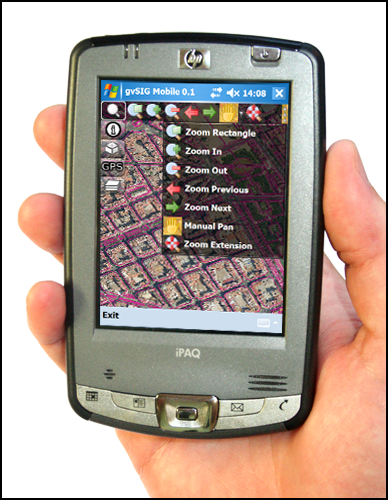
\includegraphics[width=0.4\textwidth]{Otros_tecnologia/SigMovil.png}
	\caption{\small Aspecto de una aplicaci�n SIG m�vil (gvSIG Mobile)}\label{Fig:SIGMovil} 
\end{figure}

En los servicios basados en localizaci�n, todo lo anterior tiene lugar de un modo a�n m�s patente, reduci�ndose por lo general m�s a�n las funcionalidades. El usuario tiene menos capacidad para <<operar>> con el dispositivo y con el \emph{software}, y los servicios se dise�an para que sean sencillos de consumir. Los tel�fonos m�viles, que representan el dispositivo por excelencia para este tipo de aplicaciones, tienen capacidades m�s reducidas que otros de los adecuados para el SIG m�vil, por lo que esta limitaci�n de funcionalidades es tambi�n producto del dispositivo al que est�n orientadas mayoritariamente. La menor especializaci�n de los usuarios influye tambi�n en que las aplicaciones presenten esas caracter�sticas.

La imagen \ref{Fig:EjemplosLBS} muestra dos ejemplos de aplicaciones para servicios basados en localizaci�n. Advi�rtase que estas no tienen necesariamente que guardar similitud con la idea cl�sica de un SIG, y que pueden no incluir ning�n tipo de representaci�n cartogr�fica. Es decir, que pueden proveer el servicio dando alg�n tipo de informaci�n geogr�fica (en el caso del ejemplo de la izquierda, se ofrecen mensajes de otros usuarios del servicio localizados en la misma zona) sin necesidad de mostrarla sobre un mapa. En el caso de la captura de pantalla mostrada en el lado derecho, la informaci�n s� aparece en un mapa, en el cual se muestran los contactos del usuario que se encuentran cercanos. El servicio en este caso es una forma particular de agenda de contactos que hace �nfasis en algunos de ellos en funci�n de su localizaci�n y la del usuario.

\begin{figure}[!hbtp]   
	\centering
	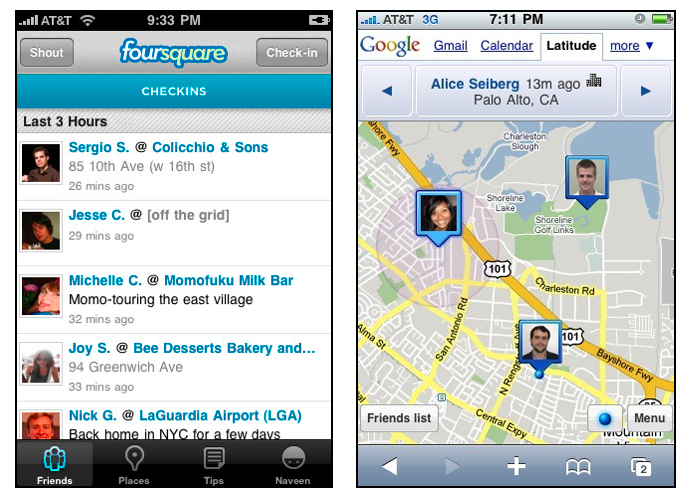
\includegraphics[width=0.7\textwidth]{Otros_tecnologia/EjemplosLBS.png}
	\caption{\small Dos servicios basados en localizacion sobre un tel�fono m�vil. A la izquierda, Foursquare[\url{http://www.foursquare.com}]. A la derecha, Google Latitude[\url{http://www.google.com/latitude}].}\label{Fig:EjemplosLBS} 
\end{figure}


\subsection{El contexto}

Un hecho b�sico a considerar a la hora de dise�ar \emph{software} para un SIG m�vil es que en este el \emph{software} conoce d�nde se encuentra el usuario, y el trabajo de dicho usuario normalmente se basa en emplear esa localizaci�n para realizar alg�n tipo de tarea. Aparece as� un concepto que carece pr�cticamente de importancia en un SIG de escritorio que se ejecuta sobre una m�quina inm�vil, pero que en el SIG m�vil y en cualquier otra aplicaci�n m�vil resulta fundamental: el \emph{contexto}.

\index{Contexto}

Entendemos por contexto toda aquella informaci�n que puede ser utilizada para caracterizar la situaci�n de una entidad. Una entidad es una persona, lugar o objeto que se considera relevante para la interacci�n entre el usuario y la aplicaci�n, pudiendo considerarse como entidad tambi�n a estos �ltimos \cite{Dey2001PUC}.

Los factores implicados en definir un contexto son variados, pero pueden considerarse divididos en cuatro grupos fundamentales \cite{Schilit1994IEEE}:

\begin{itemize}
	\item Contexto espacial. Caracterizado por d�nde se encuentra el usuario.
	\item Contexto social. Caracterizado por qui�n es el usuario.
	\item Contexto informacional. Caracterizado por qu� recursos se hallan cerca del usuario.
	\item Contexto t�cnico. Caracterizado por las caracter�sticas de la red y los dispositivos.
\end{itemize}

Si atendemos al caso particular de los servicios basados en mapas, \cite{Nivala2003HCI} propone los tipos de contexto que se detallan a continuaci�n:

\begin{itemize}
	\item Usuario. La identidad del usuario permite considerar aspectos tales como su edad y sexo (las cuales condicionan inevitablemente sus intereses), sus preferencias personales (por ejemplo, el idioma que habla y en el que quiere recibir el servicio) o quienes son su amistades y desea contactar con ellas.
	\item Localizaci�n. El elemento de contexto m�s empleado, puede ser tanto absoluta (expresada mediante una coordenada georeferenciada) o relativa a alg�n otro elemento que forma a su vez parte del contexto.
	\item Tiempo. Puede considerarse a distintas escalas. Por ejemplo, la hora del d�a (de inter�s si se busca un establecimiento para indicar al usuario solo aquellos que est�n abiertos en ese momento) o la estaci�n del a�o (que condiciona las actividades que se pueden realizar, ya que muchas de ellas son estacionales).
	\item Orientaci�n. Para saber hacia d�nde se dirige el usuario y conocer, por ejemplo, qu� tiene delante a la vista. Tambi�n para servicios de navegaci�n, para saber si el usuario sigue adecuadamente una ruta propuesta. Si el usuario se mueve, puede conocerse mediante el movimiento, pero en caso de estar parado requiere la presencia de elementos adicionales en el dispositivo.	
	\item Historial de navegaci�n. Permite crear un perfil del usuario y saber sus intereses en funci�n de los lugares en los que ha estado.
	\item Prop�sito de uso. Viene definido por las actividades y objetivos del usuario, as� como el papel que ejerce durante la utilizaci�n del dispositivo m�vil. Los distintos tipos de usuarios tendr�n diferentes necesidades en lo que respecta a la informaci�n, la presentaci�n (por ejemplo, mapas con una representaci�n m�s o menos t�cnica) o los modos de interacci�n con el dispositivo.
	\item Situaci�n cultural y social. La situaci�n de un usuario en este sentido se caracteriza por la proximidad a otros usuarios, su relaci�n social y sus tareas colaborativas.
	\item Entorno f�sico. En este apartado se incluyen elementos como la iluminaci�n existente o el ruido ambiente, que condicionan la interacci�n con el dispositivo y las capacidades del usuario de operar sobre �l.
	\item Propiedades del sistema. Se incluyen aqu� los aspectos relativos a la tecnolog�a. Por ejemplo, si el dispositivo es en color o en blanco y negro, si tiene teclado o pantalla t�ctil, o si la conexi�n a Internet es continua o intermitente.
\end{itemize}

Algunos de los anteriores puntos puede pensarse que no guardan una relaci�n directa con los LBS y no  han de ser exclusivos de estos. Es decir, que elementos como, por ejemplo, el tiempo, pueden ser tenidos en cuenta a la hora de proveer un servicio sin necesidad de que el dispositivo a trav�s del que se realiza dicho servicio cuente con medios para establecer su posici�n. Un ordenador de sobremesa, por ejemplo, tambi�n dispone de informaci�n sobre el tiempo que puede considerarse. Aunque esto es cierto, la inclusi�n del contexto espacial a�ade relevancia a los otros elementos del contexto, ya que modifica en gran medida la labor del usuario y la naturaleza de su actividad sobre el dispositivo.

Si recurrimos al cl�sico ejemplo del c�lculo de rutas, aunque el an�lisis llevado a cabo sea similar y requiera unos datos similares (punto de inicio, punto de destino y red de v�as de comunicaci�n), el hecho de que unos de dicho puntos (habitualmente el de salida) sea la coordenada actual del dispositivo modifica en gran medida muchos aspectos de esa operaci�n. Al realizar un c�lculo de rutas en un SIG de escritorio sobre un ordenador de sobremesa, lo normal es que este c�lculo nos sirva para planificar un viaje futuro o para estimar el tiempo que, en alg�n momento dado, tardaremos en cubrir la distancia entre dos puntos. 

Al contrario que en el caso de usar un dispositivo m�vil como un navegador GPS, ese viaje por esa ruta no vamos a realizarlo inmediatamente, no tiene necesariamente que ser un trayecto cercano a nuestra posici�n actual e incluso no vamos a ser nosotros mismos quienes hagamos el recorrido. De este modo, el contexto temporal o el personal del usuario no tienen significado alguno. Podemos incluir esas variables expl�citamente si el \emph{software} as� nos lo permite, pero no son una parte inherente al c�lculo y que siempre sea tenida en cuenta. Por su parte, en un dispositivo m�vil pueden incorporarse todos estos factores asumiendo que, en la mayor�a de los casos, s� van a ser de importancia. En resumen, que el hecho de que se trabaje sobre un dispositivo m�vil y este permita conocer su posici�n a�ade significado a todas las clases de contexto.

\begin{figure}[!hbtp]   
	\centering
	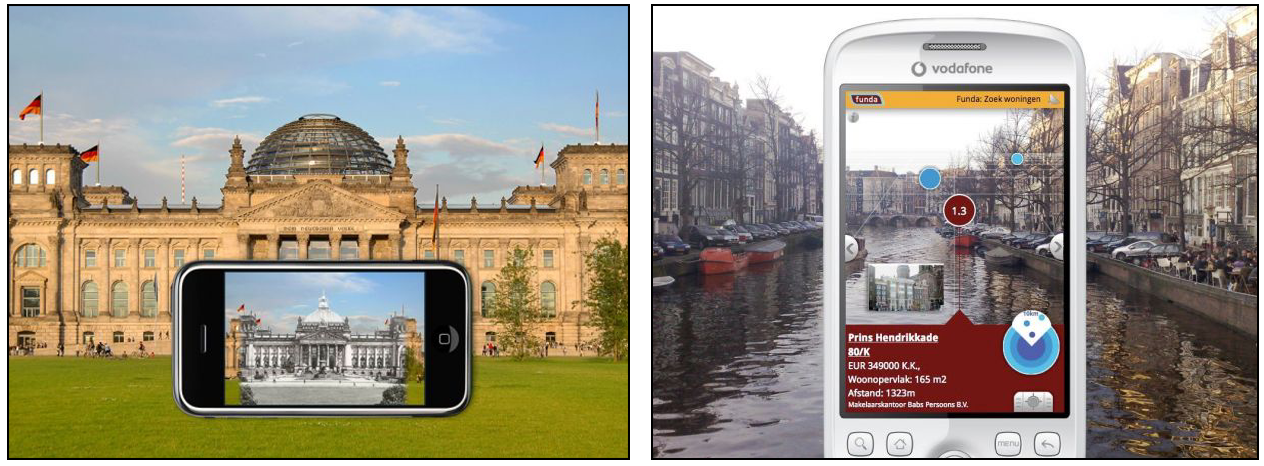
\includegraphics[width=\textwidth]{Otros_tecnologia/RealidadAumentada.png}
	\caption{\small Dos ejemplos de realidad aumentada (cortes�a de 5 Magazine)}\label{Fig:RealidadAumentada} 
\end{figure}

El \emph{software} debe dise�arse de forma que pueda responder a ese contexto y adaptarse a �l. Las siguientes son las �reas principales en las que esa adaptaci�n puede producirse \cite{Reichenbacher2004PhD}:

\begin{itemize}
	\item Informaci�n. La informaci�n proporcionada a un usuario var�a en funci�n del contexto en que se encuentre. Por ejemplo una b�squeda de un determinado tipo de comercio puede restringirse a un radio de alcance desde su posici�n habitual, o bien filtrarse para informar solo de aquellos que ofrezcan alg�n producto o servicio que sea de inter�s para el usuario.
\item Tecnolog�a. Conociendo las caracter�sticas del dispositivo, puede establecerse la mejor forma de ofrecer un servicio. Si, por ejemplo, la pantalla del dispositivo es demasiado reducida, no ser� interesante hacerlo mediante im�genes de gran tama�o, as� c�mo proveer alg�n tipo de informaci�n sonora si el dispositivo no dispone de capacidades para reproducir sonido. Como ya vimos, una de las caracter�sticas del SIG m�vil es la variedad de plataformas, por lo que la adaptaci�n en este sentido es importante para poder satisfacer las necesidades de los usuarios con independencia de qu� plataforma emplean.
\item Interfaz de usuario. El servicio puede alterar la interfaz sobre la que opera el usuario. El ejemplo m�s cl�sico es el desplazamiento de un mapa a medida que este se mueve.
\item Presentaci�n. Si la informaci�n requiere ser representada, esto puede hacerse de diversas formas en funci�n del contexto. La simbolog�a empleada se adapta, por ejemplo, a las preferencias del usuario (resaltando aquellos elementos que le resultan de mayor inter�s) o a la hora del d�a (se�alando de alg�n modo explicito el hecho de que algunos elementos pueden no estar disponibles, tales como comercios si es de madrugada), entre otros factores.
\end{itemize}

La adaptaci�n a un contexto dado puede ser mayor o menor en funci�n de las propias caracter�sticas del servicio y de c�mo este se plantee. En algunos casos puede llegar a ser muy intensa, tal y como sucede en la denominada \emph{realidad aumentada}, donde la frontera entre la realidad y el dispositivo se difumina gracias a que aquella se <<sumerge>> en este y es ampliada. En la realidad aumentada, vemos en la pantalla de nuestro dispositivo im�genes del entorno en el que nos encontramos, pero complementadas con elementos adicionales tales como gr�ficos, v�deos o sonido. Estos elementos es posible incorporarlos gracias a que se conoce con exactitud el contexto, y esa informaci�n puede emplearse para buscar nueva informaci�n que a�adir. La figura \ref{Fig:RealidadAumentada} muestra sendos ejemplos muy ilustrativos de lo anterior.\index{Realidad aumentada}
\section{Resumen}

Los SIG m�viles combinan las tecnolog�as SIG con los dispositivos m�viles, el acceso inal�mbrico a Internet y los sistemas de posicionamiento, para ofrecer una soluci�n ventajosa para el desarrollo de trabajo de campo. De particular inter�s son los denominados Servicios Basados en Localizaci�n, donde un tercero ofrece servicios que dependen de la posici�n en cada momento del dispositivo. Otras de las tareas fundamentales del SIG m�vil son la navegaci�n o la captura de datos espaciales directamente en el dispositivo, las cuales son las principales en lo que hemos denominado SIG <<en campo>>.

Para comprender el funcionamiento de las tecnolog�as implicadas en el SIG m�vil, hemos analizando por separado los m�todos de posicionamiento, las redes inal�mbricas y las aplicaciones de \emph{software}, cada una de las cuales desempe�a un papel b�sico en definir las capacidades de un sistema SIG m�vil.



